\section{Data}
\label{app:data}

\begin{table}[htbp]
\centering
\caption{Cohorts and datasets. Labels = binary labels (classification) or structures (segmentation); counts are cases in the training / selection / held-out splits as read from the manifests. Split rule: ``official val, halves'' = the official validation cases sorted by identifier and alternately assigned to the selection and held-out split; ``seeded'' = one fixed seeded division of the released labelled cases (80/10/10 of the released training data for the three RSNA and FDG cohorts, 70/15/15 for KiTS23 and MSD Pancreas, 91/20/20 volumes for LiTS); TotalSegmentator holds out its official test split and takes an equally large selection split from the official training split. FDG-PET/CT cases are studies (1014 studies of 900 patients; no patient spans splits); RSNA 2019 training cases are a stratified subset of the released training patients. Backbones: T = TAP-CT, S = SPECTRE, P = Pillar-0, V = VoCo.}
\label{tab:cohorts}
\adjustbox{max width=\textwidth}{\small
\begin{tabular}{@{}llllrrr@{}}
\toprule
Cohort / dataset & Labels & Split rule & Backbones & Train & Sel. & Held-out \\
\midrule
\multicolumn{7}{@{}l}{\textit{Classification}} \\
CVPR26: AMOS & 15 disease labels & official val, halves & T S & 1463$^\dagger$ & \numCasesCvprAmosVal & \numCasesCvprAmosTest \\
CVPR26: COVID-CTset & COVID-19 & official val, halves & T S & 308 & \numCasesCvprCovidVal & \numCasesCvprCovidTest \\
CVPR26: LUNA25 & nodule malignancy & official val, halves & T S & 1000 & \numCasesCvprLunaVal & \numCasesCvprLunaTest \\
FDG-PET/CT & 4 diagnosis groups & seeded, patient level & T S V & 776 & 116 & 122 \\
RSNA 2022 C-spine & patient, C1--C7 (8) & seeded, per study & T S V & 1615 & 202 & 202 \\
RSNA 2023 trauma & any, kidney, liver, spleen (4) & seeded, one series per patient & T S V & 2517 & 315 & 315 \\
RSNA 2019 hemorrhage & any + 5 subtypes (6) & stratified, patient level & T S P & 5000 & 3269 & 3264 \\
\addlinespace[2pt]
\multicolumn{7}{@{}l}{\textit{Segmentation}} \\
AMOS22 & 15 organs & official val, halves & T S V & 200 & 50 & 50 \\
KiTS23 & kidney, tumor, cyst & seeded & T S V & 343 & 73 & 73 \\
LiTS & liver, tumor & seeded & T S V & 91 & 20 & 20 \\
MSD Pancreas & pancreas, tumor & seeded & T S V & 197 & 42 & 42 \\
TotalSegmentator & 15 merged structures & official test held out & T S V & 1721 & 109 & 109 \\
\bottomrule
\end{tabular}}
\\[2pt]{\footnotesize $^\dagger$ distinct AMOS cases over the 15 per-label files; each label is known for a subset of cases.}
\end{table}

\begin{table}[htbp]
\centering
\caption{TotalSegmentator: the 117 released structures merged into 15 within anatomical systems, as implemented. Where two source masks overlap, the voxel is assigned to the smaller structure.}
\label{tab:totalseg}
\small
\begin{tabular}{@{}lp{0.72\textwidth}@{}}
\toprule
Structure & Source structures \\
\midrule
lungs and airway & five lung lobes, trachea \\
heart & heart, left atrial appendage \\
arteries & aorta, brachiocephalic trunk, left and right subclavian, common carotid and iliac arteries \\
veins & superior and inferior vena cava, left and right brachiocephalic and iliac veins, portal and splenic vein, pulmonary vein \\
liver & liver, gallbladder \\
spleen & spleen \\
pancreas & pancreas \\
kidneys & left and right kidney, left and right kidney cysts \\
GI tract & esophagus, stomach, duodenum, small bowel, colon \\
bladder and prostate & urinary bladder, prostate \\
glands & thyroid, left and right adrenal gland \\
brain and spinal cord & brain, spinal cord \\
spine & 25 vertebrae (C1--L6), sacrum \\
other bones & 24 ribs, sternum, costal cartilages, clavicles, scapulae, humeri, hip bones, femurs, skull \\
muscles & gluteus maximus, medius and minimus, iliopsoas, autochthon (left and right) \\
\bottomrule
\end{tabular}
\end{table}

\section{Training and evaluation details}
\label{app:details}

\begin{figure}[htbp]
\centering
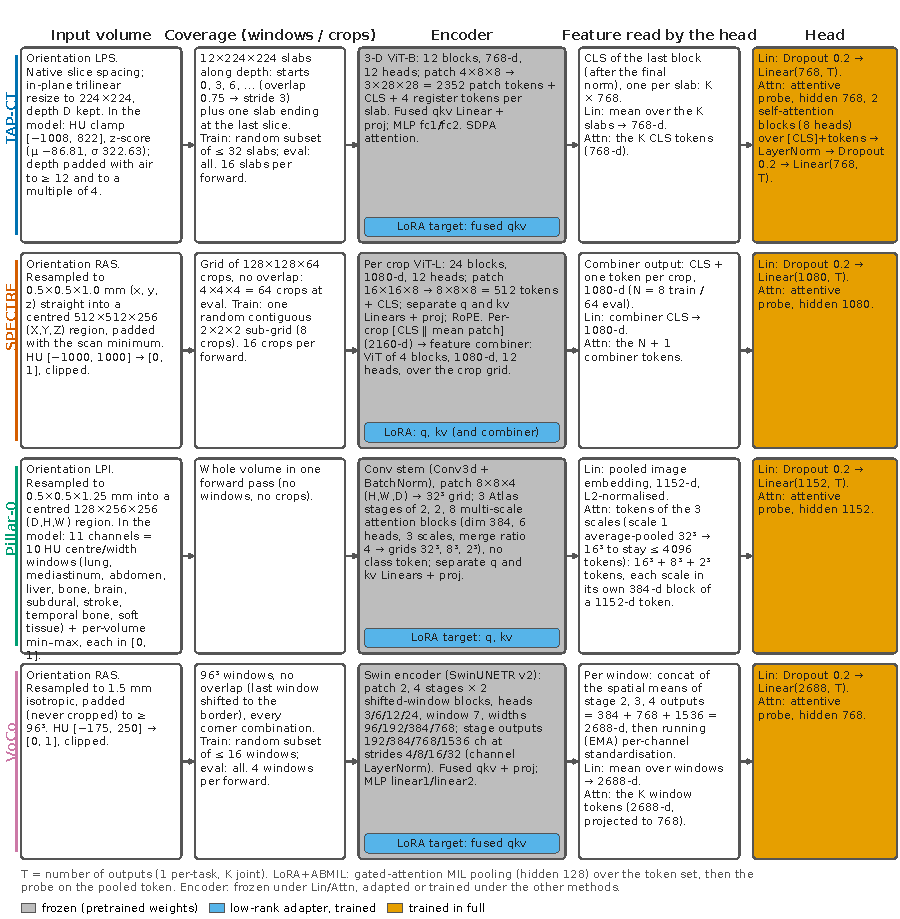
\includegraphics[width=\textwidth]{figures/fig_pipeline_cls.pdf}
\caption{Overview of the classification path, drawn from the implementation. Each row is one backbone: the volume is resampled and windowed as in pretraining, covered by windows or crops, encoded, and reduced to the feature the head reads. Lin reads one pooled feature per volume, Attn the set of window, crop or scale tokens. Grey = frozen, blue = low-rank adapter, orange = trained in full.}
\label{fig:pipeline_cls}
\end{figure}

\begin{figure}[htbp]
\centering
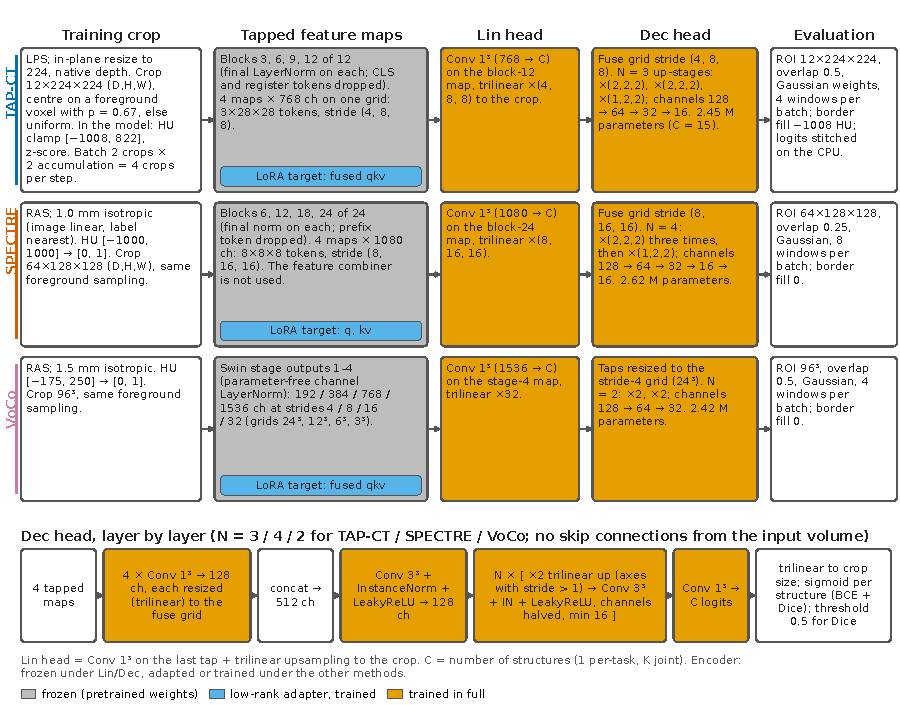
\includegraphics[width=\textwidth]{figures/fig_pipeline_seg.pdf}
\caption{Overview of the segmentation path, drawn from the implementation: crop geometry per backbone, the four tapped depths with their strides and channels, the linear probe on the deepest grid, and the multi-depth decoder layer by layer. Grey = frozen, blue = low-rank adapter, orange = trained in full.}
\label{fig:pipeline_seg}
\end{figure}

\begin{figure}[htbp]
\centering
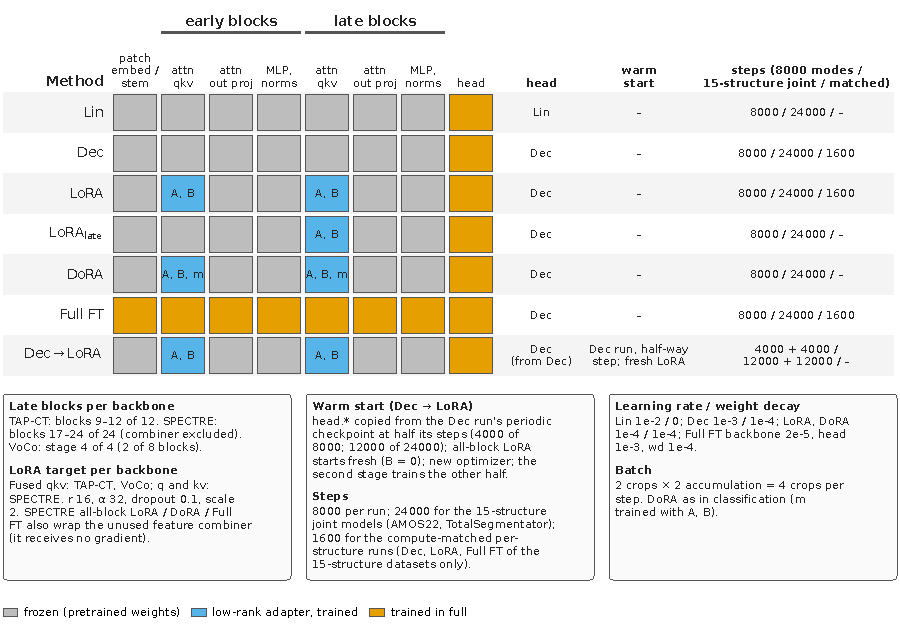
\includegraphics[width=\textwidth]{figures/fig_methods_seg.pdf}
\caption{What each segmentation method trains, the head it uses, its warm start and its budget.}
\label{fig:methods_seg}
\end{figure}

\begin{figure}[htbp]
\centering
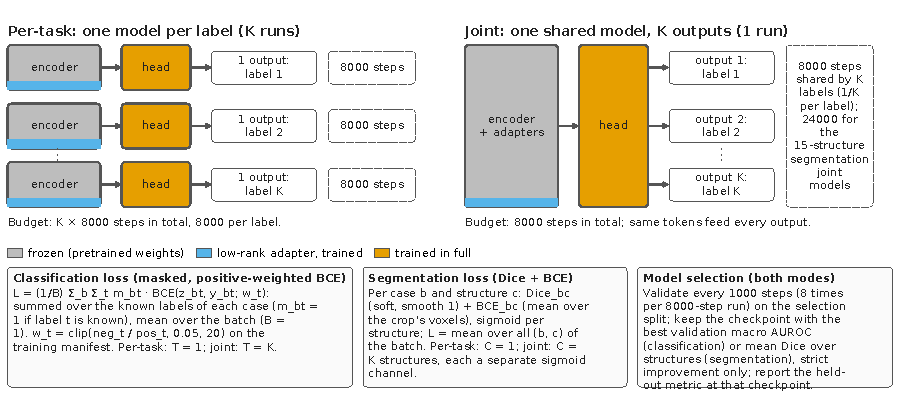
\includegraphics[width=\textwidth]{figures/fig_modes.pdf}
\caption{Per-task and joint training, the two losses, the step budgets and the selection rule.}
\label{fig:modes}
\end{figure}

\paragraph{Input preprocessing.} Every volume is reoriented to the frame of the backbone's pretraining and resampled to its grid. TAP-CT: LPS, native slice spacing, in-plane trilinear resize to $224\times224$, depth padded with air to at least 12 slices and to a multiple of 4; HU clipped to $[-1008, 822]$ and standardised with the model's mean and standard deviation; windows of 12 slices with a stride of 3 slices plus a final window ending at the last slice (at most 32 windows per training step, all windows at evaluation). SPECTRE: RAS, $0.5\times0.5\times1$\,mm, centred $512\times512\times256$ field of view padded with the scan minimum, HU in $[-1000, 1000]$ scaled to $[0,1]$; a $4\times4\times4$ grid of 64 crops of $128\times128\times64$ voxels at evaluation and a random contiguous $2\times2\times2$ sub-grid of 8 crops at training; each crop is summarised by its CLS token concatenated with its mean patch token before the feature combiner. Pillar-0: LPI, $0.5\times0.5\times1.25$\,mm, centred $128\times256\times256$ volume, eleven input channels (ten fixed centre/width windows and a per-volume min--max channel), one forward pass; the linear head reads the model's L2-normalised pooled embedding (three scales concatenated, 1152-d), the attentive head reads the tokens of the three scales, any scale with more than 4096 tokens being average-pooled on its grid. VoCo: RAS, 1.5\,mm isotropic, HU in $[-175, 250]$ scaled to $[0,1]$, padded to at least $96^3$ and covered by non-overlapping $96^3$ windows (the last window shifted to the border; at most 16 windows per training step); each window becomes one 2688-dimensional token, the concatenation of the spatial means of the stage-2, 3 and 4 outputs, standardised per channel with running statistics (momentum 0.01) that are stored with the checkpoint. For segmentation, TAP-CT keeps the classification grid (in-plane 224, native depth) and crops of $12\times224\times224$ voxels; SPECTRE resamples to 1\,mm and uses crops of $64\times128\times128$ voxels; VoCo resamples to 1.5\,mm and uses $96^3$ crops. A training crop is centred on a random foreground voxel of the run's structures with probability 0.67 and placed uniformly otherwise; volumes smaller than the crop are padded with the image minimum. At evaluation the whole volume is covered by a sliding window with Gaussian weighting (overlap 0.5 for TAP-CT and VoCo, 0.25 for SPECTRE) and Dice is computed on the backbone's working grid, without post-processing.

\paragraph{Heads.} The linear head is dropout (0.2) followed by one linear layer on the pooled feature: the mean of the window CLS tokens for TAP-CT (768-d), the feature combiner's CLS token for SPECTRE (1080-d), the pooled image embedding for Pillar-0 (1152-d) and the mean window token for VoCo (2688-d). The attentive probe prepends a learnable CLS token to the token set (the window CLS tokens for TAP-CT, the combiner tokens for SPECTRE, the multi-scale tokens for Pillar-0, the window tokens for VoCo; VoCo's tokens are first projected from 2688 to 768 dimensions), applies two pre-norm transformer blocks with eight-head self-attention and a GELU feed-forward layer of ratio 4, normalises the CLS output and maps it through dropout (0.2) and a linear layer. LoRA+ABMIL pools the window or crop tokens by gated attention \citep{ilse2018abmil}, $a_i=\mathrm{softmax}_i\big(\bm{w}^\top(\tanh(\bm{V}\bm{x}_i)\odot\sigma(\bm{U}\bm{x}_i))\big)$ with hidden size 128, and feeds the pooled token to the attentive probe. The segmentation linear probe is a $1\times1\times1$ convolution on the deepest grid (TAP-CT block 12, SPECTRE block 24, VoCo stage 4 at stride 32), upsampled trilinearly. The decoder projects each of the four grids to 128 channels with a $1\times1\times1$ convolution, resizes them to a common grid (the token grid for the two ViTs, the stride-4 grid for VoCo), concatenates them (512 channels), fuses them with a $3^3$ convolution, instance normalisation and leaky ReLU to 128 channels, then applies stages of trilinear $\times2$ upsampling followed by the same convolution block that halves the channels (to a minimum of 16) until the voxel grid is reached (three stages for TAP-CT, four for SPECTRE, two for VoCo), and ends with a $1\times1\times1$ convolution to one logit per structure. It has 2.45\,M (TAP-CT), 2.62\,M (SPECTRE) and 2.42\,M (VoCo) parameters plus $17C$ or $33C$ for $C$ structures, and no skip connections from the input.

\paragraph{Adapters.} LoRA \citep{hu2022lora} replaces a frozen projection $\bm{W}_0\bm{x}$ by $\bm{W}_0\bm{x}+\tfrac{\alpha}{r}\bm{B}\bm{A}\,\mathrm{drop}(\bm{x})$ with $r=16$, $\alpha=32$ and dropout 0.1; $\bm{A}$ is initialised Kaiming-uniform and $\bm{B}$ at zero, so training starts from the pretrained model. It is applied to the fused query/key/value projection of every TAP-CT and VoCo block and to the separate query and key/value projections of every SPECTRE block, of SPECTRE's feature combiner, and of every Pillar-0 block. Late adapters cover TAP-CT blocks 9--12, SPECTRE blocks 17--24 and its feature combiner, the third stage of Pillar-0 (8 of 12 blocks) and the fourth stage of VoCo (2 of 8 blocks). rsLoRA scales the update by $\alpha/\sqrt{r}$ instead of $\alpha/r$. DoRA \citep{liu2024dora} rescales each row of the adapted weight to a learned magnitude $\bm{m}$, $\bm{W}=\bm{m}\odot(\bm{W}_0+\tfrac{\alpha}{r}\bm{B}\bm{A})/\lVert\bm{W}_0+\tfrac{\alpha}{r}\bm{B}\bm{A}\rVert_{\text{row}}$, with $\bm{m}$ initialised to the row norms of $\bm{W}_0$; the magnitude is a two-dimensional parameter and receives weight decay like the adapter matrices. Attention-only fine-tuning unfreezes every parameter of the attention modules that LoRA would adapt (query, key, value and output projections with their biases, and for VoCo the relative position bias). In segmentation the SPECTRE adapters and full fine-tuning also cover the feature combiner, which the segmentation path does not evaluate; those parameters receive no gradient.

\paragraph{Two-stage methods.} Lin$\to$LoRA and Attn$\to$LoRA take the probe weights (for VoCo also the running standardisation statistics of the window tokens) from the parent run's checkpoint at step 4000 of its 8000-step schedule, add late-block LoRA with $\bm{B}=0$, and train 4000 further steps with a fresh optimiser and schedule. Dec$\to$LoRA takes the decoder from the Dec run at the midpoint of its schedule (step 4000; step 12\,000 for the 24\,000-step joint models) and trains all-block LoRA with the decoder for the second half.

\paragraph{Optimisation.} AdamW uses $\beta=(0.9, 0.999)$ and $\epsilon=10^{-8}$ (the framework defaults; no run overrides them). The learning rate rises linearly from 1\% of its peak over the first 10\% of the steps and then follows a cosine to $10^{-6}$. Weight decay is applied to parameters of dimension two or more, excluding biases and normalisation weights. Gradients are not clipped. Classification trains at batch size 1 without gradient accumulation; segmentation at a micro-batch of 2 crops with accumulation 2, so four crops per step. The classification loss for a case with logits $\bm{z}$, labels $\bm{y}$ and known-label mask $\bm{m}$ is
\begin{equation}
\mathcal{L}_{\text{cls}}=\frac{1}{B}\sum_{b=1}^{B}\sum_{t} m_{bt}\,\mathrm{BCE}(z_{bt}, y_{bt}; w_t), \qquad w_t=\mathrm{clip}\Big(\frac{n^{-}_t}{n^{+}_t}, 0.05, 20\Big),
\label{eq:lcls}
\end{equation}
where $\mathrm{BCE}(\cdot;w_t)$ is the binary cross-entropy with positive weight $w_t$ computed from the negative and positive counts of label $t$ in the training split. The segmentation loss per case $b$ and structure $c$, with $\bm{p}=\sigma(\bm{z})$ over the $V$ voxels of a crop and reference $\bm{y}$, is
\begin{equation}
\mathcal{L}_{\text{seg}}=\frac{1}{BC}\sum_{b,c}\Big[1-\frac{2\sum_v p_{bcv}y_{bcv}+1}{\sum_v p_{bcv}+\sum_v y_{bcv}+1}+\frac{1}{V}\sum_v \mathrm{BCE}(z_{bcv},y_{bcv})\Big].
\label{eq:lseg}
\end{equation}
In the joint CVPR26 models the three sources are sampled in the ratio 10:8:8 (AMOS, COVID-CTset, LUNA25); every other run cycles one shuffled training set.

\begin{table}[htbp]
\centering
\caption{Classification settings per method. LoRA-type adapters have rank 16, $\alpha=32$ and dropout 0.1. Learning rate and weight decay apply to every trained parameter unless a backbone/head pair is given. All runs: AdamW, 8000 steps (two-stage: 4000 + 4000), batch size 1, warm-up 10\%, cosine to $10^{-6}$, bf16, head dropout 0.2.}
\label{tab:optim}
\adjustbox{max width=\textwidth}{\small
\begin{tabular}{@{}llll@{}}
\toprule
Method & Trained in the encoder & Head & Learning rate / weight decay \\
\midrule
Lin & nothing & linear & $10^{-3}$ / 0 \\
Attn & nothing & attentive & $10^{-4}$ / 0.01 \\
LoRA & LoRA on q, k, v of every block & attentive & $10^{-4}$ / 0.01 \\
LoRA$_{\text{late}}$ & LoRA on q, k, v of the late blocks & attentive & $10^{-4}$ / 0.01 \\
LoRA+ABMIL & as LoRA & ABMIL then attentive & $10^{-4}$ / 0.01 \\
DoRA & DoRA on q, k, v of every block & attentive & $10^{-4}$ / 0.01 \\
rsLoRA & LoRA, scale $\alpha/\sqrt{r}$ & attentive & $10^{-4}$ / 0.01 \\
Lin$\to$LoRA & late LoRA from step 4000 of Lin & linear (inherited) & $10^{-4}$ / 0.01 \\
Attn$\to$LoRA & late LoRA from step 4000 of Attn & attentive (inherited) & $10^{-4}$ / 0.01 \\
Attn-only FT & all attention parameters & attentive & encoder $2\times10^{-5}$ / 0.05, head $10^{-4}$ / 0.01 \\
Full FT & every parameter & attentive & encoder $2\times10^{-5}$ / 0.05, head $10^{-4}$ / 0.01 \\
\midrule
\multicolumn{4}{@{}l}{\textit{Repeats and controls (Appendix~\ref{app:revision})}} \\
Full FT, lower LR & every parameter & attentive & encoder $5\times10^{-6}$ / 0.05, head $10^{-4}$ / 0.01 \\
Full FT, layer decay & every parameter, LR $\times0.75$ per block from the top & attentive & encoder $2\times10^{-5}$ / 0.05, head $10^{-4}$ / 0.01 \\
Full FT, accumulation & every parameter; accumulation 8, clipping 1.0, 1000 steps & attentive & as Full FT \\
MLP-only FT & both MLP layers of every block & attentive & encoder $2\times10^{-5}$ / 0.05, head $10^{-4}$ / 0.01 \\
rsLoRA, matched LR & LoRA, scale $\alpha/\sqrt{r}$ & attentive & $2.5\times10^{-5}$ / 0.01 \\
\bottomrule
\end{tabular}}
\end{table}

\begin{table}[htbp]
\centering
\caption{Segmentation settings per method. All runs: AdamW, 8000 steps (24\,000 for the AMOS22 and TotalSegmentator joint models; two-stage methods split the budget in halves), four crops per step, warm-up 10\%, cosine to $10^{-6}$, bf16. LoRA-type adapters as in Table~\ref{tab:optim}.}
\label{tab:optimseg}
\adjustbox{max width=\textwidth}{\small
\begin{tabular}{@{}llll@{}}
\toprule
Method & Trained in the encoder & Head & Learning rate / weight decay \\
\midrule
Lin & nothing & linear probe & $10^{-2}$ / 0 \\
Dec & nothing & decoder & $10^{-3}$ / $10^{-4}$ \\
LoRA & LoRA on q, k, v of every block & decoder & $10^{-4}$ / $10^{-4}$ \\
LoRA$_{\text{late}}$ & LoRA on q, k, v of the late blocks & decoder & $10^{-4}$ / $10^{-4}$ \\
DoRA & DoRA on q, k, v of every block & decoder & $10^{-4}$ / $10^{-4}$ \\
Full FT & every parameter & decoder & encoder $2\times10^{-5}$, head $10^{-3}$ / $10^{-4}$ \\
Dec$\to$LoRA & all-block LoRA from the midpoint of Dec & decoder (inherited) & $10^{-4}$ / $10^{-4}$ \\
\midrule
\multicolumn{4}{@{}l}{\textit{Controls (Appendix~\ref{app:revision})}} \\
From scratch & every parameter, encoder re-initialised & decoder & as Full FT \\
Compute-matched per-structure & Dec, LoRA, Full FT at 1600 steps per structure & decoder & as above \\
\bottomrule
\end{tabular}}
\end{table}

\paragraph{Model selection and per-case outputs.} Every 1000 steps the selection and held-out splits are evaluated and a checkpoint of the trained parameters is written; the checkpoint with the highest selection macro AUROC (mean over labels with both classes present) or mean Dice (mean over structures of the mean over cases in which the structure is present in the reference or the prediction) is kept, ties keeping the earlier checkpoint. For TotalSegmentator only the selection split is evaluated during training; the held-out split is evaluated afterwards with the selected checkpoint, and the recomputed selection Dice is required to match the recorded value within 0.005. Per case, the held-out probability of every known label (classification) and the Dice of every structure (segmentation) at the selected checkpoint are stored and are the input of every number in this paper. Dice thresholds the logits at 0; a structure enters a case's mean when the reference or the prediction contains it, so a false-positive structure scores 0 and an absent, unpredicted structure is skipped.

\section{Statistical procedure}
\label{app:stats}
Every number in this paper is computed by one script from the stored per-case predictions of the selected checkpoint of every run (\numRunsAllN{} runs; the classification files hold the held-out probability of every known label of every case, the segmentation files the Dice of every structure of every case).

\paragraph{Per-run metrics.} AUROC is the Mann--Whitney statistic with midranks (tied scores count one half); a label is skipped for a run when its selection or held-out split has fewer than two cases or a single class, which did not occur. Dice per structure is the mean over the held-out cases in which the structure is present in the reference or the prediction; an absent, unpredicted structure is skipped and a false-positive structure counts as 0. Cohort and dataset means (Tables~\ref{tab:cls} and~\ref{tab:seg}) are means over the labels or structures of complete cells. The recomputed selection-split macro metric was compared with the value logged during training for every run: all \numSelcheckClsRunsN{} classification runs agree to $10^{-7}$, and all but one of the \numSelcheckSegRunsN{} segmentation runs within $2\times10^{-3}$ (\numSegrecompRunsN{} segmentation runs had their per-case Dice re-inferred from the selected checkpoint after training; the one exception differs by $2.01\times10^{-3}$).

\paragraph{Did-not-train rule.} For each backbone and method, the median over label--mode pairs of the standard deviation of the held-out probabilities is computed; a median below \numSpreadMinValue{} flags a method that did not train. Only SPECTRE Full FT is flagged (\numSpreadSpectreFullft{}; every other method on TAP-CT, SPECTRE and Pillar-0 is at least \numSpreadOthermin{}). It stays in the per-cohort tables, the paired tests and the Full FT $-$ Lin estimate, and leaves the ranks and every average over methods. VoCo spreads are reported (Table~\ref{tab:spread}) but the rule is not applied to VoCo, whose methods have small spreads at held-out AUROCs well above chance.

\paragraph{Paired tests.} Per backbone, cohort, mode (per-task, joint) and label, every method is compared with the baselines Lin, LoRA, Attn and Full FT (classification; two-sided DeLong test of the AUROC difference on the same cases \citep{delong1988}) or Lin, Dec and LoRA (segmentation; paired case bootstrap of the mean Dice difference, 4000 resamples shared by every comparison of the same group, two-sided bootstrap $p$). Pairs require identical case sets; none had to be skipped. $p$-values are Benjamini--Hochberg adjusted \citep{benjamini1995fdr} within each family of comparisons (task, baseline, VoCo or not), and ``significant'' means an adjusted $p$ below 0.05; \numDelongTestsN{} DeLong tests and \numSegpairedTestsN{} bootstrap tests were made.

\paragraph{Label-level estimates.} The unit is one label (structure) on one backbone. For a comparison A $-$ B its value is the mean over the per-task and joint modes of the difference of the two methods' held-out metric (both modes must exist); for joint minus per-task it is the mean over the methods trained in both modes. The reported mean is over the labels of a backbone, or pooled over TAP-CT, SPECTRE and Pillar-0 (\numCiClsloralinAllLabelsN{} label--backbone units in classification, \numCiSegdeclinAllLabelsN{} in segmentation). Its 95\% interval is a percentile bootstrap with 4000 resamples that draws cohort--backbone clusters with replacement, then labels within each drawn cluster, and then replaces each drawn label's value by one of 1000 case-level resamples of that label (positives and negatives resampled separately in classification, with the same case indices for every term of the difference; all cases in segmentation). Besides the comparisons with the linear probe (Lin) and the frozen decoder (Dec), every method with the attentive head is compared with the frozen attentive probe (matched head), and LoRA $-$ Lin is also computed without FDG-PET/CT and the COVID-CTset label. Table~\ref{tab:cis} also gives the interval without the case stage. The number of cohort--backbone clusters with a positive mean is reported next to every estimate.

\paragraph{Ranks.} A slot is a label (structure) on one backbone in one mode with every method of the task present (minus methods that did not train); methods are ranked by held-out AUROC or Dice with ties sharing the average rank. Classification has \numRankSlotsN{} slots over the three main backbones and \numVocorankSlotsN{} on VoCo; segmentation \numSegrankSlotsN{} and \numVocosegrankSlotsN{} (TotalSegmentator per-structure slots lack three methods and are not ranked).

\paragraph{Seeds, controls and convergence.} Seed repeats are compared through cohort means per seed and the number of cohort--seed pairs in which one method is ahead of another; full fine-tuning variants through the selection-split AUROC, the number of cohorts whose run trained (median spread at least \numSpreadMinValue{}) and, for the variant with the highest selection AUROC, its label-level difference to Lin and LoRA; compute-matched models through the mean over structures of joint minus matched Dice. Convergence is the share of runs whose selected checkpoint is the last or one of the last two validations. All random draws use fixed seeds, so the script is deterministic.


\section{Repeats and controls}
\label{app:revision}

\begin{table}[htbp]
\centering
\caption{Seed repeats of the classification joint models: held-out AUROC (mean over the labels of a cohort) for seeds 42, 43 and 44 per backbone, cohort and method, with the standard deviation across seeds.}
\label{tab:seedscls}
\adjustbox{max width=\textwidth}{\footnotesize\setlength{\tabcolsep}{3.5pt}
\begin{tabular}{@{}llcccccccccccccccc@{}}
\toprule
Backbone & Cohort & \multicolumn{4}{c}{Lin} & \multicolumn{4}{c}{LoRA} & \multicolumn{4}{c}{Attn-only FT} & \multicolumn{4}{c}{Full FT} \\
\cmidrule(lr){3-6}\cmidrule(lr){7-10}\cmidrule(lr){11-14}\cmidrule(lr){15-18}
 & & 42 & 43 & 44 & SD & 42 & 43 & 44 & SD & 42 & 43 & 44 & SD & 42 & 43 & 44 & SD \\
\midrule
TAP-CT & CVPR26 & 0.707 & 0.700 & 0.708 & 0.004 & 0.733 & 0.723 & 0.701 & 0.016 & 0.739 & 0.732 & 0.750 & 0.009 & 0.744 & 0.699 & 0.691 & 0.029 \\
 & FDG-PET/CT & 0.858 & 0.859 & 0.864 & 0.003 & 0.866 & 0.855 & 0.870 & 0.008 & 0.870 & 0.867 & 0.888 & 0.012 & 0.608 & 0.809 & 0.567 & 0.130 \\
 & RSNA 2022 C-spine & 0.626 & 0.628 & 0.616 & 0.006 & 0.714 & 0.648 & 0.616 & 0.050 & 0.712 & 0.687 & 0.675 & 0.019 & 0.732 & 0.690 & 0.662 & 0.035 \\
 & RSNA 2023 trauma & 0.739 & 0.746 & 0.731 & 0.008 & 0.757 & 0.762 & 0.760 & 0.002 & 0.833 & 0.875 & 0.817 & 0.030 & 0.881 & 0.612 & 0.888 & 0.157 \\
 & RSNA 2019 hemorrhage & 0.871 & 0.870 & 0.874 & 0.002 & 0.906 & 0.889 & 0.894 & 0.009 & 0.915 & 0.882 & 0.914 & 0.019 & 0.854 & 0.742 & 0.910 & 0.086 \\
\addlinespace
SPECTRE & CVPR26 & 0.702 & 0.714 & 0.717 & 0.008 & 0.716 & 0.765 & 0.740 & 0.024 & 0.740 & 0.784 & 0.753 & 0.023 & 0.575$^{\dagger}$ & -- & -- & -- \\
 & FDG-PET/CT & 0.884 & 0.890 & 0.887 & 0.003 & 0.901 & 0.901 & 0.901 & 0.000 & 0.906 & 0.917 & 0.906 & 0.006 & 0.673$^{\dagger}$ & -- & -- & -- \\
 & RSNA 2022 C-spine & 0.629 & 0.606 & 0.541 & 0.046 & 0.706 & 0.687 & 0.694 & 0.009 & 0.718 & 0.707 & 0.623 & 0.052 & 0.554$^{\dagger}$ & -- & -- & -- \\
 & RSNA 2023 trauma & 0.789 & 0.797 & 0.790 & 0.004 & 0.846 & 0.847 & 0.844 & 0.001 & 0.803 & 0.839 & 0.860 & 0.028 & 0.654$^{\dagger}$ & -- & -- & -- \\
\addlinespace
Pillar-0 & RSNA 2019 hemorrhage & 0.888 & 0.888 & 0.888 & 0.000 & 0.912 & 0.917 & 0.920 & 0.004 & 0.912 & 0.923 & 0.927 & 0.007 & 0.878 & 0.896 & 0.907 & 0.015 \\
\bottomrule
\end{tabular}
}
\end{table}

\begin{table}[htbp]
\centering
\caption{Seed repeats of the segmentation joint models: held-out Dice (mean over structures) for seeds 42, 43 and 44 per backbone, dataset and method, with the standard deviation across seeds.}
\label{tab:seedsseg}
\adjustbox{max width=\textwidth}{\footnotesize\setlength{\tabcolsep}{3.5pt}
\begin{tabular}{@{}llcccccccccccc@{}}
\toprule
Backbone & Dataset & \multicolumn{4}{c}{Dec} & \multicolumn{4}{c}{LoRA} & \multicolumn{4}{c}{Full FT} \\
\cmidrule(lr){3-6}\cmidrule(lr){7-10}\cmidrule(lr){11-14}
 & & 42 & 43 & 44 & SD & 42 & 43 & 44 & SD & 42 & 43 & 44 & SD \\
\midrule
TAP-CT & AMOS22 & 0.708 & 0.661 & 0.655 & 0.029 & 0.739 & 0.747 & 0.642 & 0.059 & 0.681 & 0.681 & 0.679 & 0.001 \\
 & KiTS23 & 0.514 & 0.519 & 0.515 & 0.003 & 0.582 & 0.573 & 0.572 & 0.005 & 0.519 & 0.524 & 0.545 & 0.014 \\
 & LiTS & 0.699 & 0.716 & 0.730 & 0.016 & 0.715 & 0.717 & 0.724 & 0.004 & 0.715 & 0.724 & 0.711 & 0.007 \\
 & MSD Pancreas & 0.480 & 0.478 & 0.483 & 0.002 & 0.505 & 0.495 & 0.487 & 0.009 & 0.487 & 0.480 & 0.437 & 0.027 \\
 & TotalSegmentator & 0.798 & 0.752 & 0.798 & 0.026 & 0.776 & 0.765 & 0.780 & 0.008 & 0.815 & 0.814 & 0.815 & 0.000 \\
\addlinespace
SPECTRE & AMOS22 & 0.658 & 0.658 & 0.659 & 0.000 & 0.784 & 0.762 & 0.779 & 0.011 & 0.669 & 0.666 & 0.672 & 0.003 \\
 & KiTS23 & 0.572 & 0.591 & 0.576 & 0.010 & 0.588 & 0.628 & 0.631 & 0.024 & 0.519 & 0.546 & 0.521 & 0.015 \\
 & LiTS & 0.742 & 0.741 & 0.740 & 0.001 & 0.753 & 0.729 & 0.736 & 0.012 & 0.713 & 0.722 & 0.685 & 0.019 \\
 & MSD Pancreas & 0.514 & 0.519 & 0.521 & 0.004 & 0.550 & 0.559 & 0.544 & 0.008 & 0.530 & 0.513 & 0.508 & 0.011 \\
 & TotalSegmentator & 0.770 & 0.726 & 0.728 & 0.025 & 0.733 & 0.750 & 0.773 & 0.020 & 0.795 & 0.747 & 0.745 & 0.028 \\
\bottomrule
\end{tabular}
}
\end{table}

\begin{figure}[htbp]
\centering
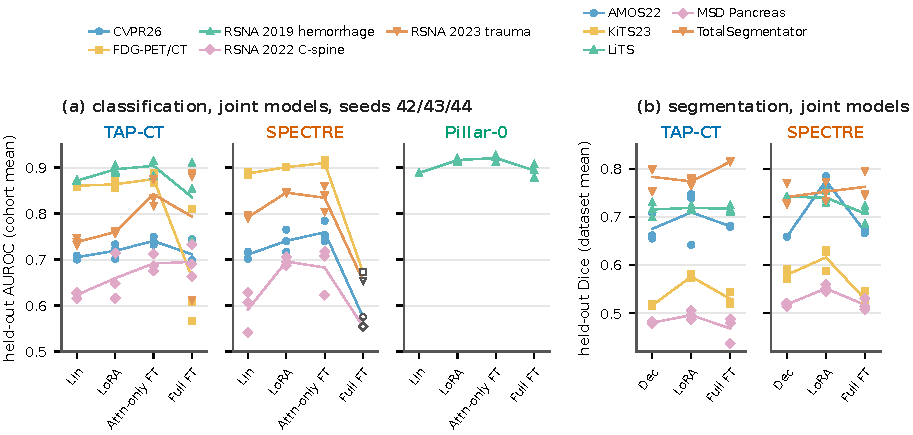
\includegraphics[width=\textwidth]{figures/fig_seeds.pdf}
\caption{Between-seed variation of the joint models next to between-method differences: cohort (dataset) means of the three seeds per method, (a) classification, (b) segmentation.}
\label{fig:seeds}
\end{figure}

\begin{table}[htbp]
\centering
\caption{Full fine-tuning settings and controls on the classification joint models: held-out AUROC per backbone and cohort for full fine-tuning with the default setting, a lower learning rate ($5\times10^{-6}$), layer-wise learning-rate decay (0.75 per block) and gradient accumulation with clipping, for MLP-only fine-tuning and for rsLoRA at a quarter of the learning rate, next to Lin and LoRA.}
\label{tab:revisioncls}
\adjustbox{max width=\textwidth}{\footnotesize\setlength{\tabcolsep}{3.5pt}
\begin{tabular}{@{}llccccccccc@{}}
\toprule
Backbone & Cohort (labels) & Lin & LoRA & \begin{tabular}[b]{@{}c@{}}Full\\FT\end{tabular} & \begin{tabular}[b]{@{}c@{}}Full FT,\\lower LR\end{tabular} & \begin{tabular}[b]{@{}c@{}}Full FT,\\layer decay\end{tabular} & \begin{tabular}[b]{@{}c@{}}Full FT,\\accumulation\end{tabular} & \begin{tabular}[b]{@{}c@{}}MLP-only\\FT\end{tabular} & rsLoRA & \begin{tabular}[b]{@{}c@{}}rsLoRA,\\matched LR\end{tabular} \\
\midrule
TAP-CT & CVPR26 (17) & 0.707 & 0.733 & 0.744 & 0.730 & \textbf{0.750} & 0.685 & \underline{0.745} & 0.722 & 0.741 \\
 & FDG-PET/CT (4) & 0.858 & \underline{0.866} & 0.608 & 0.861 & \textbf{0.867} & \textbf{0.867} & \underline{0.866} & 0.785 & 0.855 \\
 & RSNA 2022 C-spine (8) & 0.626 & \underline{0.714} & \textbf{0.732} & 0.654 & 0.618 & 0.687 & 0.627 & 0.601 & 0.611 \\
 & RSNA 2023 trauma (4) & 0.739 & 0.757 & \underline{0.881} & 0.860 & 0.869 & 0.758 & \textbf{0.894} & 0.684 & 0.751 \\
 & RSNA 2019 hemorrhage (6) & 0.871 & 0.906 & 0.854 & 0.889 & \textbf{0.917} & \underline{0.909} & 0.907 & 0.869 & 0.901 \\
\addlinespace
SPECTRE & CVPR26 (17) & 0.702 & 0.716 & 0.575$^{\dagger}$ & 0.713 & \textbf{0.758} & 0.511 & 0.681 & 0.690 & \underline{0.739} \\
 & FDG-PET/CT (4) & 0.884 & \underline{0.901} & 0.673$^{\dagger}$ & 0.884 & 0.865 & 0.883 & 0.814 & 0.900 & \textbf{0.908} \\
 & RSNA 2022 C-spine (8) & 0.629 & \textbf{0.706} & 0.554$^{\dagger}$ & 0.568 & \underline{0.700} & 0.553 & 0.626 & 0.691 & 0.672 \\
 & RSNA 2023 trauma (4) & 0.789 & 0.846 & 0.654$^{\dagger}$ & 0.793 & \textbf{0.863} & 0.578 & 0.838 & \underline{0.850} & 0.834 \\
\addlinespace
Pillar-0 & RSNA 2019 hemorrhage (6) & 0.888 & 0.912 & 0.878 & \textbf{0.924} & \underline{0.920} & 0.918 & 0.912 & 0.918 & \underline{0.920} \\
\bottomrule
\end{tabular}
}
\end{table}

\begin{table}[htbp]
\centering
\caption{Compute-matched segmentation: dataset-mean held-out Dice of the 24\,000-step joint model, of per-structure models trained for 1600 steps each (the same total number of steps) and their difference, for Dec, LoRA and Full FT on AMOS22 and TotalSegmentator.}
\label{tab:computematched}
\adjustbox{max width=\textwidth}{\footnotesize\begin{tabular}{@{}lllcccc@{}}
\toprule
Dataset (structures) & Backbone & Method & \begin{tabular}[b]{@{}c@{}}Joint\\{\scriptsize 24\,000 steps}\end{tabular} & \begin{tabular}[b]{@{}c@{}}Per-task, matched\\{\scriptsize 1600 steps each}\end{tabular} & Joint $-$ matched & \begin{tabular}[b]{@{}c@{}}Per-task\\{\scriptsize 8000 steps each}\end{tabular} \\
\midrule
AMOS22 (15) & TAP-CT & Dec & 0.708 & 0.763 & -0.055 & 0.793 \\
 &  & LoRA & 0.739 & 0.617 & +0.122 & 0.767 \\
 &  & Full FT & 0.681 & 0.766 & -0.085 & 0.805 \\
\addlinespace[2pt]
 & SPECTRE & Dec & 0.658 & 0.760 & -0.101 & 0.808 \\
 &  & LoRA & 0.784 & 0.648 & +0.136 & 0.812 \\
 &  & Full FT & 0.669 & 0.793 & -0.123 & 0.792 \\
\addlinespace
TotalSegmentator (15) & TAP-CT & Dec & 0.798 & 0.783 & +0.015 & 0.843 \\
 &  & LoRA & 0.776 & 0.657 & +0.119 & 0.819 \\
 &  & Full FT & 0.815 & 0.803 & +0.012 & 0.832 \\
\addlinespace[2pt]
 & SPECTRE & Dec & 0.770 & 0.806 & -0.037 & 0.848 \\
 &  & LoRA & 0.733 & 0.691 & +0.042 & 0.848 \\
 &  & Full FT & 0.795 & 0.819 & -0.024 & 0.838 \\
\bottomrule
\end{tabular}
}
\end{table}

\begin{table}[htbp]
\centering
\caption{From-scratch control: TAP-CT architecture with a randomly initialised encoder, trained as the Full FT joint model, next to Full FT and Dec, per dataset (held-out Dice, mean over structures).}
\label{tab:scratch}
\adjustbox{max width=\textwidth}{\footnotesize\begin{tabular}{@{}lccccc@{}}
\toprule
Dataset (structures) & From scratch & Dec & Full FT & Scratch $-$ Dec & Scratch $-$ Full FT \\
\midrule
AMOS22 (15) & 0.496 & 0.708 & 0.681 & -0.212 & -0.185 \\
KiTS23 (3) & 0.400 & 0.514 & 0.519 & -0.114 & -0.120 \\
LiTS (2) & 0.612 & 0.699 & 0.715 & -0.087 & -0.103 \\
MSD Pancreas (2) & 0.308 & 0.480 & 0.487 & -0.172 & -0.180 \\
TotalSegmentator (15) & 0.579 & 0.798 & 0.815 & -0.219 & -0.236 \\
\bottomrule
\end{tabular}
}
\end{table}

\begin{figure}[htbp]
\centering
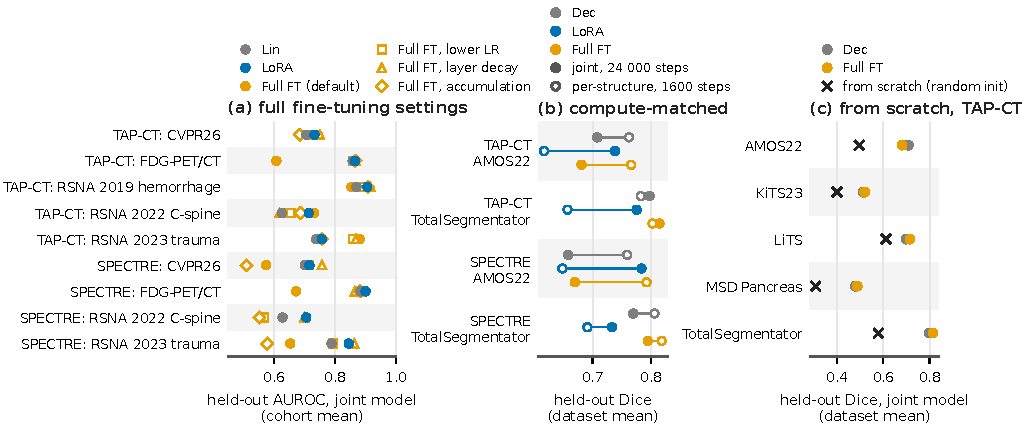
\includegraphics[width=\textwidth]{figures/fig_revision.pdf}
\caption{Repeats and controls. (a) Full fine-tuning settings against Lin and LoRA on the classification joint models. (b) Compute-matched segmentation: joint model against per-structure models at 1600 steps. (c) From-scratch control against Full FT and Dec on TAP-CT.}
\label{fig:revision}
\end{figure}

\begin{figure}[htbp]
\centering
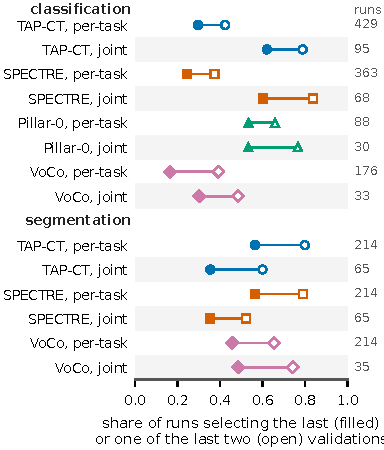
\includegraphics[width=\textwidth]{figures/fig_convergence.pdf}
\caption{Share of runs whose selected checkpoint is the last validation or one of the last two, per task and backbone.}
\label{fig:convergence}
\end{figure}

\begin{table}[htbp]
\centering
\caption{Convergence: share of runs that selected the last validation or one of the last two, per task and backbone.}
\label{tab:convergence}
\adjustbox{max width=\textwidth}{\small\begin{tabular}{@{}llrcc@{}}
\toprule
Backbone & Mode & Runs & \begin{tabular}[b]{@{}c@{}}Last validation\\{\scriptsize selected (\%)}\end{tabular} & \begin{tabular}[b]{@{}c@{}}One of last two\\{\scriptsize selected (\%)}\end{tabular} \\
\midrule
\multicolumn{5}{@{}l}{\textit{Classification}} \\
TAP-CT & per-task & 429 & 30 & 42 \\
 & joint & 120 & 64 & 79 \\
 & joint (26\,000 steps) & 11 & 9 & 9 \\
\addlinespace[2pt]
SPECTRE & per-task & 363 & 25 & 37 \\
 & joint & 88 & 56 & 78 \\
 & joint (26\,000 steps) & 11 & 18 & 27 \\
\addlinespace[2pt]
Pillar-0 & per-task & 88 & 53 & 66 \\
 & joint & 35 & 60 & 80 \\
\addlinespace[2pt]
VoCo & per-task & 176 & 16 & 39 \\
 & joint & 33 & 30 & 48 \\
\addlinespace[2pt]
All & all & 1354 & 33 & 49 \\
\addlinespace
\multicolumn{5}{@{}l}{\textit{Segmentation}} \\
TAP-CT & per-task & 214 & 57 & 80 \\
 & joint & 70 & 34 & 63 \\
 & joint (8000 steps) & 14 & 79 & 93 \\
 & per-task, compute-matched & 90 & 49 & 74 \\
\addlinespace[2pt]
SPECTRE & per-task & 214 & 57 & 79 \\
 & joint & 65 & 35 & 52 \\
 & joint (8000 steps) & 14 & 93 & 100 \\
 & per-task, compute-matched & 90 & 66 & 90 \\
\addlinespace[2pt]
VoCo & per-task & 214 & 46 & 65 \\
 & joint & 35 & 49 & 74 \\
 & joint (8000 steps) & 14 & 64 & 86 \\
\addlinespace[2pt]
All & all & 1034 & 52 & 75 \\
\bottomrule
\end{tabular}
}
\end{table}

\section{VoCo}
\label{app:voco}

\begin{table}[htbp]
\centering
\caption{The comparisons of Table~\ref{tab:key} on VoCo (\numLabelsVocoN{} labels from FDG-PET/CT, RSNA 2022 and RSNA 2023; all \numStructsVocoN{} structures).}
\label{tab:keyvoco}
\adjustbox{max width=\textwidth}{\small\begin{tabular}{@{}lcc@{}}
\toprule
Comparison & VoCo & Cohorts $>0$ \\
\midrule
\multicolumn{3}{@{}l}{\textit{Classification (AUROC)}} \\
LoRA $-$ Lin & \mci{-0.071}{-0.168}{-0.005} & 0/3 \\
LoRA $-$ Attn & \mci{-0.031}{-0.145}{+0.043} & 1/3 \\
Attn-only FT $-$ LoRA & \mci{+0.036}{-0.024}{+0.102} & 2/3 \\
Full FT $-$ Lin & \mci{-0.034}{-0.136}{+0.027} & 1/3 \\
joint $-$ per-task & \mci{-0.001}{-0.022}{+0.018} & 2/3 \\
\addlinespace
\multicolumn{3}{@{}l}{\textit{Segmentation (Dice)}} \\
Dec $-$ Lin & \mci{+0.680}{+0.433}{+0.746} & 5/5 \\
LoRA $-$ Dec & \mci{-0.018}{-0.047}{+0.016} & 2/5 \\
LoRA $-$ Dec, per-task & \mci{-0.035}{-0.062}{-0.007} & 0/5 \\
LoRA $-$ Dec, joint & \mci{0.000}{-0.034}{+0.047} & 2/5 \\
Full FT $-$ Dec & \mci{+0.015}{+0.007}{+0.023} & 4/5 \\
joint $-$ per-task & \mci{-0.041}{-0.081}{+0.004} & 2/5 \\
\bottomrule
\end{tabular}
}
\end{table}

\begin{table}[htbp]
\centering
\caption{VoCo classification: held-out AUROC as in Table~\ref{tab:cls}.}
\label{tab:clsvoco}
\adjustbox{max width=\textwidth}{\footnotesize\setlength{\tabcolsep}{3pt}
\begin{tabular}{@{}lllccccccccccc@{}}
\toprule
Cohort (labels) & Backbone & Mode & Lin & Attn & LoRA & LoRA$_{\text{late}}$ & \begin{tabular}[b]{@{}c@{}}LoRA+\\ABMIL\end{tabular} & DoRA & rsLoRA & \begin{tabular}[b]{@{}c@{}}Lin$\to$\\LoRA\end{tabular} & \begin{tabular}[b]{@{}c@{}}Attn$\to$\\LoRA\end{tabular} & \begin{tabular}[b]{@{}c@{}}Attn-only\\FT\end{tabular} & \begin{tabular}[b]{@{}c@{}}Full\\FT\end{tabular} \\
\midrule
FDG-PET/CT (4) & VoCo & per-task & \underline{0.720} & 0.685 & 0.512 & \cellcolor{modebest}0.671 & 0.562 & \cellcolor{modebest}0.669 & \cellcolor{modebest}0.598 & \textbf{0.736} & \cellcolor{modebest}0.591 & \cellcolor{modebest}0.665 & \cellcolor{modebest}0.606 \\
 &  & joint & \cellcolor{modebest}\underline{0.745} & \cellcolor{modebest}0.739 & \cellcolor{modebest}0.600 & 0.506 & \cellcolor{modebest}0.655 & 0.564 & 0.527 & \cellcolor{modebest}\textbf{0.750} & 0.520 & 0.641 & 0.582 \\
\addlinespace
RSNA 2022 C-spine (8) & VoCo & per-task & \cellcolor{modebest}\underline{0.606} & 0.508 & 0.537 & \cellcolor{modebest}0.551 & \cellcolor{modebest}0.596 & 0.561 & \cellcolor{modebest}\textbf{0.617} & 0.602 & 0.521 & 0.576 & \cellcolor{modebest}0.605 \\
 &  & joint & 0.586 & \cellcolor{modebest}0.548 & \cellcolor{modebest}0.560 & 0.550 & 0.565 & \cellcolor{modebest}0.589 & 0.578 & \cellcolor{modebest}\textbf{0.619} & \cellcolor{modebest}0.527 & \cellcolor{modebest}0.589 & \underline{0.593} \\
\addlinespace
RSNA 2023 trauma (4) & VoCo & per-task & 0.617 & \cellcolor{modebest}\underline{0.625} & \cellcolor{modebest}0.622 & 0.601 & \cellcolor{modebest}0.595 & \cellcolor{modebest}0.611 & \cellcolor{modebest}0.608 & \cellcolor{modebest}\textbf{0.631} & 0.569 & 0.588 & 0.596 \\
 &  & joint & \cellcolor{modebest}0.631 & 0.616 & 0.603 & \cellcolor{modebest}0.627 & 0.570 & 0.583 & 0.607 & 0.626 & \cellcolor{modebest}\underline{0.635} & \cellcolor{modebest}0.593 & \cellcolor{modebest}\textbf{0.648} \\
\bottomrule
\end{tabular}
}
\end{table}

\begin{table}[htbp]
\centering
\caption{VoCo segmentation: held-out Dice as in Table~\ref{tab:seg}.}
\label{tab:segvoco}
\adjustbox{max width=\textwidth}{\footnotesize\setlength{\tabcolsep}{3pt}
\begin{tabular}{@{}lllccccccc@{}}
\toprule
Dataset (structures) & Backbone & Mode & Lin & Dec & LoRA & LoRA$_{\text{late}}$ & DoRA & \begin{tabular}[b]{@{}c@{}}Full\\FT\end{tabular} & \begin{tabular}[b]{@{}c@{}}Dec$\to$\\LoRA\end{tabular} \\
\midrule
AMOS22 (15) & VoCo & per-task & \cellcolor{modebest}0.041 & \cellcolor{modebest}\underline{0.805} & \cellcolor{modebest}0.782 & \cellcolor{modebest}0.783 & \cellcolor{modebest}0.783 & \cellcolor{modebest}\textbf{0.818} & \cellcolor{modebest}0.799 \\
 &  & joint & 0.038 & 0.739 & \underline{0.762} & 0.758 & \textbf{0.764} & 0.752 & 0.736 \\
\addlinespace
KiTS23 (3) & VoCo & per-task & 0.017 & \cellcolor{modebest}\underline{0.519} & 0.501 & 0.500 & 0.493 & \cellcolor{modebest}\textbf{0.564} & \cellcolor{modebest}0.481 \\
 &  & joint & \cellcolor{modebest}0.037 & 0.465 & 0.501 & \cellcolor{modebest}\textbf{0.516} & \cellcolor{modebest}\underline{0.507} & 0.481 & 0.452 \\
\addlinespace
LiTS (2) & VoCo & per-task & 0.342 & \cellcolor{modebest}\underline{0.733} & 0.692 & 0.694 & 0.688 & \cellcolor{modebest}\textbf{0.748} & 0.720 \\
 &  & joint & \cellcolor{modebest}0.345 & \underline{0.732} & \cellcolor{modebest}0.720 & \cellcolor{modebest}0.710 & \cellcolor{modebest}0.718 & \textbf{0.737} & \cellcolor{modebest}0.726 \\
\addlinespace
MSD Pancreas (2) & VoCo & per-task & 0.000 & \cellcolor{modebest}\textbf{0.569} & 0.539 & 0.545 & 0.541 & \cellcolor{modebest}\underline{0.566} & 0.558 \\
 &  & joint & 0.000 & 0.559 & \cellcolor{modebest}0.552 & 0.545 & \cellcolor{modebest}0.552 & \underline{0.560} & \cellcolor{modebest}\textbf{0.561} \\
\addlinespace
TotalSegmentator (15) & VoCo & per-task & \cellcolor{modebest}0.055 & \cellcolor{modebest}\underline{0.822} & \cellcolor{modebest}0.771 & -- & -- & \cellcolor{modebest}\textbf{0.838} & -- \\
 &  & joint & 0.047 & \underline{0.732} & 0.705 & 0.697 & 0.709 & \textbf{0.750} & 0.723 \\
\bottomrule
\end{tabular}
}
\end{table}

\begin{figure}[htbp]
\centering
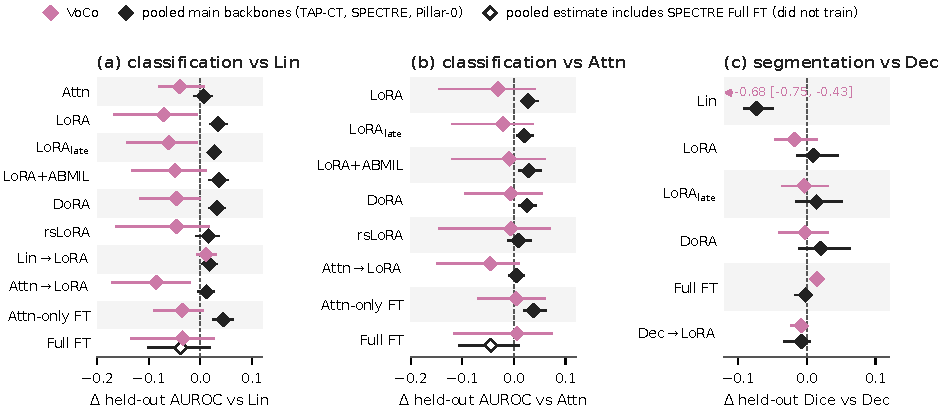
\includegraphics[width=\textwidth]{figures/fig_voco.pdf}
\caption{VoCo. (a) Label-level difference of every classification method to the linear probe on VoCo, next to the estimate pooled over the main backbones. (b) Per-structure change in held-out Dice relative to the frozen decoder on VoCo.}
\label{fig:voco}
\end{figure}

\begin{table}[htbp]
\centering
\caption{Median over label--mode pairs of the standard deviation of the held-out probabilities per backbone and method (the did-not-train rule flags values below \numSpreadMinValue{}; applied to TAP-CT, SPECTRE and Pillar-0 only).}
\label{tab:spread}
\adjustbox{max width=\textwidth}{\small\setlength{\tabcolsep}{3pt}
\begin{tabular}{lccccccccccc}
\toprule
Backbone & Lin & Attn & LoRA & LoRA$_{\text{late}}$ & LoRA+ABMIL & DoRA & rsLoRA & Lin$\to$LoRA & Attn$\to$LoRA & Attn-only FT & Full FT \\
\midrule
TAP-CT & 0.227 & 0.239 & 0.239 & 0.235 & 0.233 & 0.237 & 0.167 & 0.222 & 0.225 & 0.247 & 0.170 \\
SPECTRE & 0.187 & 0.114 & 0.161 & 0.185 & 0.187 & 0.185 & 0.150 & 0.178 & 0.129 & 0.148 & \textbf{0.004}$^{\dagger}$ \\
Pillar-0 & 0.294 & 0.321 & 0.359 & 0.350 & 0.352 & 0.354 & 0.359 & 0.337 & 0.338 & 0.355 & 0.347 \\
VoCo & 0.152 & 0.023 & 0.035 & 0.032 & 0.008 & 0.030 & 0.036 & 0.150 & 0.020 & 0.041 & 0.036 \\
\bottomrule
\end{tabular}
}
\end{table}

\section{Ranks, paired tests and per-label results}
\label{app:perlabel}

\begin{figure}[htbp]
\centering
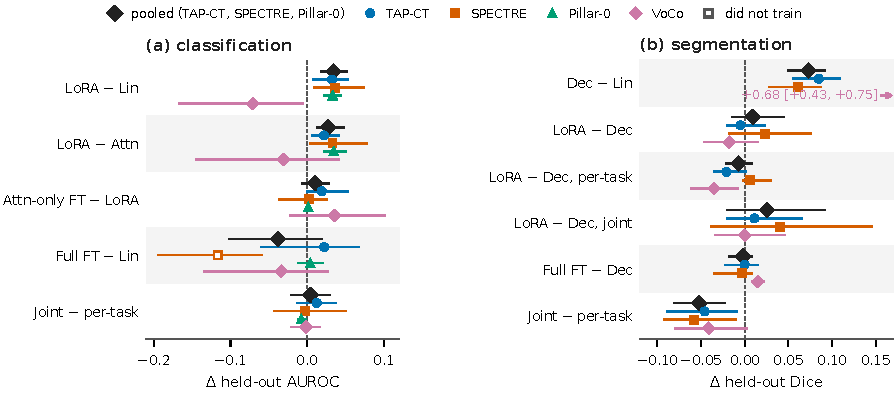
\includegraphics[width=\textwidth]{figures/fig_key.pdf}
\caption{The comparisons of Table~\ref{tab:key} per backbone: label-level mean difference in held-out AUROC (a) or Dice (b) with its 95\% interval; 0 means no difference. The black diamond pools TAP-CT, SPECTRE and Pillar-0; VoCo has its own marker and is never pooled.}
\label{fig:key}
\end{figure}

\begin{figure}[htbp]
\centering
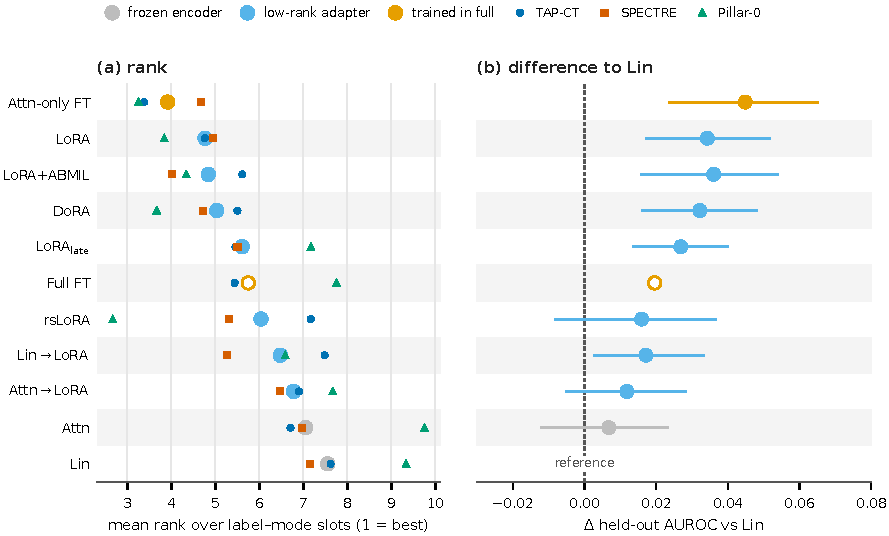
\includegraphics[width=\textwidth]{figures/fig_methods_cls_rank.pdf}
\caption{Classification methods on the three main backbones. (a) Mean rank over label--mode pairs, 1 = best; large markers pool the backbones, small markers are per backbone. (b) Label-level mean difference to the linear probe with its 95\% interval. SPECTRE Full FT, which did not train, is excluded from the ranks and drawn open in (b).}
\label{fig:ranks}
\end{figure}

\begin{figure}[htbp]
\centering
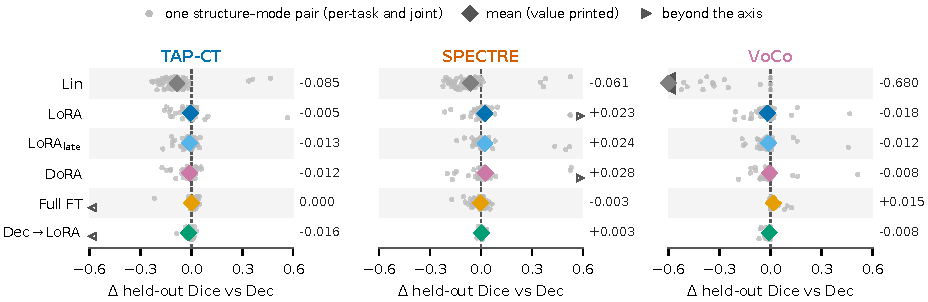
\includegraphics[width=\textwidth]{figures/fig_perstructure_seg.pdf}
\caption{Per-structure change in held-out Dice relative to the frozen decoder of the same backbone, dataset and mode (grey: structure--mode pairs; coloured: mean, printed on the right; open triangles: beyond the axis), for TAP-CT, SPECTRE and VoCo.}
\label{fig:perstructure}
\end{figure}

\begin{table}[htbp]
\centering
\caption{Classification: held-out AUROC, mean over the labels of each cohort (number of labels in brackets), per backbone, training mode and method. Best results are bolded, while second-best results are underlined. A \colorbox{modebest}{shaded} cell marks the better of per-task and joint training for that method, backbone and cohort. SPECTRE Full FT did not train with the default setting (Section~\ref{sec:fullft}) and is not marked.}
\label{tab:cls}
\adjustbox{max width=\textwidth}{\footnotesize\setlength{\tabcolsep}{3pt}
\begin{tabular}{@{}lllccccccccccc@{}}
\toprule
Cohort (labels) & Backbone & Mode & Lin & Attn & LoRA & LoRA$_{\text{late}}$ & \begin{tabular}[b]{@{}c@{}}LoRA+\\ABMIL\end{tabular} & DoRA & rsLoRA & \begin{tabular}[b]{@{}c@{}}Lin$\to$\\LoRA\end{tabular} & \begin{tabular}[b]{@{}c@{}}Attn$\to$\\LoRA\end{tabular} & \begin{tabular}[b]{@{}c@{}}Attn-only\\FT\end{tabular} & \begin{tabular}[b]{@{}c@{}}Full\\FT\end{tabular} \\
\midrule
CVPR26 (17) & TAP-CT & per-task & 0.677 & 0.718 & \underline{0.732} & 0.704 & 0.728 & 0.717 & \cellcolor{modebest}0.724 & \cellcolor{modebest}0.697 & 0.707 & \cellcolor{modebest}\textbf{0.744} & 0.720 \\
 &  & joint & \cellcolor{modebest}0.707 & \cellcolor{modebest}0.720 & \cellcolor{modebest}0.733 & \cellcolor{modebest}0.726 & \cellcolor{modebest}0.729 & \cellcolor{modebest}0.733 & 0.722 & 0.695 & \cellcolor{modebest}0.708 & \underline{0.739} & \cellcolor{modebest}\textbf{0.744} \\
\addlinespace[1.5pt]
 & SPECTRE & per-task & \cellcolor{modebest}0.736 & 0.725 & \cellcolor{modebest}0.769 & \cellcolor{modebest}0.769 & \cellcolor{modebest}\underline{0.776} & \cellcolor{modebest}0.766 & \cellcolor{modebest}0.768 & \cellcolor{modebest}0.769 & \cellcolor{modebest}0.765 & \cellcolor{modebest}\textbf{0.778} & 0.627$^{\dagger}$ \\
 &  & joint & 0.702 & \cellcolor{modebest}0.738 & 0.716 & 0.731 & \textbf{0.747} & 0.731 & 0.690 & \underline{0.744} & 0.728 & 0.740 & 0.575$^{\dagger}$ \\
\addlinespace
FDG-PET/CT (4) & TAP-CT & per-task & \cellcolor{modebest}0.863 & 0.836 & 0.852 & \cellcolor{modebest}\textbf{0.868} & 0.839 & 0.847 & \cellcolor{modebest}0.817 & \cellcolor{modebest}\underline{0.866} & 0.856 & 0.832 & \cellcolor{modebest}0.769 \\
 &  & joint & 0.858 & \cellcolor{modebest}0.860 & \cellcolor{modebest}\underline{0.866} & 0.864 & \cellcolor{modebest}0.849 & \cellcolor{modebest}0.858 & 0.785 & 0.860 & \cellcolor{modebest}0.862 & \cellcolor{modebest}\textbf{0.870} & 0.608 \\
\addlinespace[1.5pt]
 & SPECTRE & per-task & 0.857 & 0.862 & 0.882 & 0.879 & 0.874 & \textbf{0.892} & 0.872 & \cellcolor{modebest}\underline{0.887} & 0.867 & 0.848 & 0.617$^{\dagger}$ \\
 &  & joint & \cellcolor{modebest}0.884 & \cellcolor{modebest}0.880 & \cellcolor{modebest}\underline{0.901} & \cellcolor{modebest}0.888 & \cellcolor{modebest}0.889 & \cellcolor{modebest}0.900 & \cellcolor{modebest}0.900 & 0.884 & \cellcolor{modebest}0.884 & \cellcolor{modebest}\textbf{0.906} & 0.673$^{\dagger}$ \\
\addlinespace
RSNA 2022 C-spine (8) & TAP-CT & per-task & 0.619 & \cellcolor{modebest}0.625 & 0.623 & 0.608 & 0.613 & \underline{0.641} & \cellcolor{modebest}0.635 & 0.606 & \cellcolor{modebest}0.629 & \textbf{0.660} & 0.637 \\
 &  & joint & \cellcolor{modebest}0.626 & 0.624 & \cellcolor{modebest}\underline{0.714} & \cellcolor{modebest}0.706 & \cellcolor{modebest}0.713 & \cellcolor{modebest}0.680 & 0.601 & \cellcolor{modebest}0.624 & 0.620 & \cellcolor{modebest}0.712 & \cellcolor{modebest}\textbf{0.732} \\
\addlinespace[1.5pt]
 & SPECTRE & per-task & 0.579 & 0.591 & 0.635 & \cellcolor{modebest}\textbf{0.654} & \underline{0.644} & 0.619 & 0.638 & 0.615 & 0.591 & 0.635 & 0.566$^{\dagger}$ \\
 &  & joint & \cellcolor{modebest}0.629 & \cellcolor{modebest}0.601 & \cellcolor{modebest}0.706 & 0.644 & \cellcolor{modebest}\textbf{0.730} & \cellcolor{modebest}0.692 & \cellcolor{modebest}0.691 & \cellcolor{modebest}0.670 & \cellcolor{modebest}0.611 & \cellcolor{modebest}\underline{0.718} & 0.554$^{\dagger}$ \\
\addlinespace
RSNA 2023 trauma (4) & TAP-CT & per-task & 0.737 & 0.718 & 0.739 & \cellcolor{modebest}0.756 & 0.703 & 0.752 & \cellcolor{modebest}0.725 & 0.738 & 0.716 & \cellcolor{modebest}\textbf{0.859} & \underline{0.775} \\
 &  & joint & \cellcolor{modebest}0.739 & \cellcolor{modebest}0.738 & \cellcolor{modebest}0.757 & 0.744 & \cellcolor{modebest}0.758 & \cellcolor{modebest}0.768 & 0.684 & \cellcolor{modebest}0.746 & \cellcolor{modebest}0.758 & \underline{0.833} & \cellcolor{modebest}\textbf{0.881} \\
\addlinespace[1.5pt]
 & SPECTRE & per-task & \cellcolor{modebest}0.791 & 0.778 & 0.824 & 0.832 & \textbf{0.852} & \cellcolor{modebest}\underline{0.842} & 0.836 & 0.825 & 0.798 & 0.772 & 0.624$^{\dagger}$ \\
 &  & joint & 0.789 & \cellcolor{modebest}0.788 & \cellcolor{modebest}0.846 & \cellcolor{modebest}0.835 & \cellcolor{modebest}\textbf{0.859} & 0.838 & \cellcolor{modebest}\underline{0.850} & \cellcolor{modebest}0.827 & \cellcolor{modebest}0.810 & \cellcolor{modebest}0.803 & 0.654$^{\dagger}$ \\
\addlinespace
RSNA 2019 hemorrhage (6) & TAP-CT & per-task & 0.870 & 0.873 & 0.894 & 0.894 & \cellcolor{modebest}0.891 & \underline{0.897} & \cellcolor{modebest}0.870 & \cellcolor{modebest}0.877 & \cellcolor{modebest}0.878 & \textbf{0.911} & \cellcolor{modebest}0.888 \\
 &  & joint & \cellcolor{modebest}0.871 & \cellcolor{modebest}0.877 & \cellcolor{modebest}\underline{0.906} & \cellcolor{modebest}0.895 & 0.886 & 0.897 & 0.869 & 0.868 & 0.876 & \cellcolor{modebest}\textbf{0.915} & 0.854 \\
\addlinespace[1.5pt]
 & Pillar-0 & per-task & 0.886 & 0.884 & \cellcolor{modebest}\underline{0.929} & \cellcolor{modebest}0.914 & 0.902 & \cellcolor{modebest}\textbf{0.931} & \cellcolor{modebest}0.920 & \cellcolor{modebest}0.912 & \cellcolor{modebest}0.903 & \cellcolor{modebest}\textbf{0.931} & \cellcolor{modebest}0.904 \\
 &  & joint & \cellcolor{modebest}0.888 & \cellcolor{modebest}0.888 & 0.912 & 0.892 & \cellcolor{modebest}\textbf{0.925} & 0.912 & \underline{0.918} & 0.905 & 0.898 & 0.912 & 0.878 \\
\bottomrule
\end{tabular}
}
\end{table}

\begin{figure}[htbp]
\centering
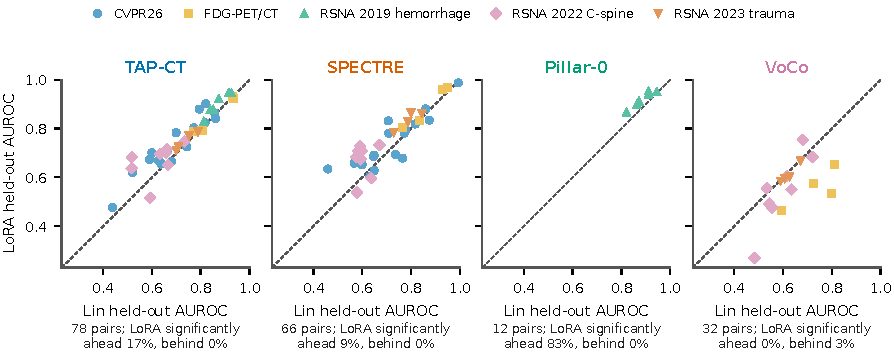
\includegraphics[width=\textwidth]{figures/fig_perlabel_cls.pdf}
\caption{Held-out AUROC of LoRA against the linear probe per label and mode, one panel per backbone; points above the identity line favour LoRA. The text under each panel gives the share of label--mode pairs in which LoRA is significantly ahead or behind.}
\label{fig:perlabel}
\end{figure}

\begin{table}[htbp]
\centering
\caption{Segmentation: held-out Dice, mean over the structures of each dataset (number of structures in brackets), per backbone, training mode and method; -- marks methods not run per structure on TotalSegmentator. Best results are bolded, while second-best results are underlined. A \colorbox{modebest}{shaded} cell marks the better of per-structure and joint training for that method, backbone and dataset. The AMOS22 and TotalSegmentator joint models train 24\,000 steps; their 8000-step runs are in Table~\ref{tab:segmodes}.}
\label{tab:seg}
\adjustbox{max width=\textwidth}{\footnotesize\setlength{\tabcolsep}{3pt}
\begin{tabular}{@{}lllccccccc@{}}
\toprule
Dataset (structures) & Backbone & Mode & Lin & Dec & LoRA & LoRA$_{\text{late}}$ & DoRA & \begin{tabular}[b]{@{}c@{}}Full\\FT\end{tabular} & \begin{tabular}[b]{@{}c@{}}Dec$\to$\\LoRA\end{tabular} \\
\midrule
AMOS22 (15) & TAP-CT & per-task & \cellcolor{modebest}0.658 & \cellcolor{modebest}\underline{0.793} & \cellcolor{modebest}0.767 & \cellcolor{modebest}0.764 & \cellcolor{modebest}0.761 & \cellcolor{modebest}\textbf{0.805} & \cellcolor{modebest}0.791 \\
 &  & joint & 0.646 & \underline{0.708} & \textbf{0.739} & 0.698 & \underline{0.708} & 0.681 & 0.656 \\
\addlinespace[1.5pt]
 & SPECTRE & per-task & \cellcolor{modebest}0.683 & \cellcolor{modebest}0.808 & \cellcolor{modebest}\underline{0.812} & \cellcolor{modebest}0.806 & \cellcolor{modebest}\textbf{0.814} & \cellcolor{modebest}0.792 & \cellcolor{modebest}\textbf{0.814} \\
 &  & joint & 0.682 & 0.658 & \textbf{0.784} & 0.764 & \underline{0.775} & 0.669 & 0.664 \\
\addlinespace
KiTS23 (3) & TAP-CT & per-task & \cellcolor{modebest}0.531 & \cellcolor{modebest}0.584 & 0.563 & \cellcolor{modebest}0.567 & \cellcolor{modebest}0.563 & \cellcolor{modebest}\textbf{0.588} & \cellcolor{modebest}\underline{0.587} \\
 &  & joint & 0.430 & 0.514 & \cellcolor{modebest}\textbf{0.582} & 0.556 & \underline{0.560} & 0.519 & 0.500 \\
\addlinespace[1.5pt]
 & SPECTRE & per-task & \cellcolor{modebest}0.583 & \cellcolor{modebest}0.599 & \cellcolor{modebest}0.613 & \cellcolor{modebest}\underline{0.617} & \cellcolor{modebest}\textbf{0.622} & \cellcolor{modebest}0.528 & \cellcolor{modebest}0.603 \\
 &  & joint & 0.530 & 0.572 & \underline{0.588} & \underline{0.588} & \textbf{0.593} & 0.519 & 0.570 \\
\addlinespace
LiTS (2) & TAP-CT & per-task & \cellcolor{modebest}0.659 & \cellcolor{modebest}0.709 & \cellcolor{modebest}\textbf{0.716} & 0.709 & \cellcolor{modebest}\underline{0.714} & 0.710 & \cellcolor{modebest}\underline{0.714} \\
 &  & joint & 0.656 & 0.699 & \underline{0.715} & \cellcolor{modebest}\textbf{0.721} & 0.692 & \cellcolor{modebest}\underline{0.715} & 0.703 \\
\addlinespace[1.5pt]
 & SPECTRE & per-task & 0.688 & \underline{0.741} & \cellcolor{modebest}\textbf{0.756} & 0.723 & \cellcolor{modebest}\textbf{0.756} & \cellcolor{modebest}0.739 & 0.729 \\
 &  & joint & \cellcolor{modebest}0.696 & \cellcolor{modebest}0.742 & \textbf{0.753} & \cellcolor{modebest}0.736 & \underline{0.743} & 0.713 & \cellcolor{modebest}\underline{0.743} \\
\addlinespace
MSD Pancreas (2) & TAP-CT & per-task & \cellcolor{modebest}0.427 & \cellcolor{modebest}0.491 & \underline{0.504} & \cellcolor{modebest}0.501 & \cellcolor{modebest}0.502 & \cellcolor{modebest}\textbf{0.512} & \cellcolor{modebest}0.495 \\
 &  & joint & 0.334 & 0.480 & \cellcolor{modebest}\textbf{0.505} & 0.492 & \underline{0.493} & 0.487 & 0.468 \\
\addlinespace[1.5pt]
 & SPECTRE & per-task & \cellcolor{modebest}0.475 & \cellcolor{modebest}0.516 & \cellcolor{modebest}\textbf{0.563} & \cellcolor{modebest}0.538 & \cellcolor{modebest}\underline{0.557} & 0.516 & 0.518 \\
 &  & joint & 0.459 & 0.514 & \textbf{0.550} & 0.529 & \textbf{0.550} & \cellcolor{modebest}\underline{0.530} & \cellcolor{modebest}0.520 \\
\addlinespace
TotalSegmentator (15) & TAP-CT & per-task & \cellcolor{modebest}0.747 & \cellcolor{modebest}\textbf{0.843} & \cellcolor{modebest}0.819 & -- & -- & \cellcolor{modebest}\underline{0.832} & -- \\
 &  & joint & 0.740 & \underline{0.798} & 0.776 & 0.776 & 0.776 & \textbf{0.815} & 0.790 \\
\addlinespace[1.5pt]
 & SPECTRE & per-task & \cellcolor{modebest}0.731 & \cellcolor{modebest}\textbf{0.848} & \cellcolor{modebest}\textbf{0.848} & -- & -- & \cellcolor{modebest}\underline{0.838} & -- \\
 &  & joint & 0.722 & 0.770 & 0.733 & 0.752 & 0.736 & \textbf{0.795} & \underline{0.772} \\
\bottomrule
\end{tabular}
}
\end{table}

\begin{figure}[htbp]
\centering
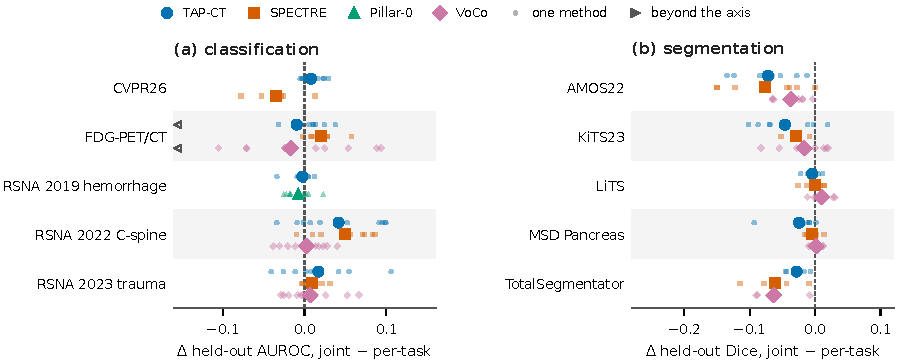
\includegraphics[width=\textwidth]{figures/fig_joint.pdf}
\caption{Joint minus per-task held-out AUROC per classification cohort (a) and joint minus per-structure held-out Dice per segmentation dataset (b), per backbone; small markers are methods, large markers their mean.}
\label{fig:joint}
\end{figure}

\begin{table}[htbp]
\centering
\caption{Classification: mean rank per method (1 = best) over the label--mode pairs with every method present, per backbone and pooled over the three main backbones; share of pairs within 0.01 AUROC of the best method and mean deficit to the best method.}
\label{tab:rankscls}
\adjustbox{max width=\textwidth}{\small\begin{tabular}{@{}lcccccc@{}}
\toprule
Method & \multicolumn{1}{c}{\begin{tabular}[b]{@{}c@{}}TAP-CT\\{\scriptsize 78 slots}\end{tabular}} & \multicolumn{1}{c}{\begin{tabular}[b]{@{}c@{}}SPECTRE\\{\scriptsize 66 slots}\end{tabular}} & \multicolumn{1}{c}{\begin{tabular}[b]{@{}c@{}}Pillar-0\\{\scriptsize 12 slots}\end{tabular}} & \multicolumn{1}{c}{\begin{tabular}[b]{@{}c@{}}All\\{\scriptsize 156 slots}\end{tabular}} & \begin{tabular}[b]{@{}c@{}}Within 0.01\\{\scriptsize of best (\%)}\end{tabular} & \begin{tabular}[b]{@{}c@{}}Regret\\{\scriptsize all}\end{tabular} \\
\midrule
Lin & 7.62 & 7.15 & 9.33 & 7.55 & 7 & 0.081 \\
Attn & 6.71 & 6.96 & 9.75 & 7.05 & 10 & 0.074 \\
LoRA & 4.76 & 4.94 & 3.83 & 4.76 & 23 & 0.046 \\
LoRA$_{\text{late}}$ & 5.46 & 5.50 & 7.17 & 5.61 & 17 & 0.054 \\
LoRA+ABMIL & 5.61 & \textbf{4.02} & 4.33 & 4.84 & 26 & 0.045 \\
DoRA & 5.50 & 4.72 & 3.67 & 5.03 & 19 & 0.049 \\
rsLoRA & 7.17 & 5.31 & \textbf{2.67} & 6.04 & 18 & 0.065 \\
Lin$\to$LoRA & 7.48 & 5.27 & 6.58 & 6.47 & 11 & 0.064 \\
Attn$\to$LoRA & 6.90 & 6.47 & 7.67 & 6.78 & 13 & 0.069 \\
Attn-only FT & \textbf{3.38} & 4.67 & 3.25 & \textbf{3.91} & \textbf{38} & \textbf{0.036} \\
Full FT & 5.44 & --$^{\dagger}$ & 7.75 & 5.74$^{\dagger}$ & 31 & 0.055 \\
\bottomrule
\end{tabular}
}
\end{table}

\begin{table}[htbp]
\centering
\caption{Segmentation: mean rank per method over the structure--mode pairs with all seven methods, per backbone and pooled.}
\label{tab:ranksseg}
\adjustbox{max width=\textwidth}{\small\begin{tabular}{@{}lccccc@{}}
\toprule
Method & \multicolumn{1}{c}{\begin{tabular}[b]{@{}c@{}}TAP-CT\\{\scriptsize 59 slots}\end{tabular}} & \multicolumn{1}{c}{\begin{tabular}[b]{@{}c@{}}SPECTRE\\{\scriptsize 59 slots}\end{tabular}} & \multicolumn{1}{c}{\begin{tabular}[b]{@{}c@{}}All\\{\scriptsize 118 slots}\end{tabular}} & \begin{tabular}[b]{@{}c@{}}Within 0.01\\{\scriptsize of best (\%)}\end{tabular} & \begin{tabular}[b]{@{}c@{}}Regret\\{\scriptsize all}\end{tabular} \\
\midrule
Lin & 6.49 & 6.25 & 6.37 & 4 & 0.116 \\
Dec & 3.70 & 4.35 & 4.03 & 21 & 0.051 \\
LoRA & 3.38 & 3.06 & 3.22 & 47 & \textbf{0.037} \\
LoRA$_{\text{late}}$ & 4.03 & 3.92 & 3.97 & 31 & 0.046 \\
DoRA & 3.91 & \textbf{2.86} & 3.38 & 44 & 0.043 \\
Full FT & \textbf{2.05} & 3.84 & \textbf{2.94} & \textbf{64} & 0.051 \\
Dec$\to$LoRA & 4.44 & 3.72 & 4.08 & 24 & 0.058 \\
\bottomrule
\end{tabular}
}
\end{table}

\begin{figure}[htbp]
\centering
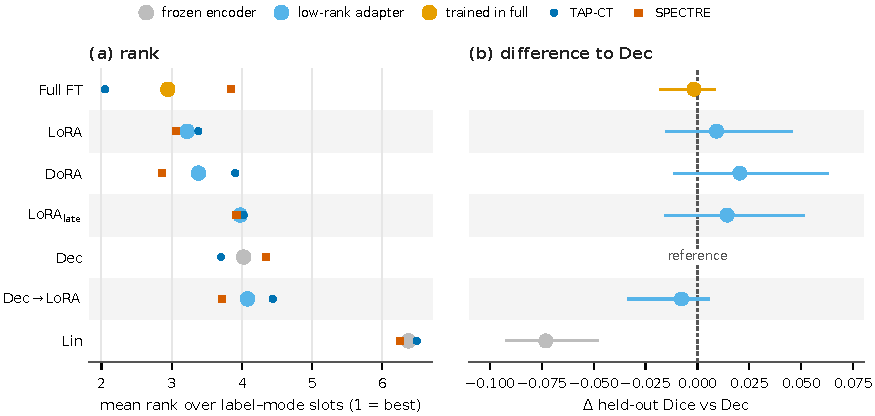
\includegraphics[width=\textwidth]{figures/fig_methods_seg_rank.pdf}
\caption{Segmentation methods on TAP-CT and SPECTRE. (a) Mean rank over structure--mode pairs, 1 = best. (b) Label-level mean difference to the frozen decoder with its 95\% interval.}
\label{fig:segranks}
\end{figure}

\begin{table}[htbp]
\centering
\caption{Label-level estimates for every comparison and backbone: number of labels, mean difference, 95\% interval over cohorts and labels, 95\% interval over cohorts, labels and held-out cases, and cohort--backbone clusters with a positive mean.}
\label{tab:cis}
\adjustbox{max width=\textwidth}{\footnotesize\begin{tabular}{@{}llrrccc@{}}
\toprule
Comparison & Backbone & $n$ & Mean & 95\% CI (two-stage) & 95\% CI (three-stage) & Cohorts $>0$ \\
\midrule
LoRA $-$ Lin & TAP-CT & 39 & +0.032 & [+0.009, +0.049] & [+0.007, +0.053] & 4/5 \\
 & SPECTRE & 33 & +0.037 & [+0.013, +0.068] & [+0.009, +0.075] & 4/4 \\
 & Pillar-0 & 6 & +0.033 & [+0.021, +0.042] & [+0.021, +0.044] & 1/1 \\
 & VoCo & 16 & -0.071 & [-0.162, -0.011] & [-0.168, -0.005] & 0/3 \\
 & All & 78 & +0.034 & [+0.019, +0.049] & [+0.017, +0.052] & 9/10 \\
\addlinespace[2pt]
LoRA $-$ Attn & TAP-CT & 39 & +0.022 & [+0.009, +0.039] & [+0.006, +0.042] & 5/5 \\
 & SPECTRE & 33 & +0.033 & [+0.007, +0.074] & [+0.003, +0.078] & 4/4 \\
 & Pillar-0 & 6 & +0.034 & [+0.021, +0.051] & [+0.021, +0.052] & 1/1 \\
 & VoCo & 16 & -0.031 & [-0.150, +0.033] & [-0.145, +0.043] & 1/3 \\
 & All & 78 & +0.027 & [+0.013, +0.047] & [+0.012, +0.048] & 10/10 \\
\addlinespace[2pt]
Attn-only FT $-$ LoRA & TAP-CT & 39 & +0.019 & [+0.002, +0.053] & [-0.001, +0.054] & 4/5 \\
 & SPECTRE & 33 & +0.002 & [-0.037, +0.023] & [-0.037, +0.026] & 2/4 \\
 & Pillar-0 & 6 & +0.001 & [0.000, +0.003] & [-0.002, +0.004] & 1/1 \\
 & VoCo & 16 & +0.036 & [-0.020, +0.097] & [-0.024, +0.102] & 2/3 \\
 & All & 78 & +0.011 & [-0.005, +0.026] & [-0.007, +0.029] & 7/10 \\
\addlinespace[2pt]
Full FT $-$ Lin & TAP-CT & 39 & +0.022 & [-0.057, +0.064] & [-0.061, +0.068] & 4/5 \\
 & SPECTRE & 33 & -0.117 & [-0.195, -0.063] & [-0.195, -0.059] & 0/4 \\
 & Pillar-0 & 6 & +0.004 & [-0.011, +0.019] & [-0.013, +0.021] & 1/1 \\
 & VoCo & 16 & -0.034 & [-0.133, +0.018] & [-0.136, +0.027] & 1/3 \\
 & All & 78 & -0.038 & [-0.101, +0.017] & [-0.103, +0.019] & 5/10 \\
\addlinespace[2pt]
joint $-$ per-task & TAP-CT & 39 & +0.012 & [-0.005, +0.032] & [-0.014, +0.038] & 3/5 \\
 & SPECTRE & 33 & -0.003 & [-0.035, +0.049] & [-0.044, +0.051] & 3/4 \\
 & Pillar-0 & 6 & -0.008 & [-0.012, -0.003] & [-0.013, -0.001] & 0/1 \\
 & VoCo & 16 & -0.001 & [-0.017, +0.012] & [-0.022, +0.018] & 2/3 \\
 & All & 78 & +0.004 & [-0.017, +0.027] & [-0.021, +0.030] & 6/10 \\
\addlinespace[2pt]
Attn $-$ Lin & TAP-CT & 39 & +0.011 & [-0.013, +0.027] & [-0.014, +0.029] & 3/5 \\
 & SPECTRE & 33 & +0.004 & [-0.022, +0.030] & [-0.030, +0.035] & 2/4 \\
 & Pillar-0 & 6 & -0.001 & [-0.012, +0.007] & [-0.014, +0.008] & 0/1 \\
 & VoCo & 16 & -0.040 & [-0.072, 0.000] & [-0.081, +0.008] & 0/3 \\
 & All & 78 & +0.007 & [-0.010, +0.021] & [-0.012, +0.023] & 5/10 \\
\addlinespace[2pt]
LoRA$_{\text{late}}$ $-$ Lin & TAP-CT & 39 & +0.023 & [+0.009, +0.036] & [+0.005, +0.039] & 5/5 \\
 & SPECTRE & 33 & +0.034 & [+0.016, +0.051] & [+0.011, +0.058] & 4/4 \\
 & Pillar-0 & 6 & +0.016 & [+0.008, +0.024] & [+0.007, +0.025] & 1/1 \\
 & VoCo & 16 & -0.061 & [-0.130, -0.010] & [-0.143, -0.005] & 0/3 \\
 & All & 78 & +0.027 & [+0.016, +0.038] & [+0.013, +0.040] & 10/10 \\
\addlinespace[2pt]
LoRA+ABMIL $-$ Lin & TAP-CT & 39 & +0.024 & [-0.006, +0.042] & [-0.005, +0.045] & 3/5 \\
 & SPECTRE & 33 & +0.052 & [+0.025, +0.080] & [+0.022, +0.086] & 4/4 \\
 & Pillar-0 & 6 & +0.026 & [+0.016, +0.037] & [+0.015, +0.038] & 1/1 \\
 & VoCo & 16 & -0.049 & [-0.134, -0.001] & [-0.134, +0.012] & 0/3 \\
 & All & 78 & +0.036 & [+0.018, +0.052] & [+0.016, +0.054] & 8/10 \\
\addlinespace[2pt]
DoRA $-$ Lin & TAP-CT & 39 & +0.028 & [+0.009, +0.042] & [+0.005, +0.046] & 4/5 \\
 & SPECTRE & 33 & +0.037 & [+0.014, +0.059] & [+0.009, +0.067] & 4/4 \\
 & Pillar-0 & 6 & +0.034 & [+0.021, +0.045] & [+0.020, +0.047] & 1/1 \\
 & VoCo & 16 & -0.046 & [-0.112, -0.011] & [-0.119, 0.000] & 0/3 \\
 & All & 78 & +0.032 & [+0.019, +0.045] & [+0.016, +0.048] & 9/10 \\
\addlinespace[2pt]
rsLoRA $-$ Lin & TAP-CT & 39 & +0.003 & [-0.043, +0.029] & [-0.043, +0.031] & 1/5 \\
 & SPECTRE & 33 & +0.028 & [+0.004, +0.063] & [0.000, +0.070] & 4/4 \\
 & Pillar-0 & 6 & +0.032 & [+0.021, +0.041] & [+0.020, +0.043] & 1/1 \\
 & VoCo & 16 & -0.046 & [-0.163, +0.006] & [-0.165, +0.018] & 1/3 \\
 & All & 78 & +0.016 & [-0.007, +0.035] & [-0.008, +0.037] & 6/10 \\
\addlinespace[2pt]
Lin$\to$LoRA $-$ Lin & TAP-CT & 39 & +0.001 & [-0.006, +0.007] & [-0.008, +0.010] & 4/5 \\
 & SPECTRE & 33 & +0.035 & [+0.018, +0.050] & [+0.012, +0.055] & 4/4 \\
 & Pillar-0 & 6 & +0.022 & [+0.013, +0.029] & [+0.013, +0.030] & 1/1 \\
 & VoCo & 16 & +0.011 & [-0.002, +0.025] & [-0.008, +0.031] & 3/3 \\
 & All & 78 & +0.017 & [+0.004, +0.032] & [+0.003, +0.034] & 9/10 \\
\addlinespace[2pt]
Attn$\to$LoRA $-$ Lin & TAP-CT & 39 & +0.008 & [-0.009, +0.019] & [-0.011, +0.024] & 3/5 \\
 & SPECTRE & 33 & +0.016 & [-0.014, +0.041] & [-0.017, +0.046] & 3/4 \\
 & Pillar-0 & 6 & +0.013 & [+0.007, +0.020] & [+0.006, +0.021] & 1/1 \\
 & VoCo & 16 & -0.086 & [-0.171, -0.022] & [-0.172, -0.018] & 0/3 \\
 & All & 78 & +0.012 & [-0.003, +0.026] & [-0.005, +0.028] & 7/10 \\
\addlinespace[2pt]
Attn-only FT $-$ Lin & TAP-CT & 39 & +0.051 & [+0.026, +0.078] & [+0.023, +0.080] & 4/5 \\
 & SPECTRE & 33 & +0.039 & [-0.001, +0.067] & [-0.003, +0.075] & 3/4 \\
 & Pillar-0 & 6 & +0.034 & [+0.022, +0.044] & [+0.021, +0.046] & 1/1 \\
 & VoCo & 16 & -0.035 & [-0.081, -0.008] & [-0.090, +0.007] & 0/3 \\
 & All & 78 & +0.045 & [+0.027, +0.062] & [+0.024, +0.065] & 8/10 \\
\addlinespace[2pt]
cls\_lorag\_attn & TAP-CT & 39 & +0.012 & [-0.002, +0.030] & [-0.004, +0.033] & 4/5 \\
 & SPECTRE & 33 & +0.030 & [+0.009, +0.058] & [+0.004, +0.063] & 4/4 \\
 & Pillar-0 & 6 & +0.017 & [+0.009, +0.028] & [+0.008, +0.029] & 1/1 \\
 & VoCo & 16 & -0.021 & [-0.116, +0.033] & [-0.121, +0.038] & 1/3 \\
 & All & 78 & +0.020 & [+0.007, +0.037] & [+0.005, +0.039] & 9/10 \\
\addlinespace[2pt]
cls\_babmil\_attn & TAP-CT & 39 & +0.014 & [-0.003, +0.032] & [-0.005, +0.035] & 4/5 \\
 & SPECTRE & 33 & +0.048 & [+0.018, +0.090] & [+0.014, +0.094] & 4/4 \\
 & Pillar-0 & 6 & +0.028 & [+0.018, +0.039] & [+0.018, +0.040] & 1/1 \\
 & VoCo & 16 & -0.009 & [-0.116, +0.058] & [-0.120, +0.062] & 1/3 \\
 & All & 78 & +0.029 & [+0.011, +0.052] & [+0.010, +0.055] & 9/10 \\
\addlinespace[2pt]
cls\_dora\_attn & TAP-CT & 39 & +0.017 & [+0.002, +0.036] & [-0.001, +0.038] & 5/5 \\
 & SPECTRE & 33 & +0.033 & [+0.013, +0.062] & [+0.009, +0.068] & 4/4 \\
 & Pillar-0 & 6 & +0.035 & [+0.020, +0.055] & [+0.020, +0.057] & 1/1 \\
 & VoCo & 16 & -0.006 & [-0.093, +0.050] & [-0.096, +0.056] & 1/3 \\
 & All & 78 & +0.025 & [+0.012, +0.042] & [+0.010, +0.044] & 10/10 \\
\addlinespace[2pt]
cls\_rslora\_attn & TAP-CT & 39 & -0.008 & [-0.036, +0.010] & [-0.039, +0.014] & 1/5 \\
 & SPECTRE & 33 & +0.024 & [-0.007, +0.072] & [-0.011, +0.078] & 3/4 \\
 & Pillar-0 & 6 & +0.033 & [+0.024, +0.042] & [+0.023, +0.044] & 1/1 \\
 & VoCo & 16 & -0.006 & [-0.144, +0.069] & [-0.146, +0.072] & 1/3 \\
 & All & 78 & +0.009 & [-0.009, +0.033] & [-0.013, +0.034] & 5/10 \\
\addlinespace[2pt]
cls\_attn\_then\_lorag\_attn & TAP-CT & 39 & -0.003 & [-0.013, +0.012] & [-0.016, +0.014] & 4/5 \\
 & SPECTRE & 33 & +0.012 & [-0.011, +0.032] & [-0.019, +0.037] & 4/4 \\
 & Pillar-0 & 6 & +0.014 & [+0.008, +0.025] & [+0.007, +0.026] & 1/1 \\
 & VoCo & 16 & -0.046 & [-0.150, +0.004] & [-0.151, +0.011] & 0/3 \\
 & All & 78 & +0.005 & [-0.007, +0.018] & [-0.010, +0.021] & 9/10 \\
\addlinespace[2pt]
cls\_attnft\_attn & TAP-CT & 39 & +0.041 & [+0.018, +0.078] & [+0.014, +0.082] & 5/5 \\
 & SPECTRE & 33 & +0.035 & [+0.001, +0.069] & [-0.002, +0.075] & 4/4 \\
 & Pillar-0 & 6 & +0.036 & [+0.022, +0.052] & [+0.021, +0.053] & 1/1 \\
 & VoCo & 16 & +0.005 & [-0.063, +0.053] & [-0.070, +0.061] & 1/3 \\
 & All & 78 & +0.038 & [+0.020, +0.060] & [+0.018, +0.062] & 10/10 \\
\addlinespace[2pt]
cls\_fullft\_attn & TAP-CT & 39 & +0.011 & [-0.056, +0.060] & [-0.058, +0.060] & 3/5 \\
 & SPECTRE & 33 & -0.121 & [-0.192, -0.059] & [-0.196, -0.054] & 0/4 \\
 & Pillar-0 & 6 & +0.005 & [-0.009, +0.017] & [-0.011, +0.019] & 1/1 \\
 & VoCo & 16 & +0.006 & [-0.115, +0.070] & [-0.118, +0.075] & 2/3 \\
 & All & 78 & -0.045 & [-0.105, +0.012] & [-0.108, +0.010] & 4/10 \\
\addlinespace[2pt]
cls\_lora\_lin\_nosc & TAP-CT & 34 & +0.035 & [+0.016, +0.053] & [+0.013, +0.056] & 4/4 \\
 & SPECTRE & 28 & +0.041 & [+0.015, +0.078] & [+0.009, +0.085] & 3/3 \\
 & Pillar-0 & 6 & +0.033 & [+0.021, +0.042] & [+0.020, +0.044] & 1/1 \\
 & VoCo & 12 & -0.036 & [-0.080, -0.006] & [-0.094, +0.011] & 0/2 \\
 & All & 68 & +0.037 & [+0.023, +0.054] & [+0.019, +0.057] & 8/8 \\
\bottomrule
\end{tabular}
}\\[6pt]
\adjustbox{max width=\textwidth}{\footnotesize\begin{tabular}{@{}llrrccc@{}}
\toprule
Comparison & Backbone & $n$ & Mean & 95\% CI (two-stage) & 95\% CI (three-stage) & Cohorts $>0$ \\
\midrule
Dec $-$ Lin & TAP-CT & 37 & +0.085 & [+0.055, +0.109] & [+0.055, +0.109] & 5/5 \\
 & SPECTRE & 37 & +0.061 & [+0.028, +0.089] & [+0.027, +0.088] & 5/5 \\
 & VoCo & 37 & +0.680 & [+0.430, +0.747] & [+0.433, +0.746] & 5/5 \\
 & All & 74 & +0.073 & [+0.049, +0.093] & [+0.049, +0.092] & 10/10 \\
\addlinespace[2pt]
LoRA $-$ Dec & TAP-CT & 37 & -0.005 & [-0.021, +0.023] & [-0.021, +0.024] & 4/5 \\
 & SPECTRE & 37 & +0.023 & [-0.017, +0.079] & [-0.018, +0.076] & 4/5 \\
 & VoCo & 37 & -0.018 & [-0.045, +0.017] & [-0.047, +0.016] & 2/5 \\
 & All & 74 & +0.009 & [-0.014, +0.046] & [-0.015, +0.046] & 8/10 \\
\addlinespace[2pt]
LoRA $-$ Dec, per-task & TAP-CT & 37 & -0.021 & [-0.035, +0.002] & [-0.036, +0.002] & 2/5 \\
 & SPECTRE & 37 & +0.006 & [-0.001, +0.028] & [-0.003, +0.031] & 5/5 \\
 & VoCo & 37 & -0.035 & [-0.062, -0.008] & [-0.062, -0.007] & 0/5 \\
 & All & 74 & -0.007 & [-0.021, +0.009] & [-0.022, +0.009] & 7/10 \\
\addlinespace[2pt]
LoRA $-$ Dec, joint & TAP-CT & 37 & +0.011 & [-0.019, +0.067] & [-0.021, +0.066] & 4/5 \\
 & SPECTRE & 37 & +0.040 & [-0.038, +0.148] & [-0.039, +0.147] & 4/5 \\
 & VoCo & 37 & 0.000 & [-0.034, +0.047] & [-0.034, +0.047] & 2/5 \\
 & All & 74 & +0.026 & [-0.020, +0.092] & [-0.021, +0.093] & 8/10 \\
\addlinespace[2pt]
Full FT $-$ Dec & TAP-CT & 37 & 0.000 & [-0.025, +0.015] & [-0.024, +0.016] & 4/5 \\
 & SPECTRE & 37 & -0.003 & [-0.033, +0.008] & [-0.035, +0.009] & 2/5 \\
 & VoCo & 37 & +0.015 & [+0.008, +0.023] & [+0.007, +0.023] & 4/5 \\
 & All & 74 & -0.002 & [-0.017, +0.009] & [-0.018, +0.009] & 6/10 \\
\addlinespace[2pt]
joint $-$ per-task & TAP-CT & 37 & -0.046 & [-0.088, -0.009] & [-0.090, -0.008] & 0/5 \\
 & SPECTRE & 37 & -0.058 & [-0.092, -0.010] & [-0.093, -0.009] & 0/5 \\
 & VoCo & 37 & -0.041 & [-0.081, +0.002] & [-0.081, +0.004] & 2/5 \\
 & All & 74 & -0.052 & [-0.082, -0.021] & [-0.082, -0.022] & 0/10 \\
\addlinespace[2pt]
Lin $-$ Dec & TAP-CT & 37 & -0.085 & [-0.109, -0.054] & [-0.110, -0.055] & 0/5 \\
 & SPECTRE & 37 & -0.061 & [-0.088, -0.027] & [-0.087, -0.027] & 0/5 \\
 & VoCo & 37 & -0.680 & [-0.746, -0.439] & [-0.745, -0.435] & 0/5 \\
 & All & 74 & -0.073 & [-0.092, -0.048] & [-0.093, -0.048] & 0/10 \\
\addlinespace[2pt]
LoRA$_{\text{late}}$ $-$ Dec & TAP-CT & 22 & -0.010 & [-0.023, +0.014] & [-0.024, +0.018] & 3/4 \\
 & SPECTRE & 22 & +0.038 & [-0.008, +0.073] & [-0.009, +0.071] & 3/4 \\
 & VoCo & 22 & -0.004 & [-0.037, +0.033] & [-0.037, +0.032] & 1/4 \\
 & All & 44 & +0.014 & [-0.015, +0.051] & [-0.016, +0.051] & 6/8 \\
\addlinespace[2pt]
DoRA $-$ Dec & TAP-CT & 22 & -0.008 & [-0.021, +0.013] & [-0.021, +0.015] & 2/4 \\
 & SPECTRE & 22 & +0.049 & [+0.008, +0.088] & [+0.006, +0.090] & 4/4 \\
 & VoCo & 22 & -0.002 & [-0.040, +0.033] & [-0.041, +0.032] & 2/4 \\
 & All & 44 & +0.020 & [-0.011, +0.063] & [-0.011, +0.063] & 6/8 \\
\addlinespace[2pt]
Dec$\to$LoRA $-$ Dec & TAP-CT & 22 & -0.019 & [-0.053, +0.006] & [-0.053, +0.007] & 1/4 \\
 & SPECTRE & 22 & +0.004 & [-0.005, +0.008] & [-0.007, +0.009] & 3/4 \\
 & VoCo & 22 & -0.008 & [-0.023, -0.004] & [-0.024, -0.003] & 0/4 \\
 & All & 44 & -0.008 & [-0.033, +0.005] & [-0.034, +0.006] & 4/8 \\
\bottomrule
\end{tabular}
}
\end{table}

\begin{table}[htbp]
\centering
\caption{Classification paired tests: share of label--mode pairs in which the method is ahead of the baseline, and significantly ahead or behind (DeLong, Benjamini--Hochberg, adjusted $p<0.05$), per backbone.}
\label{tab:pairedcls}
\adjustbox{max width=\textwidth}{\footnotesize\setlength{\tabcolsep}{3.5pt}
\begin{tabular}{@{}llrrrrrrrrrrrrrrrrr@{}}
\toprule
Backbone & Method & $n$ & \multicolumn{4}{c}{vs Lin} & \multicolumn{4}{c}{vs LoRA} & \multicolumn{4}{c}{vs Attn} & \multicolumn{4}{c}{vs Full FT} \\
\cmidrule(lr){4-7}\cmidrule(lr){8-11}\cmidrule(lr){12-15}\cmidrule(lr){16-19}
 & & & $\Delta$ & $>0$ & $+$ & $-$ & $\Delta$ & $>0$ & $+$ & $-$ & $\Delta$ & $>0$ & $+$ & $-$ & $\Delta$ & $>0$ & $+$ & $-$ \\
\midrule
TAP-CT & Lin & 78 & -- & -- & -- & -- & -0.032 & 22 & 0 & 17 & -0.011 & 41 & 0 & 4 & -0.022 & 28 & 12 & 17 \\
 & Attn & 78 & +0.011 & 59 & 4 & 0 & -0.022 & 36 & 0 & 15 & -- & -- & -- & -- & -0.011 & 40 & 10 & 18 \\
 & LoRA & 78 & +0.032 & 78 & 17 & 0 & -- & -- & -- & -- & +0.022 & 64 & 15 & 0 & +0.010 & 55 & 18 & 6 \\
 & LoRA$_{\text{late}}$ & 78 & +0.023 & 69 & 14 & 1 & -0.010 & 35 & 1 & 9 & +0.012 & 62 & 10 & 1 & +0.001 & 44 & 18 & 6 \\
 & LoRA+ABMIL & 78 & +0.024 & 68 & 12 & 1 & -0.008 & 47 & 4 & 13 & +0.014 & 60 & 12 & 1 & +0.002 & 45 & 17 & 12 \\
 & DoRA & 78 & +0.028 & 68 & 17 & 0 & -0.005 & 40 & 4 & 10 & +0.017 & 65 & 17 & 0 & +0.006 & 51 & 17 & 9 \\
 & rsLoRA & 78 & +0.003 & 55 & 5 & 5 & -0.029 & 28 & 1 & 23 & -0.008 & 44 & 5 & 6 & -0.019 & 47 & 13 & 22 \\
 & Lin$\to$LoRA & 78 & +0.001 & 51 & 5 & 1 & -0.031 & 28 & 0 & 17 & -0.009 & 44 & 3 & 4 & -0.021 & 31 & 9 & 18 \\
 & Attn$\to$LoRA & 78 & +0.008 & 56 & 9 & 0 & -0.024 & 28 & 0 & 17 & -0.003 & 47 & 3 & 0 & -0.014 & 38 & 13 & 15 \\
 & Attn-only FT & 78 & +0.051 & 83 & 24 & 0 & +0.019 & 64 & 17 & 0 & +0.041 & 81 & 26 & 0 & +0.029 & 63 & 23 & 5 \\
 & Full FT & 78 & +0.022 & 72 & 13 & 8 & -0.010 & 45 & 6 & 17 & +0.011 & 59 & 15 & 8 & -- & -- & -- & -- \\
\addlinespace
SPECTRE & Lin & 66 & -- & -- & -- & -- & -0.037 & 26 & 0 & 9 & -0.004 & 50 & 2 & 3 & -- & -- & -- & -- \\
 & Attn & 66 & +0.004 & 50 & 3 & 2 & -0.033 & 29 & 0 & 9 & -- & -- & -- & -- & -- & -- & -- & -- \\
 & LoRA & 66 & +0.037 & 74 & 9 & 0 & -- & -- & -- & -- & +0.033 & 71 & 9 & 0 & -- & -- & -- & -- \\
 & LoRA$_{\text{late}}$ & 66 & +0.034 & 65 & 5 & 0 & -0.003 & 47 & 2 & 2 & +0.030 & 67 & 9 & 0 & -- & -- & -- & -- \\
 & LoRA+ABMIL & 66 & +0.052 & 77 & 12 & 2 & +0.015 & 71 & 3 & 2 & +0.048 & 76 & 17 & 0 & -- & -- & -- & -- \\
 & DoRA & 66 & +0.037 & 77 & 8 & 0 & 0.000 & 50 & 2 & 3 & +0.033 & 71 & 9 & 0 & -- & -- & -- & -- \\
 & rsLoRA & 66 & +0.028 & 70 & 9 & 0 & -0.008 & 35 & 0 & 3 & +0.024 & 65 & 11 & 0 & -- & -- & -- & -- \\
 & Lin$\to$LoRA & 66 & +0.035 & 71 & 6 & 0 & -0.001 & 44 & 2 & 3 & +0.031 & 71 & 8 & 0 & -- & -- & -- & -- \\
 & Attn$\to$LoRA & 66 & +0.016 & 59 & 6 & 2 & -0.021 & 33 & 0 & 3 & +0.012 & 56 & 3 & 0 & -- & -- & -- & -- \\
 & Attn-only FT & 66 & +0.039 & 70 & 3 & 3 & +0.002 & 55 & 5 & 5 & +0.035 & 67 & 6 & 2 & -- & -- & -- & -- \\
 & Full FT$^{\dagger}$ & 66 & -0.117 & 21 & 0 & 32 & -0.153 & 6 & 0 & 39 & -0.121 & 14 & 0 & 32 & -- & -- & -- & -- \\
\addlinespace
Pillar-0 & Lin & 12 & -- & -- & -- & -- & -0.033 & 8 & 0 & 83 & +0.001 & 58 & 8 & 33 & -0.004 & 33 & 17 & 50 \\
 & Attn & 12 & -0.001 & 42 & 33 & 8 & -0.034 & 8 & 0 & 92 & -- & -- & -- & -- & -0.005 & 33 & 17 & 58 \\
 & LoRA & 12 & +0.033 & 92 & 83 & 0 & -- & -- & -- & -- & +0.034 & 92 & 92 & 0 & +0.029 & 100 & 67 & 0 \\
 & LoRA$_{\text{late}}$ & 12 & +0.016 & 75 & 67 & 0 & -0.017 & 0 & 0 & 83 & +0.017 & 75 & 67 & 8 & +0.012 & 58 & 33 & 25 \\
 & LoRA+ABMIL & 12 & +0.026 & 83 & 75 & 8 & -0.007 & 50 & 42 & 33 & +0.028 & 92 & 83 & 0 & +0.022 & 58 & 58 & 8 \\
 & DoRA & 12 & +0.034 & 92 & 83 & 0 & +0.001 & 50 & 0 & 8 & +0.035 & 100 & 92 & 0 & +0.030 & 83 & 67 & 0 \\
 & rsLoRA & 12 & +0.032 & 100 & 83 & 0 & -0.001 & 75 & 17 & 8 & +0.033 & 100 & 92 & 0 & +0.028 & 92 & 67 & 0 \\
 & Lin$\to$LoRA & 12 & +0.022 & 100 & 83 & 0 & -0.012 & 8 & 8 & 58 & +0.023 & 100 & 92 & 0 & +0.018 & 67 & 42 & 25 \\
 & Attn$\to$LoRA & 12 & +0.013 & 92 & 58 & 0 & -0.020 & 8 & 0 & 83 & +0.014 & 100 & 58 & 0 & +0.009 & 50 & 33 & 25 \\
 & Attn-only FT & 12 & +0.034 & 92 & 83 & 0 & +0.001 & 75 & 8 & 0 & +0.036 & 92 & 83 & 0 & +0.030 & 100 & 83 & 0 \\
 & Full FT & 12 & +0.004 & 67 & 50 & 17 & -0.029 & 0 & 0 & 67 & +0.005 & 67 & 42 & 8 & -- & -- & -- & -- \\
\bottomrule
\end{tabular}
}
\end{table}

\begin{table}[htbp]
\centering
\caption{Segmentation paired tests: share of structure--mode pairs in which the method is ahead of the baseline, and significantly ahead or behind (paired case bootstrap, Benjamini--Hochberg, adjusted $p<0.05$), per backbone.}
\label{tab:pairedseg}
\adjustbox{max width=\textwidth}{\footnotesize\setlength{\tabcolsep}{3.5pt}
\begin{tabular}{@{}llrrrrrrrrrrrrr@{}}
\toprule
Backbone & Method & $n$ & \multicolumn{4}{c}{vs Lin} & \multicolumn{4}{c}{vs Dec} & \multicolumn{4}{c}{vs LoRA} \\
\cmidrule(lr){4-7}\cmidrule(lr){8-11}\cmidrule(lr){12-15}
 & & & $\Delta$ & $>0$ & $+$ & $-$ & $\Delta$ & $>0$ & $+$ & $-$ & $\Delta$ & $>0$ & $+$ & $-$ \\
\midrule
TAP-CT & Lin & 74 & -- & -- & -- & -- & -0.086 & 4 & 4 & 93 & -0.088 & 4 & 3 & 93 \\
 & Dec & 74 & +0.086 & 96 & 93 & 4 & -- & -- & -- & -- & -0.002 & 43 & 30 & 31 \\
 & LoRA & 74 & +0.088 & 96 & 93 & 3 & +0.002 & 54 & 31 & 30 & -- & -- & -- & -- \\
 & LoRA$_{\text{late}}$ & 59 & +0.077 & 95 & 92 & 5 & -0.006 & 53 & 29 & 32 & -0.012 & 39 & 14 & 29 \\
 & DoRA & 59 & +0.078 & 95 & 90 & 5 & -0.006 & 53 & 25 & 25 & -0.011 & 34 & 10 & 31 \\
 & Full FT & 74 & +0.085 & 93 & 93 & 7 & -0.001 & 76 & 53 & 8 & -0.002 & 70 & 54 & 12 \\
 & Dec$\to$LoRA & 59 & +0.066 & 92 & 88 & 8 & -0.017 & 29 & 7 & 44 & -0.024 & 29 & 20 & 37 \\
\addlinespace
SPECTRE & Lin & 74 & -- & -- & -- & -- & -0.061 & 8 & 5 & 86 & -0.095 & 7 & 4 & 92 \\
 & Dec & 74 & +0.061 & 92 & 86 & 5 & -- & -- & -- & -- & -0.034 & 19 & 8 & 57 \\
 & LoRA & 74 & +0.095 & 93 & 93 & 4 & +0.034 & 80 & 57 & 8 & -- & -- & -- & -- \\
 & LoRA$_{\text{late}}$ & 59 & +0.079 & 92 & 90 & 5 & +0.032 & 69 & 46 & 8 & -0.009 & 27 & 8 & 42 \\
 & DoRA & 59 & +0.088 & 93 & 90 & 7 & +0.041 & 76 & 54 & 12 & +0.001 & 58 & 25 & 15 \\
 & Full FT & 74 & +0.059 & 89 & 81 & 8 & -0.002 & 54 & 38 & 20 & -0.035 & 36 & 27 & 31 \\
 & Dec$\to$LoRA & 59 & +0.051 & 90 & 85 & 7 & +0.004 & 69 & 20 & 12 & -0.037 & 25 & 10 & 49 \\
\bottomrule
\end{tabular}
}
\end{table}

\begin{table}[htbp]
\centering
\caption{Segmentation per mode: LoRA $-$ Dec and Full FT $-$ Dec in dataset-mean held-out Dice per backbone and mode, including the 8000-step joint models of AMOS22 and TotalSegmentator.}
\label{tab:segmodes}
\adjustbox{max width=\textwidth}{\footnotesize\begin{tabular}{@{}llcccccc@{}}
\toprule
Dataset (structures) & Backbone & \multicolumn{2}{c}{per-task} & \multicolumn{2}{c}{joint} & \multicolumn{2}{c}{joint, 8000 steps} \\
\cmidrule(lr){3-4}\cmidrule(lr){5-6}\cmidrule(lr){7-8}
 & & LoRA $-$ Dec & Full FT $-$ Dec & LoRA $-$ Dec & Full FT $-$ Dec & LoRA $-$ Dec & Full FT $-$ Dec \\
\midrule
AMOS22 (15) & TAP-CT & -0.026 & +0.012 & +0.031 & -0.027 & -0.125 & +0.007 \\
 & SPECTRE & +0.004 & -0.016 & +0.126 & +0.011 & -0.071 & +0.010 \\
\addlinespace
KiTS23 (3) & TAP-CT & -0.021 & +0.005 & +0.068 & +0.006 & -- & -- \\
 & SPECTRE & +0.014 & -0.071 & +0.016 & -0.052 & -- & -- \\
\addlinespace
LiTS (2) & TAP-CT & +0.007 & +0.001 & +0.016 & +0.016 & -- & -- \\
 & SPECTRE & +0.015 & -0.002 & +0.011 & -0.030 & -- & -- \\
\addlinespace
MSD Pancreas (2) & TAP-CT & +0.013 & +0.021 & +0.025 & +0.008 & -- & -- \\
 & SPECTRE & +0.047 & 0.000 & +0.037 & +0.016 & -- & -- \\
\addlinespace
TotalSegmentator (15) & TAP-CT & -0.024 & -0.011 & -0.022 & +0.017 & -0.199 & +0.022 \\
 & SPECTRE & +0.001 & -0.009 & -0.036 & +0.025 & -0.254 & +0.037 \\
\bottomrule
\end{tabular}
}
\end{table}

\begin{table}[htbp]
\centering
\caption{Held-out AUROC as in Table~\ref{tab:cls} for every backbone, with the 26\,000-step CVPR26 joint schedule as an extra row.}
\label{tab:clsladder}
\adjustbox{max width=\textwidth}{\footnotesize\setlength{\tabcolsep}{3pt}
\begin{tabular}{@{}lllccccccccccc@{}}
\toprule
Cohort (labels) & Backbone & Mode & Lin & Attn & LoRA & LoRA$_{\text{late}}$ & \begin{tabular}[b]{@{}c@{}}LoRA+\\ABMIL\end{tabular} & DoRA & rsLoRA & \begin{tabular}[b]{@{}c@{}}Lin$\to$\\LoRA\end{tabular} & \begin{tabular}[b]{@{}c@{}}Attn$\to$\\LoRA\end{tabular} & \begin{tabular}[b]{@{}c@{}}Attn-only\\FT\end{tabular} & \begin{tabular}[b]{@{}c@{}}Full\\FT\end{tabular} \\
\midrule
CVPR26 (17) & TAP-CT & per-task & 0.677 & 0.718 & \underline{0.732} & 0.704 & 0.728 & 0.717 & \cellcolor{modebest}0.724 & \cellcolor{modebest}0.697 & 0.707 & \cellcolor{modebest}\textbf{0.744} & 0.720 \\
 &  & joint & \cellcolor{modebest}0.707 & \cellcolor{modebest}0.720 & \cellcolor{modebest}0.733 & \cellcolor{modebest}0.726 & \cellcolor{modebest}0.729 & \cellcolor{modebest}0.733 & 0.722 & 0.695 & \cellcolor{modebest}0.708 & \underline{0.739} & \cellcolor{modebest}\textbf{0.744} \\
 &  & joint (26\,000 steps) & 0.693 & 0.722 & 0.692 & \underline{0.728} & 0.727 & 0.720 & 0.701 & 0.698 & 0.726 & \textbf{0.756} & 0.650 \\
\addlinespace[1.5pt]
 & SPECTRE & per-task & \cellcolor{modebest}0.736 & 0.725 & \cellcolor{modebest}0.769 & \cellcolor{modebest}0.769 & \cellcolor{modebest}\underline{0.776} & \cellcolor{modebest}0.766 & \cellcolor{modebest}0.768 & \cellcolor{modebest}0.769 & \cellcolor{modebest}0.765 & \cellcolor{modebest}\textbf{0.778} & 0.627$^{\dagger}$ \\
 &  & joint & 0.702 & \cellcolor{modebest}0.738 & 0.716 & 0.731 & \textbf{0.747} & 0.731 & 0.690 & \underline{0.744} & 0.728 & 0.740 & 0.575$^{\dagger}$ \\
 &  & joint (26\,000 steps) & 0.744 & 0.713 & 0.755 & \underline{0.762} & 0.760 & 0.752 & \textbf{0.763} & 0.746 & 0.758 & 0.756 & 0.574$^{\dagger}$ \\
\addlinespace
FDG-PET/CT (4) & TAP-CT & per-task & \cellcolor{modebest}0.863 & 0.836 & 0.852 & \cellcolor{modebest}\textbf{0.868} & 0.839 & 0.847 & \cellcolor{modebest}0.817 & \cellcolor{modebest}\underline{0.866} & 0.856 & 0.832 & \cellcolor{modebest}0.769 \\
 &  & joint & 0.858 & \cellcolor{modebest}0.860 & \cellcolor{modebest}\underline{0.866} & 0.864 & \cellcolor{modebest}0.849 & \cellcolor{modebest}0.858 & 0.785 & 0.860 & \cellcolor{modebest}0.862 & \cellcolor{modebest}\textbf{0.870} & 0.608 \\
\addlinespace[1.5pt]
 & SPECTRE & per-task & 0.857 & 0.862 & 0.882 & 0.879 & 0.874 & \textbf{0.892} & 0.872 & \cellcolor{modebest}\underline{0.887} & 0.867 & 0.848 & 0.617$^{\dagger}$ \\
 &  & joint & \cellcolor{modebest}0.884 & \cellcolor{modebest}0.880 & \cellcolor{modebest}\underline{0.901} & \cellcolor{modebest}0.888 & \cellcolor{modebest}0.889 & \cellcolor{modebest}0.900 & \cellcolor{modebest}0.900 & 0.884 & \cellcolor{modebest}0.884 & \cellcolor{modebest}\textbf{0.906} & 0.673$^{\dagger}$ \\
\addlinespace[1.5pt]
 & VoCo & per-task & \underline{0.720} & 0.685 & 0.512 & \cellcolor{modebest}0.671 & 0.562 & \cellcolor{modebest}0.669 & \cellcolor{modebest}0.598 & \textbf{0.736} & \cellcolor{modebest}0.591 & \cellcolor{modebest}0.665 & \cellcolor{modebest}0.606 \\
 &  & joint & \cellcolor{modebest}\underline{0.745} & \cellcolor{modebest}0.739 & \cellcolor{modebest}0.600 & 0.506 & \cellcolor{modebest}0.655 & 0.564 & 0.527 & \cellcolor{modebest}\textbf{0.750} & 0.520 & 0.641 & 0.582 \\
\addlinespace
RSNA 2022 C-spine (8) & TAP-CT & per-task & 0.619 & \cellcolor{modebest}0.625 & 0.623 & 0.608 & 0.613 & \underline{0.641} & \cellcolor{modebest}0.635 & 0.606 & \cellcolor{modebest}0.629 & \textbf{0.660} & 0.637 \\
 &  & joint & \cellcolor{modebest}0.626 & 0.624 & \cellcolor{modebest}\underline{0.714} & \cellcolor{modebest}0.706 & \cellcolor{modebest}0.713 & \cellcolor{modebest}0.680 & 0.601 & \cellcolor{modebest}0.624 & 0.620 & \cellcolor{modebest}0.712 & \cellcolor{modebest}\textbf{0.732} \\
\addlinespace[1.5pt]
 & SPECTRE & per-task & 0.579 & 0.591 & 0.635 & \cellcolor{modebest}\textbf{0.654} & \underline{0.644} & 0.619 & 0.638 & 0.615 & 0.591 & 0.635 & 0.566$^{\dagger}$ \\
 &  & joint & \cellcolor{modebest}0.629 & \cellcolor{modebest}0.601 & \cellcolor{modebest}0.706 & 0.644 & \cellcolor{modebest}\textbf{0.730} & \cellcolor{modebest}0.692 & \cellcolor{modebest}0.691 & \cellcolor{modebest}0.670 & \cellcolor{modebest}0.611 & \cellcolor{modebest}\underline{0.718} & 0.554$^{\dagger}$ \\
\addlinespace[1.5pt]
 & VoCo & per-task & \cellcolor{modebest}\underline{0.606} & 0.508 & 0.537 & \cellcolor{modebest}0.551 & \cellcolor{modebest}0.596 & 0.561 & \cellcolor{modebest}\textbf{0.617} & 0.602 & 0.521 & 0.576 & \cellcolor{modebest}0.605 \\
 &  & joint & 0.586 & \cellcolor{modebest}0.548 & \cellcolor{modebest}0.560 & 0.550 & 0.565 & \cellcolor{modebest}0.589 & 0.578 & \cellcolor{modebest}\textbf{0.619} & \cellcolor{modebest}0.527 & \cellcolor{modebest}0.589 & \underline{0.593} \\
\addlinespace
RSNA 2023 trauma (4) & TAP-CT & per-task & 0.737 & 0.718 & 0.739 & \cellcolor{modebest}0.756 & 0.703 & 0.752 & \cellcolor{modebest}0.725 & 0.738 & 0.716 & \cellcolor{modebest}\textbf{0.859} & \underline{0.775} \\
 &  & joint & \cellcolor{modebest}0.739 & \cellcolor{modebest}0.738 & \cellcolor{modebest}0.757 & 0.744 & \cellcolor{modebest}0.758 & \cellcolor{modebest}0.768 & 0.684 & \cellcolor{modebest}0.746 & \cellcolor{modebest}0.758 & \underline{0.833} & \cellcolor{modebest}\textbf{0.881} \\
\addlinespace[1.5pt]
 & SPECTRE & per-task & \cellcolor{modebest}0.791 & 0.778 & 0.824 & 0.832 & \textbf{0.852} & \cellcolor{modebest}\underline{0.842} & 0.836 & 0.825 & 0.798 & 0.772 & 0.624$^{\dagger}$ \\
 &  & joint & 0.789 & \cellcolor{modebest}0.788 & \cellcolor{modebest}0.846 & \cellcolor{modebest}0.835 & \cellcolor{modebest}\textbf{0.859} & 0.838 & \cellcolor{modebest}\underline{0.850} & \cellcolor{modebest}0.827 & \cellcolor{modebest}0.810 & \cellcolor{modebest}0.803 & 0.654$^{\dagger}$ \\
\addlinespace[1.5pt]
 & VoCo & per-task & 0.617 & \cellcolor{modebest}\underline{0.625} & \cellcolor{modebest}0.622 & 0.601 & \cellcolor{modebest}0.595 & \cellcolor{modebest}0.611 & \cellcolor{modebest}0.608 & \cellcolor{modebest}\textbf{0.631} & 0.569 & 0.588 & 0.596 \\
 &  & joint & \cellcolor{modebest}0.631 & 0.616 & 0.603 & \cellcolor{modebest}0.627 & 0.570 & 0.583 & 0.607 & 0.626 & \cellcolor{modebest}\underline{0.635} & \cellcolor{modebest}0.593 & \cellcolor{modebest}\textbf{0.648} \\
\addlinespace
RSNA 2019 hemorrhage (6) & TAP-CT & per-task & 0.870 & 0.873 & 0.894 & 0.894 & \cellcolor{modebest}0.891 & \underline{0.897} & \cellcolor{modebest}0.870 & \cellcolor{modebest}0.877 & \cellcolor{modebest}0.878 & \textbf{0.911} & \cellcolor{modebest}0.888 \\
 &  & joint & \cellcolor{modebest}0.871 & \cellcolor{modebest}0.877 & \cellcolor{modebest}\underline{0.906} & \cellcolor{modebest}0.895 & 0.886 & 0.897 & 0.869 & 0.868 & 0.876 & \cellcolor{modebest}\textbf{0.915} & 0.854 \\
\addlinespace[1.5pt]
 & Pillar-0 & per-task & 0.886 & 0.884 & \cellcolor{modebest}\underline{0.929} & \cellcolor{modebest}0.914 & 0.902 & \cellcolor{modebest}\textbf{0.931} & \cellcolor{modebest}0.920 & \cellcolor{modebest}0.912 & \cellcolor{modebest}0.903 & \cellcolor{modebest}\textbf{0.931} & \cellcolor{modebest}0.904 \\
 &  & joint & \cellcolor{modebest}0.888 & \cellcolor{modebest}0.888 & 0.912 & 0.892 & \cellcolor{modebest}\textbf{0.925} & 0.912 & \underline{0.918} & 0.905 & 0.898 & 0.912 & 0.878 \\
\bottomrule
\end{tabular}
}
\end{table}

\subsection{Per-label and per-structure results}
\label{app:perlabeltables}
Held-out AUROC per label and Dice per structure for every method, per backbone, cohort or dataset and training mode. Best results are bolded, while second-best results are underlined.

\clearpage
\noindent\textbf{TAP-CT classification.}\par\medskip
\noindent\begin{minipage}{\textwidth}\centering\footnotesize\textit{CVPR26, TAP-CT: held-out AUROC per label}\\[2pt]
\adjustbox{max width=\textwidth}{%
\setlength{\tabcolsep}{3pt}
\begin{tabular}{@{}lccccccccccc@{}}
\toprule
Label & Lin & Attn & LoRA & LoRA$_{\text{late}}$ & \begin{tabular}[b]{@{}c@{}}LoRA+\\ABMIL\end{tabular} & DoRA & rsLoRA & \begin{tabular}[b]{@{}c@{}}Lin$\to$\\LoRA\end{tabular} & \begin{tabular}[b]{@{}c@{}}Attn$\to$\\LoRA\end{tabular} & \begin{tabular}[b]{@{}c@{}}Attn-only\\FT\end{tabular} & \begin{tabular}[b]{@{}c@{}}Full\\FT\end{tabular} \\
\midrule
\multicolumn{12}{@{}l}{\textit{per-task}} \\
adrenal hyperplasia (AMOS) & 0.797 & 0.836 & 0.803 & 0.788 & 0.810 & 0.771 & 0.789 & 0.805 & 0.820 & \underline{0.840} & \textbf{0.874} \\
ascites (AMOS) & 0.776 & \textbf{0.835} & 0.767 & 0.737 & 0.784 & 0.710 & 0.775 & 0.763 & 0.753 & 0.682 & \underline{0.820} \\
atherosclerosis (AMOS) & 0.754 & 0.871 & \textbf{0.890} & 0.835 & 0.829 & 0.838 & 0.857 & 0.750 & 0.862 & 0.814 & \underline{0.877} \\
cholecystitis (AMOS) & 0.730 & \textbf{0.782} & 0.744 & 0.689 & 0.735 & 0.749 & 0.737 & 0.747 & 0.718 & \underline{0.770} & 0.738 \\
colorectal cancer (AMOS) & 0.562 & 0.652 & 0.649 & 0.649 & \underline{0.670} & 0.628 & 0.622 & 0.604 & 0.637 & \textbf{0.699} & 0.616 \\
fatty liver (AMOS) & 0.872 & 0.923 & 0.950 & 0.947 & 0.953 & 0.938 & \underline{0.992} & 0.903 & 0.917 & \textbf{0.994} & 0.981 \\
gallstone (AMOS) & 0.601 & 0.650 & 0.662 & 0.642 & 0.682 & 0.676 & 0.605 & 0.609 & \textbf{0.693} & 0.647 & \underline{0.690} \\
hydronephrosis (AMOS) & 0.863 & 0.821 & \underline{0.896} & 0.858 & 0.858 & 0.846 & 0.775 & 0.867 & \textbf{0.904} & 0.856 & 0.669 \\
kidney stone (AMOS) & 0.625 & 0.692 & 0.628 & 0.650 & 0.640 & 0.619 & \underline{0.700} & 0.695 & \textbf{0.715} & \underline{0.700} & 0.673 \\
liver calcifications (AMOS) & 0.441 & 0.372 & 0.492 & 0.438 & 0.469 & 0.508 & 0.506 & 0.430 & 0.389 & \textbf{0.576} & \underline{0.574} \\
liver cyst (AMOS) & 0.641 & 0.673 & 0.669 & 0.644 & 0.648 & 0.625 & \underline{0.677} & 0.663 & 0.643 & \textbf{0.692} & 0.657 \\
liver lesion (AMOS) & 0.569 & 0.639 & \textbf{0.706} & 0.691 & 0.608 & 0.661 & 0.649 & 0.587 & 0.642 & 0.657 & \underline{0.696} \\
lymphadenopathy (AMOS) & 0.600 & 0.733 & 0.643 & 0.669 & \textbf{0.765} & 0.733 & 0.657 & 0.693 & 0.695 & \underline{0.760} & 0.543 \\
renal cyst (AMOS) & 0.659 & 0.637 & 0.671 & \textbf{0.691} & 0.654 & 0.643 & \underline{0.686} & 0.641 & 0.639 & 0.659 & 0.666 \\
splenomegaly (AMOS) & 0.684 & \textbf{0.751} & 0.707 & 0.724 & 0.714 & 0.708 & \underline{0.733} & 0.702 & 0.714 & 0.718 & 0.709 \\
covid (COVID-CT) & 0.814 & 0.758 & 0.971 & 0.750 & \underline{0.992} & 0.988 & 0.980 & 0.840 & 0.770 & \textbf{0.996} & 0.916 \\
lung nodule malignancy (LUNA25) & 0.527 & 0.572 & \textbf{0.593} & 0.563 & 0.565 & 0.550 & 0.574 & 0.558 & 0.505 & \underline{0.590} & 0.546 \\
\addlinespace
\multicolumn{12}{@{}l}{\textit{joint}} \\
adrenal hyperplasia (AMOS) & 0.840 & 0.835 & 0.846 & 0.838 & 0.868 & 0.820 & 0.820 & \underline{0.872} & 0.833 & 0.803 & \textbf{0.874} \\
ascites (AMOS) & 0.769 & 0.804 & \underline{0.839} & 0.796 & 0.747 & 0.814 & 0.808 & 0.767 & 0.678 & \textbf{0.890} & 0.810 \\
atherosclerosis (AMOS) & 0.835 & 0.805 & \textbf{0.869} & 0.835 & 0.814 & 0.812 & \underline{0.849} & 0.816 & 0.779 & 0.831 & 0.842 \\
cholecystitis (AMOS) & 0.756 & 0.704 & 0.706 & \textbf{0.771} & \underline{0.759} & 0.728 & 0.727 & 0.713 & 0.709 & 0.721 & 0.720 \\
colorectal cancer (AMOS) & 0.619 & 0.637 & \textbf{0.696} & 0.670 & 0.667 & 0.661 & 0.667 & 0.607 & \underline{0.679} & 0.670 & 0.637 \\
fatty liver (AMOS) & \underline{0.844} & 0.795 & 0.777 & 0.758 & 0.820 & 0.787 & 0.775 & 0.822 & 0.755 & 0.811 & \textbf{0.878} \\
gallstone (AMOS) & \underline{0.675} & 0.663 & 0.647 & 0.633 & 0.661 & \underline{0.675} & 0.664 & 0.666 & 0.662 & \textbf{0.679} & 0.672 \\
hydronephrosis (AMOS) & \textbf{0.860} & 0.829 & 0.787 & 0.769 & 0.810 & 0.819 & 0.704 & \underline{0.831} & 0.787 & 0.775 & 0.758 \\
kidney stone (AMOS) & \textbf{0.738} & 0.685 & 0.702 & 0.710 & 0.710 & 0.675 & 0.631 & 0.685 & 0.684 & 0.633 & \underline{0.715} \\
liver calcifications (AMOS) & 0.435 & 0.512 & 0.460 & 0.512 & 0.503 & 0.523 & 0.466 & 0.398 & 0.512 & \underline{0.545} & \textbf{0.579} \\
liver cyst (AMOS) & 0.632 & \underline{0.667} & 0.652 & 0.660 & 0.656 & 0.659 & 0.647 & 0.633 & 0.630 & \textbf{0.673} & \underline{0.667} \\
liver lesion (AMOS) & 0.631 & \textbf{0.714} & 0.696 & 0.689 & \underline{0.703} & 0.684 & 0.697 & 0.664 & 0.696 & 0.687 & 0.659 \\
lymphadenopathy (AMOS) & 0.727 & 0.766 & \textbf{0.781} & 0.735 & 0.708 & 0.747 & \underline{0.777} & 0.733 & 0.680 & 0.735 & \underline{0.777} \\
renal cyst (AMOS) & 0.597 & 0.637 & 0.665 & 0.660 & \underline{0.684} & \underline{0.684} & 0.657 & 0.614 & 0.647 & \textbf{0.699} & 0.671 \\
splenomegaly (AMOS) & 0.715 & 0.784 & 0.860 & 0.815 & 0.798 & \textbf{0.909} & \underline{0.872} & 0.683 & 0.784 & 0.862 & 0.836 \\
covid (COVID-CT) & 0.828 & 0.738 & 0.832 & 0.820 & 0.844 & 0.820 & 0.855 & 0.824 & 0.842 & \underline{0.895} & \textbf{0.934} \\
lung nodule malignancy (LUNA25) & 0.514 & 0.667 & 0.645 & \underline{0.672} & 0.640 & 0.646 & 0.654 & 0.479 & \textbf{0.682} & 0.655 & 0.620 \\
\addlinespace
\multicolumn{12}{@{}l}{\textit{joint (26\,000 steps)}} \\
adrenal hyperplasia (AMOS) & 0.797 & 0.763 & 0.617 & 0.795 & 0.763 & 0.812 & \underline{0.850} & 0.814 & 0.803 & \textbf{0.883} & \textbf{0.883} \\
ascites (AMOS) & 0.790 & 0.806 & 0.824 & \underline{0.847} & 0.767 & \textbf{0.865} & 0.816 & 0.778 & 0.716 & 0.763 & 0.620 \\
atherosclerosis (AMOS) & 0.800 & 0.820 & \underline{0.842} & 0.824 & 0.739 & 0.774 & 0.800 & 0.790 & 0.781 & \textbf{0.851} & 0.621 \\
cholecystitis (AMOS) & 0.807 & 0.705 & 0.686 & 0.713 & 0.735 & 0.706 & 0.678 & \textbf{0.867} & \underline{0.839} & 0.726 & 0.659 \\
colorectal cancer (AMOS) & 0.601 & \underline{0.708} & 0.589 & 0.696 & 0.613 & 0.631 & \underline{0.708} & 0.583 & \textbf{0.717} & 0.685 & 0.580 \\
fatty liver (AMOS) & 0.853 & 0.853 & 0.789 & 0.847 & \underline{0.884} & 0.802 & 0.723 & 0.856 & 0.853 & \textbf{0.897} & 0.731 \\
gallstone (AMOS) & 0.624 & 0.616 & 0.660 & 0.624 & 0.652 & \underline{0.678} & \textbf{0.683} & 0.651 & 0.631 & 0.664 & 0.652 \\
hydronephrosis (AMOS) & \underline{0.833} & \textbf{0.838} & 0.765 & 0.738 & 0.792 & 0.765 & 0.688 & \textbf{0.838} & 0.804 & 0.773 & 0.696 \\
kidney stone (AMOS) & 0.679 & \underline{0.722} & 0.652 & 0.672 & 0.673 & 0.653 & 0.655 & 0.687 & \textbf{0.727} & 0.668 & 0.590 \\
liver calcifications (AMOS) & 0.486 & 0.430 & 0.443 & \textbf{0.539} & 0.437 & 0.515 & 0.478 & 0.392 & 0.424 & \underline{0.525} & 0.399 \\
liver cyst (AMOS) & 0.645 & 0.686 & 0.630 & 0.706 & \underline{0.719} & \textbf{0.720} & 0.626 & 0.627 & 0.676 & 0.668 & 0.586 \\
liver lesion (AMOS) & 0.540 & \textbf{0.714} & 0.702 & 0.659 & 0.701 & 0.701 & 0.655 & 0.605 & \underline{0.708} & 0.703 & 0.672 \\
lymphadenopathy (AMOS) & 0.688 & 0.726 & 0.632 & 0.741 & \textbf{0.778} & \underline{0.776} & 0.683 & 0.693 & 0.737 & 0.770 & 0.670 \\
renal cyst (AMOS) & 0.611 & 0.664 & 0.633 & \underline{0.686} & \textbf{0.721} & 0.658 & 0.682 & 0.622 & 0.655 & 0.684 & 0.576 \\
splenomegaly (AMOS) & 0.733 & 0.826 & \underline{0.871} & 0.807 & 0.805 & \textbf{0.879} & 0.750 & 0.727 & 0.791 & 0.817 & 0.760 \\
covid (COVID-CT) & 0.781 & 0.762 & 0.809 & 0.801 & \underline{0.938} & 0.777 & 0.852 & 0.809 & 0.822 & \textbf{0.992} & 0.795 \\
lung nodule malignancy (LUNA25) & 0.516 & 0.641 & 0.630 & \underline{0.680} & 0.647 & 0.529 & 0.583 & 0.526 & 0.649 & \textbf{0.784} & 0.564 \\
\bottomrule
\end{tabular}
}\end{minipage}
\par\bigskip
\noindent\begin{minipage}{\textwidth}\centering\footnotesize\textit{FDG-PET/CT, TAP-CT: held-out AUROC per label}\\[2pt]
\adjustbox{max width=\textwidth}{%
\setlength{\tabcolsep}{3pt}
\begin{tabular}{@{}lccccccccccc@{}}
\toprule
Label & Lin & Attn & LoRA & LoRA$_{\text{late}}$ & \begin{tabular}[b]{@{}c@{}}LoRA+\\ABMIL\end{tabular} & DoRA & rsLoRA & \begin{tabular}[b]{@{}c@{}}Lin$\to$\\LoRA\end{tabular} & \begin{tabular}[b]{@{}c@{}}Attn$\to$\\LoRA\end{tabular} & \begin{tabular}[b]{@{}c@{}}Attn-only\\FT\end{tabular} & \begin{tabular}[b]{@{}c@{}}Full\\FT\end{tabular} \\
\midrule
\multicolumn{12}{@{}l}{\textit{per-task}} \\
negative & \underline{0.780} & 0.774 & 0.766 & \textbf{0.815} & 0.768 & 0.733 & 0.669 & 0.774 & 0.748 & 0.681 & 0.695 \\
melanoma & 0.813 & 0.758 & 0.794 & \underline{0.829} & 0.808 & 0.818 & 0.763 & \textbf{0.835} & 0.810 & 0.771 & 0.724 \\
lung cancer & 0.925 & 0.927 & 0.919 & \underline{0.933} & 0.855 & 0.901 & 0.901 & 0.923 & 0.908 & \textbf{0.936} & 0.856 \\
lymphoma & 0.933 & 0.886 & 0.930 & 0.895 & 0.924 & 0.935 & 0.936 & 0.931 & \textbf{0.960} & \underline{0.941} & 0.800 \\
\addlinespace
\multicolumn{12}{@{}l}{\textit{joint}} \\
negative & 0.763 & \textbf{0.811} & \underline{0.807} & 0.764 & 0.762 & 0.763 & 0.650 & 0.767 & 0.788 & 0.797 & 0.576 \\
melanoma & 0.798 & 0.787 & 0.792 & 0.796 & \textbf{0.813} & \underline{0.809} & 0.776 & 0.808 & 0.776 & 0.795 & 0.709 \\
lung cancer & 0.933 & 0.920 & \underline{0.944} & \textbf{0.945} & 0.894 & 0.927 & 0.810 & 0.931 & 0.921 & 0.934 & 0.568 \\
lymphoma & 0.937 & 0.925 & 0.919 & 0.951 & 0.925 & 0.931 & 0.907 & 0.933 & \textbf{0.963} & \underline{0.953} & 0.580 \\
\bottomrule
\end{tabular}
}\end{minipage}
\par\bigskip
\noindent\begin{minipage}{\textwidth}\centering\footnotesize\textit{RSNA 2022 C-spine, TAP-CT: held-out AUROC per label}\\[2pt]
\adjustbox{max width=\textwidth}{%
\setlength{\tabcolsep}{3pt}
\begin{tabular}{@{}lccccccccccc@{}}
\toprule
Label & Lin & Attn & LoRA & LoRA$_{\text{late}}$ & \begin{tabular}[b]{@{}c@{}}LoRA+\\ABMIL\end{tabular} & DoRA & rsLoRA & \begin{tabular}[b]{@{}c@{}}Lin$\to$\\LoRA\end{tabular} & \begin{tabular}[b]{@{}c@{}}Attn$\to$\\LoRA\end{tabular} & \begin{tabular}[b]{@{}c@{}}Attn-only\\FT\end{tabular} & \begin{tabular}[b]{@{}c@{}}Full\\FT\end{tabular} \\
\midrule
\multicolumn{12}{@{}l}{\textit{per-task}} \\
patient overall & 0.649 & 0.683 & 0.682 & 0.673 & 0.748 & \underline{0.764} & 0.682 & 0.682 & 0.669 & \textbf{0.781} & 0.623 \\
C1 & 0.673 & 0.714 & 0.681 & 0.725 & 0.699 & 0.717 & \underline{0.737} & 0.686 & 0.715 & \textbf{0.774} & 0.699 \\
C2 & 0.708 & \underline{0.759} & 0.732 & 0.755 & 0.749 & 0.743 & 0.723 & 0.704 & 0.730 & \textbf{0.766} & 0.696 \\
C3 & \textbf{0.635} & 0.555 & 0.401 & 0.397 & 0.465 & 0.547 & 0.540 & 0.511 & 0.529 & \underline{0.592} & 0.531 \\
C4 & \underline{0.643} & 0.576 & 0.562 & 0.621 & 0.508 & 0.530 & 0.514 & 0.637 & 0.562 & 0.522 & \textbf{0.655} \\
C5 & 0.515 & 0.529 & 0.589 & 0.496 & 0.443 & 0.515 & \underline{0.597} & 0.494 & \textbf{0.601} & 0.537 & 0.567 \\
C6 & 0.496 & 0.619 & 0.658 & 0.586 & \underline{0.664} & 0.648 & 0.639 & 0.502 & 0.641 & 0.654 & \textbf{0.680} \\
C7 & 0.632 & 0.567 & \textbf{0.679} & 0.611 & 0.629 & \underline{0.661} & 0.649 & 0.629 & 0.586 & 0.655 & 0.646 \\
\addlinespace
\multicolumn{12}{@{}l}{\textit{joint}} \\
patient overall & 0.672 & 0.653 & 0.750 & 0.722 & 0.734 & 0.701 & 0.593 & 0.677 & 0.667 & \underline{0.753} & \textbf{0.769} \\
C1 & 0.641 & 0.707 & 0.721 & \underline{0.750} & 0.716 & 0.711 & 0.681 & 0.622 & 0.713 & 0.704 & \textbf{0.758} \\
C2 & 0.760 & 0.727 & 0.764 & 0.751 & 0.766 & 0.738 & 0.702 & 0.744 & 0.724 & \underline{0.787} & \textbf{0.810} \\
C3 & 0.550 & 0.455 & \underline{0.631} & \textbf{0.692} & \textbf{0.692} & 0.591 & 0.470 & 0.590 & 0.426 & \underline{0.631} & 0.624 \\
C4 & 0.690 & 0.652 & \underline{0.741} & 0.707 & 0.697 & 0.712 & 0.529 & 0.672 & 0.648 & 0.732 & \textbf{0.782} \\
C5 & 0.519 & 0.558 & 0.686 & 0.646 & 0.683 & 0.627 & 0.565 & 0.507 & 0.566 & \underline{0.692} & \textbf{0.693} \\
C6 & 0.540 & 0.581 & \underline{0.708} & 0.684 & \textbf{0.715} & 0.684 & 0.689 & 0.534 & 0.574 & 0.680 & 0.694 \\
C7 & 0.635 & 0.658 & 0.713 & 0.697 & 0.698 & 0.679 & 0.582 & 0.649 & 0.641 & \underline{0.719} & \textbf{0.727} \\
\bottomrule
\end{tabular}
}\end{minipage}
\par\bigskip
\noindent\begin{minipage}{\textwidth}\centering\footnotesize\textit{RSNA 2023 trauma, TAP-CT: held-out AUROC per label}\\[2pt]
\adjustbox{max width=\textwidth}{%
\setlength{\tabcolsep}{3pt}
\begin{tabular}{@{}lccccccccccc@{}}
\toprule
Label & Lin & Attn & LoRA & LoRA$_{\text{late}}$ & \begin{tabular}[b]{@{}c@{}}LoRA+\\ABMIL\end{tabular} & DoRA & rsLoRA & \begin{tabular}[b]{@{}c@{}}Lin$\to$\\LoRA\end{tabular} & \begin{tabular}[b]{@{}c@{}}Attn$\to$\\LoRA\end{tabular} & \begin{tabular}[b]{@{}c@{}}Attn-only\\FT\end{tabular} & \begin{tabular}[b]{@{}c@{}}Full\\FT\end{tabular} \\
\midrule
\multicolumn{12}{@{}l}{\textit{per-task}} \\
any injury & 0.751 & 0.777 & 0.770 & 0.762 & 0.779 & 0.769 & 0.706 & 0.759 & 0.748 & \textbf{0.880} & \underline{0.866} \\
kidney injury & 0.704 & 0.636 & 0.712 & 0.688 & 0.654 & 0.797 & \underline{0.862} & 0.674 & 0.686 & \textbf{0.876} & 0.792 \\
liver injury & 0.777 & 0.768 & 0.758 & \textbf{0.799} & 0.777 & 0.783 & 0.738 & 0.769 & \underline{0.793} & 0.789 & 0.688 \\
spleen injury & 0.717 & 0.691 & 0.714 & \underline{0.774} & 0.604 & 0.660 & 0.593 & 0.750 & 0.637 & \textbf{0.893} & 0.752 \\
\addlinespace
\multicolumn{12}{@{}l}{\textit{joint}} \\
any injury & 0.755 & 0.758 & 0.770 & 0.754 & 0.763 & 0.789 & 0.693 & 0.762 & 0.769 & \underline{0.842} & \textbf{0.874} \\
kidney injury & 0.716 & 0.697 & 0.738 & 0.710 & 0.776 & 0.752 & 0.709 & 0.698 & 0.755 & \underline{0.841} & \textbf{0.963} \\
liver injury & 0.800 & 0.786 & 0.815 & 0.808 & 0.811 & 0.790 & 0.718 & 0.805 & 0.795 & \textbf{0.844} & \underline{0.831} \\
spleen injury & 0.685 & 0.711 & 0.706 & 0.707 & 0.681 & 0.740 & 0.616 & 0.719 & 0.713 & \underline{0.807} & \textbf{0.854} \\
\bottomrule
\end{tabular}
}\end{minipage}
\par\bigskip
\noindent\begin{minipage}{\textwidth}\centering\footnotesize\textit{RSNA 2019 hemorrhage, TAP-CT: held-out AUROC per label}\\[2pt]
\adjustbox{max width=\textwidth}{%
\setlength{\tabcolsep}{3pt}
\begin{tabular}{@{}lccccccccccc@{}}
\toprule
Label & Lin & Attn & LoRA & LoRA$_{\text{late}}$ & \begin{tabular}[b]{@{}c@{}}LoRA+\\ABMIL\end{tabular} & DoRA & rsLoRA & \begin{tabular}[b]{@{}c@{}}Lin$\to$\\LoRA\end{tabular} & \begin{tabular}[b]{@{}c@{}}Attn$\to$\\LoRA\end{tabular} & \begin{tabular}[b]{@{}c@{}}Attn-only\\FT\end{tabular} & \begin{tabular}[b]{@{}c@{}}Full\\FT\end{tabular} \\
\midrule
\multicolumn{12}{@{}l}{\textit{per-task}} \\
any & 0.916 & 0.919 & \textbf{0.947} & 0.940 & 0.933 & 0.938 & 0.919 & 0.922 & 0.923 & \underline{0.946} & 0.942 \\
epidural & 0.812 & 0.803 & 0.781 & 0.790 & 0.776 & 0.819 & 0.764 & 0.820 & 0.788 & \underline{0.839} & \textbf{0.866} \\
intraparenchymal & 0.875 & 0.880 & \underline{0.926} & \underline{0.926} & 0.916 & 0.923 & 0.921 & 0.888 & 0.902 & \textbf{0.938} & 0.883 \\
intraventricular & 0.928 & 0.937 & 0.945 & 0.948 & \underline{0.951} & \underline{0.951} & 0.930 & 0.934 & 0.944 & \textbf{0.964} & 0.949 \\
subarachnoid & 0.852 & 0.857 & 0.877 & \textbf{0.885} & \textbf{0.885} & \underline{0.880} & 0.857 & 0.856 & 0.861 & 0.870 & 0.875 \\
subdural & 0.838 & 0.842 & \underline{0.887} & 0.874 & 0.883 & 0.871 & 0.832 & 0.843 & 0.849 & \textbf{0.907} & 0.814 \\
\addlinespace
\multicolumn{12}{@{}l}{\textit{joint}} \\
any & 0.915 & 0.918 & \underline{0.947} & 0.938 & 0.937 & 0.937 & 0.926 & 0.914 & 0.920 & \textbf{0.953} & 0.911 \\
epidural & 0.814 & 0.831 & \underline{0.877} & 0.860 & 0.824 & 0.874 & 0.792 & 0.804 & 0.820 & \textbf{0.890} & 0.747 \\
intraparenchymal & 0.875 & 0.881 & \underline{0.919} & 0.908 & 0.911 & 0.913 & 0.900 & 0.875 & 0.884 & \textbf{0.925} & 0.907 \\
intraventricular & 0.926 & 0.933 & \underline{0.947} & 0.944 & 0.935 & 0.943 & 0.921 & 0.924 & 0.933 & \textbf{0.949} & 0.927 \\
subarachnoid & 0.852 & 0.862 & \underline{0.877} & 0.869 & 0.859 & 0.868 & 0.866 & 0.853 & 0.862 & \textbf{0.878} & 0.858 \\
subdural & 0.841 & 0.840 & \underline{0.869} & 0.851 & 0.848 & 0.847 & 0.808 & 0.838 & 0.834 & \textbf{0.893} & 0.776 \\
\bottomrule
\end{tabular}
}\end{minipage}
\par\bigskip

\clearpage
\noindent\textbf{SPECTRE classification.}\par\medskip
\noindent\begin{minipage}{\textwidth}\centering\footnotesize\textit{CVPR26, SPECTRE: held-out AUROC per label}\\[2pt]
\adjustbox{max width=\textwidth}{%
\setlength{\tabcolsep}{3pt}
\begin{tabular}{@{}lccccccccccc@{}}
\toprule
Label & Lin & Attn & LoRA & LoRA$_{\text{late}}$ & \begin{tabular}[b]{@{}c@{}}LoRA+\\ABMIL\end{tabular} & DoRA & rsLoRA & \begin{tabular}[b]{@{}c@{}}Lin$\to$\\LoRA\end{tabular} & \begin{tabular}[b]{@{}c@{}}Attn$\to$\\LoRA\end{tabular} & \begin{tabular}[b]{@{}c@{}}Attn-only\\FT\end{tabular} & \begin{tabular}[b]{@{}c@{}}Full\\FT\end{tabular} \\
\midrule
\multicolumn{12}{@{}l}{\textit{per-task}} \\
adrenal hyperplasia (AMOS) & 0.806 & 0.523 & \underline{0.835} & 0.803 & \textbf{0.859} & 0.586 & 0.756 & 0.805 & 0.759 & 0.780 & 0.763$^{\dagger}$ \\
ascites (AMOS) & 0.894 & 0.898 & \textbf{0.922} & 0.876 & 0.876 & \underline{0.902} & 0.878 & \textbf{0.922} & 0.886 & 0.798 & 0.545$^{\dagger}$ \\
atherosclerosis (AMOS) & 0.761 & 0.785 & 0.801 & 0.831 & \underline{0.840} & \textbf{0.844} & 0.792 & 0.744 & 0.700 & 0.779 & 0.818$^{\dagger}$ \\
cholecystitis (AMOS) & 0.735 & 0.725 & 0.804 & 0.801 & \textbf{0.884} & \underline{0.838} & 0.817 & 0.826 & 0.791 & 0.804 & 0.650$^{\dagger}$ \\
colorectal cancer (AMOS) & 0.604 & 0.696 & 0.714 & 0.655 & 0.557 & 0.720 & 0.667 & \underline{0.744} & \textbf{0.747} & 0.738 & 0.500$^{\dagger}$ \\
fatty liver (AMOS) & 0.808 & 0.787 & 0.947 & \underline{0.966} & \textbf{0.981} & 0.916 & 0.947 & 0.903 & 0.944 & 0.944 & 0.767$^{\dagger}$ \\
gallstone (AMOS) & 0.658 & 0.700 & 0.641 & 0.692 & \underline{0.794} & 0.692 & 0.775 & 0.644 & 0.747 & \textbf{0.825} & 0.571$^{\dagger}$ \\
hydronephrosis (AMOS) & 0.850 & 0.854 & 0.908 & 0.925 & \textbf{0.942} & 0.902 & 0.869 & 0.931 & 0.904 & \underline{0.940} & 0.556$^{\dagger}$ \\
kidney stone (AMOS) & 0.662 & 0.684 & 0.712 & \underline{0.741} & 0.722 & 0.672 & 0.694 & 0.668 & 0.680 & \textbf{0.761} & 0.591$^{\dagger}$ \\
liver calcifications (AMOS) & 0.582 & \textbf{0.693} & \underline{0.635} & 0.515 & 0.522 & 0.628 & 0.557 & 0.622 & 0.618 & 0.568 & 0.550$^{\dagger}$ \\
liver cyst (AMOS) & 0.580 & 0.631 & 0.646 & 0.652 & 0.649 & 0.655 & 0.644 & 0.655 & \underline{0.662} & \textbf{0.663} & 0.623$^{\dagger}$ \\
liver lesion (AMOS) & 0.683 & 0.641 & 0.619 & 0.709 & 0.703 & 0.701 & \textbf{0.753} & 0.694 & 0.689 & \underline{0.722} & 0.605$^{\dagger}$ \\
lymphadenopathy (AMOS) & 0.758 & 0.607 & 0.781 & 0.735 & 0.771 & \textbf{0.828} & 0.781 & \underline{0.787} & 0.727 & 0.697 & 0.526$^{\dagger}$ \\
renal cyst (AMOS) & 0.628 & 0.650 & 0.573 & \textbf{0.716} & \underline{0.707} & 0.576 & 0.568 & 0.602 & 0.667 & 0.703 & 0.476$^{\dagger}$ \\
splenomegaly (AMOS) & 0.759 & 0.704 & \textbf{0.872} & 0.765 & 0.698 & \underline{0.868} & 0.828 & 0.821 & 0.765 & 0.762 & 0.574$^{\dagger}$ \\
covid (COVID-CT) & \textbf{1.000} & \underline{0.996} & 0.988 & 0.980 & 0.932 & 0.984 & 0.988 & \underline{0.996} & \underline{0.996} & 0.984 & 0.723$^{\dagger}$ \\
lung nodule malignancy (LUNA25) & 0.737 & 0.743 & 0.679 & 0.705 & \underline{0.751} & 0.711 & 0.736 & 0.717 & 0.729 & \textbf{0.759} & 0.820$^{\dagger}$ \\
\addlinespace
\multicolumn{12}{@{}l}{\textit{joint}} \\
adrenal hyperplasia (AMOS) & 0.724 & 0.566 & 0.523 & 0.628 & 0.665 & 0.538 & 0.690 & \textbf{0.780} & 0.647 & \underline{0.737} & 0.500$^{\dagger}$ \\
ascites (AMOS) & 0.825 & \textbf{0.871} & 0.839 & 0.810 & 0.835 & 0.863 & 0.812 & 0.784 & 0.816 & \underline{0.867} & 0.596$^{\dagger}$ \\
atherosclerosis (AMOS) & 0.783 & 0.759 & 0.761 & 0.776 & \underline{0.794} & 0.743 & 0.719 & \textbf{0.812} & 0.770 & 0.743 & 0.529$^{\dagger}$ \\
cholecystitis (AMOS) & 0.683 & \textbf{0.796} & 0.757 & 0.676 & 0.773 & 0.729 & 0.708 & 0.712 & 0.692 & \underline{0.781} & 0.660$^{\dagger}$ \\
colorectal cancer (AMOS) & 0.693 & 0.708 & 0.667 & 0.670 & 0.705 & \underline{0.714} & 0.658 & \textbf{0.720} & 0.702 & 0.646 & 0.345$^{\dagger}$ \\
fatty liver (AMOS) & \textbf{0.828} & 0.714 & 0.691 & 0.770 & 0.800 & 0.752 & 0.591 & 0.797 & 0.695 & \underline{0.805} & 0.667$^{\dagger}$ \\
gallstone (AMOS) & 0.476 & 0.751 & 0.675 & 0.680 & 0.772 & \underline{0.773} & 0.754 & 0.752 & \textbf{0.797} & 0.693 & 0.657$^{\dagger}$ \\
hydronephrosis (AMOS) & \textbf{0.900} & 0.812 & 0.760 & 0.779 & 0.738 & 0.783 & 0.754 & \underline{0.863} & 0.692 & 0.821 & 0.742$^{\dagger}$ \\
kidney stone (AMOS) & 0.629 & 0.665 & 0.658 & \textbf{0.702} & 0.696 & 0.662 & 0.665 & 0.607 & \underline{0.701} & 0.684 & 0.529$^{\dagger}$ \\
liver calcifications (AMOS) & 0.336 & \underline{0.704} & 0.633 & 0.680 & 0.646 & 0.560 & 0.471 & 0.545 & \textbf{0.734} & 0.491 & 0.497$^{\dagger}$ \\
liver cyst (AMOS) & 0.619 & 0.646 & 0.657 & 0.651 & 0.685 & \textbf{0.712} & 0.619 & 0.651 & 0.633 & \underline{0.692} & 0.550$^{\dagger}$ \\
liver lesion (AMOS) & 0.615 & 0.628 & 0.637 & 0.611 & 0.648 & 0.634 & \textbf{0.683} & \underline{0.662} & 0.594 & 0.649 & 0.516$^{\dagger}$ \\
lymphadenopathy (AMOS) & \underline{0.801} & 0.778 & \textbf{0.807} & 0.751 & 0.787 & 0.776 & 0.730 & \underline{0.801} & 0.742 & 0.777 & 0.500$^{\dagger}$ \\
renal cyst (AMOS) & 0.635 & 0.627 & 0.631 & \textbf{0.695} & 0.643 & \underline{0.682} & 0.616 & 0.671 & 0.603 & 0.673 & 0.520$^{\dagger}$ \\
splenomegaly (AMOS) & 0.655 & 0.785 & 0.791 & \textbf{0.846} & 0.821 & 0.822 & 0.613 & 0.761 & \textbf{0.846} & \underline{0.826} & 0.716$^{\dagger}$ \\
covid (COVID-CT) & 0.988 & \textbf{1.000} & 0.986 & \underline{0.996} & \underline{0.996} & \underline{0.996} & \underline{0.996} & 0.992 & \textbf{1.000} & 0.984 & 0.713$^{\dagger}$ \\
lung nodule malignancy (LUNA25) & \textbf{0.736} & \underline{0.728} & 0.706 & 0.713 & 0.702 & 0.685 & 0.648 & \textbf{0.736} & 0.719 & 0.720 & 0.541$^{\dagger}$ \\
\addlinespace
\multicolumn{12}{@{}l}{\textit{joint (26\,000 steps)}} \\
adrenal hyperplasia (AMOS) & \underline{0.731} & 0.444 & 0.699 & 0.718 & 0.712 & 0.639 & 0.652 & 0.703 & 0.667 & \textbf{0.742} & 0.288$^{\dagger}$ \\
ascites (AMOS) & 0.884 & \underline{0.892} & 0.853 & 0.882 & \textbf{0.894} & 0.873 & 0.875 & 0.847 & 0.861 & 0.869 & 0.486$^{\dagger}$ \\
atherosclerosis (AMOS) & \underline{0.829} & 0.735 & 0.824 & 0.787 & 0.724 & 0.767 & 0.812 & 0.792 & \textbf{0.846} & 0.809 & 0.665$^{\dagger}$ \\
cholecystitis (AMOS) & 0.760 & 0.705 & \underline{0.769} & \textbf{0.782} & 0.763 & 0.714 & 0.763 & 0.620 & 0.723 & 0.657 & 0.471$^{\dagger}$ \\
colorectal cancer (AMOS) & 0.714 & 0.583 & 0.637 & 0.738 & 0.729 & 0.711 & \underline{0.768} & \textbf{0.810} & \underline{0.768} & 0.673 & 0.699$^{\dagger}$ \\
fatty liver (AMOS) & 0.822 & 0.644 & 0.897 & \textbf{0.922} & \underline{0.916} & 0.909 & 0.877 & 0.844 & 0.848 & 0.841 & 0.787$^{\dagger}$ \\
gallstone (AMOS) & 0.702 & \textbf{0.784} & 0.656 & 0.687 & \underline{0.769} & 0.669 & 0.664 & 0.685 & 0.692 & 0.705 & 0.598$^{\dagger}$ \\
hydronephrosis (AMOS) & 0.815 & 0.773 & 0.842 & \underline{0.881} & 0.833 & 0.779 & 0.846 & 0.831 & \textbf{0.887} & 0.825 & 0.562$^{\dagger}$ \\
kidney stone (AMOS) & 0.612 & 0.682 & 0.705 & 0.686 & 0.697 & \underline{0.734} & \textbf{0.743} & 0.716 & 0.726 & 0.690 & 0.542$^{\dagger}$ \\
liver calcifications (AMOS) & 0.514 & \textbf{0.737} & 0.545 & 0.509 & 0.515 & 0.599 & 0.560 & 0.543 & \underline{0.635} & 0.588 & 0.522$^{\dagger}$ \\
liver cyst (AMOS) & 0.644 & 0.637 & \textbf{0.718} & \underline{0.706} & 0.689 & 0.704 & 0.701 & 0.672 & 0.675 & 0.682 & 0.427$^{\dagger}$ \\
liver lesion (AMOS) & 0.618 & 0.621 & \underline{0.675} & 0.669 & 0.672 & 0.660 & 0.664 & 0.657 & 0.620 & \textbf{0.679} & 0.617$^{\dagger}$ \\
lymphadenopathy (AMOS) & 0.762 & 0.734 & \textbf{0.821} & 0.747 & 0.751 & \underline{0.803} & 0.794 & 0.762 & 0.781 & 0.798 & 0.468$^{\dagger}$ \\
renal cyst (AMOS) & 0.613 & 0.636 & 0.654 & \underline{0.690} & 0.675 & \textbf{0.703} & 0.683 & 0.600 & 0.659 & 0.684 & 0.519$^{\dagger}$ \\
splenomegaly (AMOS) & 0.836 & 0.780 & \underline{0.871} & 0.822 & 0.824 & 0.832 & \textbf{0.884} & 0.828 & 0.803 & 0.865 & 0.501$^{\dagger}$ \\
covid (COVID-CT) & \underline{0.996} & 0.992 & \underline{0.996} & 0.992 & 0.992 & 0.988 & 0.988 & \textbf{1.000} & \underline{0.996} & 0.984 & 0.945$^{\dagger}$ \\
lung nodule malignancy (LUNA25) & \textbf{0.794} & 0.741 & 0.678 & 0.737 & 0.766 & 0.702 & 0.704 & \underline{0.768} & 0.693 & 0.755 & 0.667$^{\dagger}$ \\
\bottomrule
\end{tabular}
}\end{minipage}
\par\bigskip
\noindent\begin{minipage}{\textwidth}\centering\footnotesize\textit{FDG-PET/CT, SPECTRE: held-out AUROC per label}\\[2pt]
\adjustbox{max width=\textwidth}{%
\setlength{\tabcolsep}{3pt}
\begin{tabular}{@{}lccccccccccc@{}}
\toprule
Label & Lin & Attn & LoRA & LoRA$_{\text{late}}$ & \begin{tabular}[b]{@{}c@{}}LoRA+\\ABMIL\end{tabular} & DoRA & rsLoRA & \begin{tabular}[b]{@{}c@{}}Lin$\to$\\LoRA\end{tabular} & \begin{tabular}[b]{@{}c@{}}Attn$\to$\\LoRA\end{tabular} & \begin{tabular}[b]{@{}c@{}}Attn-only\\FT\end{tabular} & \begin{tabular}[b]{@{}c@{}}Full\\FT\end{tabular} \\
\midrule
\multicolumn{12}{@{}l}{\textit{per-task}} \\
negative & 0.841 & 0.809 & 0.832 & 0.806 & 0.834 & \underline{0.843} & \textbf{0.852} & \underline{0.843} & 0.794 & 0.647 & 0.533$^{\dagger}$ \\
melanoma & 0.725 & 0.775 & 0.787 & 0.779 & 0.736 & \underline{0.795} & 0.750 & \underline{0.795} & 0.766 & \textbf{0.806} & 0.634$^{\dagger}$ \\
lung cancer & 0.926 & 0.941 & 0.951 & \underline{0.963} & 0.959 & 0.962 & 0.951 & 0.962 & 0.956 & \textbf{0.973} & 0.801$^{\dagger}$ \\
lymphoma & 0.936 & 0.922 & 0.959 & \underline{0.967} & 0.965 & \textbf{0.968} & 0.937 & 0.947 & 0.951 & 0.966 & 0.500$^{\dagger}$ \\
\addlinespace
\multicolumn{12}{@{}l}{\textit{joint}} \\
negative & 0.832 & 0.837 & 0.834 & 0.825 & 0.822 & 0.830 & 0.837 & 0.815 & \underline{0.841} & \textbf{0.846} & 0.636$^{\dagger}$ \\
melanoma & 0.804 & 0.766 & 0.819 & 0.783 & 0.797 & \underline{0.824} & 0.813 & 0.816 & 0.774 & \textbf{0.846} & 0.604$^{\dagger}$ \\
lung cancer & 0.974 & 0.966 & \textbf{0.988} & 0.981 & 0.985 & \textbf{0.988} & \underline{0.987} & 0.958 & 0.979 & 0.986 & 0.756$^{\dagger}$ \\
lymphoma & 0.926 & 0.950 & 0.961 & \underline{0.963} & 0.952 & 0.959 & \textbf{0.965} & 0.949 & 0.942 & 0.944 & 0.695$^{\dagger}$ \\
\bottomrule
\end{tabular}
}\end{minipage}
\par\bigskip
\noindent\begin{minipage}{\textwidth}\centering\footnotesize\textit{RSNA 2022 C-spine, SPECTRE: held-out AUROC per label}\\[2pt]
\adjustbox{max width=\textwidth}{%
\setlength{\tabcolsep}{3pt}
\begin{tabular}{@{}lccccccccccc@{}}
\toprule
Label & Lin & Attn & LoRA & LoRA$_{\text{late}}$ & \begin{tabular}[b]{@{}c@{}}LoRA+\\ABMIL\end{tabular} & DoRA & rsLoRA & \begin{tabular}[b]{@{}c@{}}Lin$\to$\\LoRA\end{tabular} & \begin{tabular}[b]{@{}c@{}}Attn$\to$\\LoRA\end{tabular} & \begin{tabular}[b]{@{}c@{}}Attn-only\\FT\end{tabular} & \begin{tabular}[b]{@{}c@{}}Full\\FT\end{tabular} \\
\midrule
\multicolumn{12}{@{}l}{\textit{per-task}} \\
patient overall & 0.599 & 0.643 & 0.716 & 0.683 & \underline{0.722} & 0.659 & 0.700 & 0.684 & 0.707 & \textbf{0.778} & 0.584$^{\dagger}$ \\
C1 & 0.546 & 0.565 & \textbf{0.684} & 0.640 & 0.611 & 0.587 & 0.590 & \underline{0.657} & 0.609 & 0.537 & 0.576$^{\dagger}$ \\
C2 & 0.674 & 0.617 & 0.691 & 0.729 & \underline{0.769} & 0.672 & \textbf{0.770} & 0.740 & 0.637 & 0.664 & 0.685$^{\dagger}$ \\
C3 & 0.506 & 0.721 & \underline{0.768} & \textbf{0.816} & 0.603 & 0.706 & 0.630 & 0.566 & 0.426 & 0.712 & 0.564$^{\dagger}$ \\
C4 & \textbf{0.645} & 0.349 & 0.447 & 0.543 & 0.610 & 0.444 & \underline{0.635} & 0.468 & 0.579 & 0.471 & 0.476$^{\dagger}$ \\
C5 & 0.557 & \textbf{0.603} & 0.459 & \underline{0.586} & 0.508 & 0.540 & 0.490 & 0.529 & 0.494 & 0.558 & 0.546$^{\dagger}$ \\
C6 & 0.552 & 0.612 & 0.665 & 0.576 & 0.665 & \underline{0.677} & 0.615 & 0.632 & 0.609 & \textbf{0.701} & 0.579$^{\dagger}$ \\
C7 & 0.550 & 0.622 & 0.652 & 0.657 & 0.662 & 0.668 & \textbf{0.676} & 0.642 & \underline{0.669} & 0.657 & 0.519$^{\dagger}$ \\
\addlinespace
\multicolumn{12}{@{}l}{\textit{joint}} \\
patient overall & 0.585 & 0.633 & 0.738 & 0.674 & \underline{0.744} & 0.714 & 0.723 & 0.681 & 0.663 & \textbf{0.753} & 0.590$^{\dagger}$ \\
C1 & 0.650 & 0.528 & \underline{0.733} & 0.696 & 0.716 & 0.720 & 0.724 & 0.699 & 0.688 & \textbf{0.735} & 0.635$^{\dagger}$ \\
C2 & 0.668 & 0.667 & \underline{0.772} & 0.749 & \textbf{0.784} & 0.751 & 0.765 & 0.768 & 0.741 & 0.755 & 0.681$^{\dagger}$ \\
C3 & 0.660 & 0.562 & 0.645 & 0.514 & \underline{0.679} & 0.629 & 0.627 & \textbf{0.725} & 0.516 & 0.587 & 0.460$^{\dagger}$ \\
C4 & 0.628 & 0.615 & 0.746 & 0.679 & \textbf{0.808} & 0.737 & 0.700 & 0.627 & 0.581 & \underline{0.748} & 0.609$^{\dagger}$ \\
C5 & 0.599 & 0.566 & 0.616 & 0.553 & \underline{0.687} & 0.631 & 0.588 & 0.587 & 0.473 & \textbf{0.704} & 0.458$^{\dagger}$ \\
C6 & 0.636 & 0.590 & 0.682 & 0.626 & 0.683 & 0.668 & \underline{0.689} & 0.635 & 0.609 & \textbf{0.736} & 0.482$^{\dagger}$ \\
C7 & 0.604 & 0.650 & 0.715 & 0.659 & \textbf{0.735} & 0.687 & 0.711 & 0.640 & 0.618 & \underline{0.725} & 0.519$^{\dagger}$ \\
\bottomrule
\end{tabular}
}\end{minipage}
\par\bigskip
\noindent\begin{minipage}{\textwidth}\centering\footnotesize\textit{RSNA 2023 trauma, SPECTRE: held-out AUROC per label}\\[2pt]
\adjustbox{max width=\textwidth}{%
\setlength{\tabcolsep}{3pt}
\begin{tabular}{@{}lccccccccccc@{}}
\toprule
Label & Lin & Attn & LoRA & LoRA$_{\text{late}}$ & \begin{tabular}[b]{@{}c@{}}LoRA+\\ABMIL\end{tabular} & DoRA & rsLoRA & \begin{tabular}[b]{@{}c@{}}Lin$\to$\\LoRA\end{tabular} & \begin{tabular}[b]{@{}c@{}}Attn$\to$\\LoRA\end{tabular} & \begin{tabular}[b]{@{}c@{}}Attn-only\\FT\end{tabular} & \begin{tabular}[b]{@{}c@{}}Full\\FT\end{tabular} \\
\midrule
\multicolumn{12}{@{}l}{\textit{per-task}} \\
any injury & 0.804 & 0.793 & \underline{0.862} & 0.861 & \textbf{0.874} & 0.848 & 0.859 & 0.838 & 0.850 & 0.854 & 0.574$^{\dagger}$ \\
kidney injury & 0.849 & 0.826 & 0.850 & \underline{0.901} & \textbf{0.911} & 0.896 & 0.857 & 0.867 & 0.791 & 0.738 & 0.630$^{\dagger}$ \\
liver injury & 0.732 & 0.732 & 0.769 & 0.753 & \underline{0.774} & 0.770 & \textbf{0.776} & 0.767 & 0.768 & 0.696 & 0.737$^{\dagger}$ \\
spleen injury & 0.780 & 0.762 & 0.816 & 0.814 & 0.849 & \textbf{0.853} & \underline{0.852} & 0.829 & 0.783 & 0.802 & 0.556$^{\dagger}$ \\
\addlinespace
\multicolumn{12}{@{}l}{\textit{joint}} \\
any injury & 0.797 & 0.794 & \underline{0.865} & 0.854 & \textbf{0.871} & 0.858 & \textbf{0.871} & 0.848 & 0.825 & 0.817 & 0.650$^{\dagger}$ \\
kidney injury & 0.838 & 0.825 & \underline{0.877} & \underline{0.877} & \textbf{0.908} & 0.857 & 0.860 & 0.870 & 0.850 & 0.872 & 0.644$^{\dagger}$ \\
liver injury & 0.726 & 0.743 & 0.797 & 0.790 & \underline{0.813} & 0.803 & \textbf{0.817} & 0.777 & 0.778 & 0.742 & 0.735$^{\dagger}$ \\
spleen injury & 0.795 & 0.789 & 0.843 & 0.818 & \underline{0.845} & 0.836 & \textbf{0.851} & 0.811 & 0.786 & 0.783 & 0.588$^{\dagger}$ \\
\bottomrule
\end{tabular}
}\end{minipage}
\par\bigskip

\clearpage
\noindent\textbf{Pillar-0 classification.}\par\medskip
\noindent\begin{minipage}{\textwidth}\centering\footnotesize\textit{RSNA 2019 hemorrhage, Pillar-0: held-out AUROC per label}\\[2pt]
\adjustbox{max width=\textwidth}{%
\setlength{\tabcolsep}{3pt}
\begin{tabular}{@{}lccccccccccc@{}}
\toprule
Label & Lin & Attn & LoRA & LoRA$_{\text{late}}$ & \begin{tabular}[b]{@{}c@{}}LoRA+\\ABMIL\end{tabular} & DoRA & rsLoRA & \begin{tabular}[b]{@{}c@{}}Lin$\to$\\LoRA\end{tabular} & \begin{tabular}[b]{@{}c@{}}Attn$\to$\\LoRA\end{tabular} & \begin{tabular}[b]{@{}c@{}}Attn-only\\FT\end{tabular} & \begin{tabular}[b]{@{}c@{}}Full\\FT\end{tabular} \\
\midrule
\multicolumn{12}{@{}l}{\textit{per-task}} \\
any & 0.910 & 0.928 & \underline{0.957} & 0.944 & 0.952 & 0.954 & \textbf{0.958} & 0.944 & 0.939 & \textbf{0.958} & 0.955 \\
epidural & 0.816 & 0.770 & 0.875 & 0.857 & 0.810 & \textbf{0.892} & 0.818 & 0.856 & 0.829 & \underline{0.887} & 0.825 \\
intraparenchymal & 0.910 & 0.918 & \underline{0.947} & 0.933 & 0.931 & 0.945 & \underline{0.947} & 0.930 & 0.924 & \textbf{0.948} & 0.942 \\
intraventricular & 0.945 & 0.941 & \underline{0.962} & 0.954 & 0.959 & 0.956 & \textbf{0.963} & 0.951 & 0.952 & \textbf{0.963} & 0.961 \\
subarachnoid & 0.863 & 0.862 & 0.913 & 0.887 & 0.845 & \textbf{0.918} & \textbf{0.918} & 0.884 & 0.875 & \underline{0.916} & 0.852 \\
subdural & 0.872 & 0.883 & \textbf{0.919} & 0.911 & 0.917 & \underline{0.918} & 0.917 & 0.908 & 0.901 & 0.914 & 0.890 \\
\addlinespace
\multicolumn{12}{@{}l}{\textit{joint}} \\
any & 0.912 & 0.917 & 0.951 & 0.943 & 0.952 & 0.953 & \underline{0.954} & 0.940 & 0.933 & \textbf{0.957} & 0.939 \\
epidural & 0.826 & 0.820 & 0.857 & 0.815 & \textbf{0.885} & 0.858 & \underline{0.872} & 0.846 & 0.843 & 0.851 & 0.782 \\
intraparenchymal & 0.911 & 0.907 & 0.935 & 0.923 & \textbf{0.942} & 0.931 & 0.934 & 0.923 & 0.915 & \underline{0.936} & 0.924 \\
intraventricular & 0.946 & 0.940 & 0.940 & 0.939 & \textbf{0.952} & 0.941 & \underline{0.948} & 0.947 & 0.942 & 0.937 & 0.929 \\
subarachnoid & 0.863 & 0.862 & 0.884 & 0.865 & \textbf{0.904} & 0.888 & \underline{0.896} & 0.880 & 0.866 & 0.886 & 0.875 \\
subdural & 0.872 & 0.885 & 0.905 & 0.866 & \textbf{0.915} & 0.903 & \underline{0.907} & 0.897 & 0.886 & \underline{0.907} & 0.821 \\
\bottomrule
\end{tabular}
}\end{minipage}
\par\bigskip


\medskip\noindent\textbf{VoCo classification.}\par\medskip
\noindent\begin{minipage}{\textwidth}\centering\footnotesize\textit{FDG-PET/CT, VoCo: held-out AUROC per label}\\[2pt]
\adjustbox{max width=\textwidth}{%
\setlength{\tabcolsep}{3pt}
\begin{tabular}{@{}lccccccccccc@{}}
\toprule
Label & Lin & Attn & LoRA & LoRA$_{\text{late}}$ & \begin{tabular}[b]{@{}c@{}}LoRA+\\ABMIL\end{tabular} & DoRA & rsLoRA & \begin{tabular}[b]{@{}c@{}}Lin$\to$\\LoRA\end{tabular} & \begin{tabular}[b]{@{}c@{}}Attn$\to$\\LoRA\end{tabular} & \begin{tabular}[b]{@{}c@{}}Attn-only\\FT\end{tabular} & \begin{tabular}[b]{@{}c@{}}Full\\FT\end{tabular} \\
\midrule
\multicolumn{12}{@{}l}{\textit{per-task}} \\
negative & \underline{0.713} & 0.626 & 0.561 & 0.682 & 0.511 & 0.563 & 0.549 & \textbf{0.731} & 0.622 & 0.601 & 0.555 \\
melanoma & 0.555 & 0.481 & 0.432 & \textbf{0.660} & 0.593 & \underline{0.644} & 0.514 & 0.580 & 0.532 & 0.544 & 0.586 \\
lung cancer & \textbf{0.801} & 0.777 & 0.469 & 0.696 & 0.671 & 0.714 & 0.742 & \underline{0.794} & 0.664 & 0.662 & 0.643 \\
lymphoma & 0.811 & \textbf{0.858} & 0.586 & 0.645 & 0.471 & 0.755 & 0.586 & 0.840 & 0.546 & \underline{0.852} & 0.639 \\
\addlinespace
\multicolumn{12}{@{}l}{\textit{joint}} \\
negative & \textbf{0.736} & 0.723 & 0.591 & 0.488 & 0.486 & 0.539 & 0.519 & \underline{0.735} & 0.521 & 0.648 & 0.521 \\
melanoma & 0.633 & \underline{0.691} & 0.493 & 0.410 & \textbf{0.722} & 0.431 & 0.394 & 0.624 & 0.486 & 0.516 & 0.591 \\
lung cancer & \textbf{0.795} & 0.731 & 0.601 & 0.606 & 0.669 & 0.559 & 0.596 & \underline{0.791} & 0.548 & 0.658 & 0.636 \\
lymphoma & \underline{0.814} & 0.810 & 0.717 & 0.519 & 0.744 & 0.725 & 0.599 & \textbf{0.850} & 0.524 & 0.739 & 0.579 \\
\bottomrule
\end{tabular}
}\end{minipage}
\par\bigskip
\noindent\begin{minipage}{\textwidth}\centering\footnotesize\textit{RSNA 2022 C-spine, VoCo: held-out AUROC per label}\\[2pt]
\adjustbox{max width=\textwidth}{%
\setlength{\tabcolsep}{3pt}
\begin{tabular}{@{}lccccccccccc@{}}
\toprule
Label & Lin & Attn & LoRA & LoRA$_{\text{late}}$ & \begin{tabular}[b]{@{}c@{}}LoRA+\\ABMIL\end{tabular} & DoRA & rsLoRA & \begin{tabular}[b]{@{}c@{}}Lin$\to$\\LoRA\end{tabular} & \begin{tabular}[b]{@{}c@{}}Attn$\to$\\LoRA\end{tabular} & \begin{tabular}[b]{@{}c@{}}Attn-only\\FT\end{tabular} & \begin{tabular}[b]{@{}c@{}}Full\\FT\end{tabular} \\
\midrule
\multicolumn{12}{@{}l}{\textit{per-task}} \\
patient overall & 0.617 & 0.542 & 0.567 & 0.611 & 0.595 & \underline{0.625} & 0.597 & \textbf{0.649} & 0.425 & 0.560 & 0.544 \\
C1 & 0.693 & 0.566 & \textbf{0.771} & 0.623 & 0.629 & 0.635 & \underline{0.765} & 0.634 & 0.519 & 0.652 & 0.708 \\
C2 & 0.718 & 0.642 & 0.652 & \textbf{0.764} & 0.700 & \underline{0.756} & 0.751 & 0.723 & 0.641 & 0.642 & 0.736 \\
C3 & 0.500 & 0.332 & 0.249 & 0.322 & \textbf{0.768} & 0.401 & 0.524 & 0.496 & 0.476 & \underline{0.542} & 0.439 \\
C4 & 0.520 & 0.484 & 0.519 & 0.349 & 0.534 & 0.404 & 0.600 & \underline{0.616} & 0.610 & 0.557 & \textbf{0.727} \\
C5 & 0.587 & 0.572 & 0.478 & 0.538 & 0.473 & 0.540 & 0.561 & 0.492 & 0.591 & \underline{0.597} & \textbf{0.621} \\
C6 & \underline{0.604} & 0.412 & 0.452 & 0.567 & 0.551 & 0.519 & \textbf{0.626} & 0.589 & 0.398 & 0.493 & 0.489 \\
C7 & 0.613 & 0.514 & 0.605 & \textbf{0.631} & 0.514 & 0.609 & 0.509 & \underline{0.614} & 0.511 & 0.562 & 0.572 \\
\addlinespace
\multicolumn{12}{@{}l}{\textit{joint}} \\
patient overall & \underline{0.653} & 0.521 & 0.534 & 0.581 & 0.563 & 0.592 & 0.573 & \textbf{0.661} & 0.496 & 0.613 & 0.537 \\
C1 & 0.670 & 0.700 & 0.737 & \textbf{0.753} & 0.741 & \underline{0.745} & 0.684 & 0.675 & 0.666 & \underline{0.745} & 0.726 \\
C2 & 0.724 & 0.648 & 0.716 & 0.713 & \underline{0.731} & 0.725 & 0.715 & 0.707 & 0.618 & \textbf{0.732} & 0.683 \\
C3 & 0.465 & 0.504 & 0.290 & 0.313 & 0.493 & 0.432 & 0.509 & \textbf{0.610} & 0.482 & 0.467 & \underline{0.564} \\
C4 & 0.548 & \textbf{0.594} & \underline{0.591} & 0.582 & 0.568 & 0.520 & 0.507 & 0.590 & 0.588 & 0.577 & 0.551 \\
C5 & 0.526 & 0.506 & 0.472 & 0.536 & 0.458 & \textbf{0.638} & 0.530 & 0.521 & 0.515 & 0.475 & \underline{0.600} \\
C6 & 0.483 & 0.434 & \underline{0.532} & 0.407 & 0.418 & 0.426 & 0.499 & \textbf{0.568} & 0.406 & 0.501 & 0.513 \\
C7 & 0.620 & 0.477 & 0.606 & 0.520 & 0.548 & \textbf{0.631} & 0.610 & \underline{0.621} & 0.447 & 0.601 & 0.573 \\
\bottomrule
\end{tabular}
}\end{minipage}
\par\bigskip
\noindent\begin{minipage}{\textwidth}\centering\footnotesize\textit{RSNA 2023 trauma, VoCo: held-out AUROC per label}\\[2pt]
\adjustbox{max width=\textwidth}{%
\setlength{\tabcolsep}{3pt}
\begin{tabular}{@{}lccccccccccc@{}}
\toprule
Label & Lin & Attn & LoRA & LoRA$_{\text{late}}$ & \begin{tabular}[b]{@{}c@{}}LoRA+\\ABMIL\end{tabular} & DoRA & rsLoRA & \begin{tabular}[b]{@{}c@{}}Lin$\to$\\LoRA\end{tabular} & \begin{tabular}[b]{@{}c@{}}Attn$\to$\\LoRA\end{tabular} & \begin{tabular}[b]{@{}c@{}}Attn-only\\FT\end{tabular} & \begin{tabular}[b]{@{}c@{}}Full\\FT\end{tabular} \\
\midrule
\multicolumn{12}{@{}l}{\textit{per-task}} \\
any injury & 0.621 & 0.614 & 0.613 & \textbf{0.628} & 0.593 & 0.604 & 0.618 & \underline{0.626} & 0.605 & 0.596 & 0.611 \\
kidney injury & \underline{0.672} & 0.664 & \textbf{0.674} & 0.538 & 0.637 & 0.632 & 0.637 & 0.664 & 0.562 & 0.568 & 0.584 \\
liver injury & 0.595 & \textbf{0.637} & 0.598 & 0.619 & 0.588 & 0.608 & 0.593 & \underline{0.632} & 0.575 & 0.599 & 0.613 \\
spleen injury & 0.581 & 0.584 & \underline{0.604} & \textbf{0.619} & 0.564 & 0.601 & 0.585 & 0.601 & 0.532 & 0.589 & 0.575 \\
\addlinespace
\multicolumn{12}{@{}l}{\textit{joint}} \\
any injury & \underline{0.633} & 0.614 & 0.594 & \textbf{0.635} & 0.600 & 0.625 & 0.584 & 0.610 & 0.632 & 0.628 & 0.624 \\
kidney injury & 0.673 & 0.663 & 0.662 & 0.668 & 0.521 & 0.536 & 0.643 & 0.668 & \underline{0.676} & 0.536 & \textbf{0.716} \\
liver injury & 0.619 & 0.645 & 0.590 & 0.640 & 0.569 & 0.588 & 0.625 & 0.623 & \underline{0.661} & 0.590 & \textbf{0.671} \\
spleen injury & 0.599 & 0.541 & 0.566 & 0.565 & 0.590 & 0.582 & 0.575 & \underline{0.603} & 0.572 & \textbf{0.620} & 0.582 \\
\bottomrule
\end{tabular}
}\end{minipage}
\par\bigskip

\clearpage
\noindent\textbf{TAP-CT segmentation.}\par\medskip
\noindent\begin{minipage}{\textwidth}\centering\footnotesize\textit{AMOS22, TAP-CT: held-out Dice per structure}\\[2pt]
\adjustbox{max width=\textwidth}{%
\setlength{\tabcolsep}{3pt}
\begin{tabular}{@{}lccccccc@{}}
\toprule
Structure & Lin & Dec & LoRA & LoRA$_{\text{late}}$ & DoRA & \begin{tabular}[b]{@{}c@{}}Full\\FT\end{tabular} & \begin{tabular}[b]{@{}c@{}}Dec$\to$\\LoRA\end{tabular} \\
\midrule
\multicolumn{8}{@{}l}{\textit{per-task}} \\
spleen & 0.815 & 0.900 & \textbf{0.925} & 0.917 & \underline{0.921} & 0.908 & 0.896 \\
right kidney & 0.704 & 0.897 & \textbf{0.922} & \underline{0.905} & \textbf{0.922} & \textbf{0.922} & 0.895 \\
left kidney & 0.721 & 0.882 & \underline{0.914} & 0.912 & 0.910 & \textbf{0.918} & 0.887 \\
gallbladder & 0.546 & 0.660 & 0.673 & 0.658 & 0.648 & \textbf{0.692} & \underline{0.678} \\
esophagus & 0.547 & \underline{0.741} & 0.646 & 0.642 & 0.650 & \textbf{0.774} & 0.732 \\
liver & 0.893 & 0.951 & 0.951 & \textbf{0.954} & \underline{0.953} & 0.951 & 0.947 \\
stomach & 0.778 & 0.869 & \underline{0.882} & \textbf{0.883} & 0.874 & 0.873 & 0.868 \\
aorta & 0.791 & \underline{0.918} & 0.892 & 0.893 & 0.889 & \textbf{0.921} & 0.915 \\
postcava & 0.698 & \underline{0.824} & 0.772 & 0.772 & 0.767 & \textbf{0.836} & 0.819 \\
pancreas & 0.676 & \textbf{0.780} & 0.776 & 0.776 & 0.775 & \underline{0.778} & 0.776 \\
right adrenal & 0.331 & \underline{0.563} & 0.415 & 0.447 & 0.415 & \textbf{0.575} & \underline{0.563} \\
left adrenal & 0.378 & \underline{0.580} & 0.421 & 0.411 & 0.407 & \textbf{0.586} & 0.574 \\
duodenum & 0.532 & \underline{0.677} & 0.676 & 0.668 & 0.654 & \textbf{0.697} & 0.671 \\
bladder & 0.736 & 0.850 & 0.856 & 0.856 & \underline{0.857} & \textbf{0.863} & 0.848 \\
prostate uterus & 0.726 & \textbf{0.798} & 0.779 & 0.764 & 0.768 & 0.783 & \underline{0.792} \\
\addlinespace
\multicolumn{8}{@{}l}{\textit{joint}} \\
spleen & 0.808 & 0.908 & 0.918 & 0.916 & \underline{0.921} & \textbf{0.925} & 0.904 \\
right kidney & 0.679 & 0.891 & \underline{0.916} & 0.913 & 0.914 & \textbf{0.927} & 0.890 \\
left kidney & 0.707 & 0.880 & 0.912 & \underline{0.914} & 0.913 & \textbf{0.925} & 0.881 \\
gallbladder & 0.497 & 0.665 & 0.650 & 0.659 & \underline{0.686} & \textbf{0.696} & 0.652 \\
esophagus & 0.524 & 0.713 & \textbf{0.728} & 0.656 & \underline{0.714} & 0.000 & 0.000 \\
liver & 0.893 & 0.943 & 0.934 & \underline{0.947} & 0.938 & \textbf{0.953} & 0.941 \\
stomach & 0.776 & \underline{0.875} & 0.874 & 0.854 & 0.868 & \textbf{0.877} & 0.868 \\
aorta & 0.782 & 0.904 & \underline{0.910} & 0.900 & 0.908 & \textbf{0.922} & 0.902 \\
postcava & 0.695 & 0.822 & \underline{0.827} & 0.757 & 0.824 & \textbf{0.844} & 0.817 \\
pancreas & 0.665 & \underline{0.773} & \underline{0.773} & 0.757 & 0.772 & \textbf{0.787} & 0.766 \\
right adrenal & \underline{0.337} & 0.000 & \textbf{0.566} & 0.000 & 0.000 & 0.000 & 0.000 \\
left adrenal & \textbf{0.361} & \underline{0.000} & \underline{0.000} & \underline{0.000} & \underline{0.000} & \underline{0.000} & \underline{0.000} \\
duodenum & 0.516 & 0.677 & 0.681 & 0.666 & \underline{0.686} & \textbf{0.716} & 0.679 \\
bladder & 0.729 & \underline{0.806} & 0.675 & 0.758 & 0.750 & \textbf{0.855} & 0.777 \\
prostate uterus & 0.718 & 0.766 & 0.715 & \underline{0.770} & 0.718 & \textbf{0.789} & 0.763 \\
\addlinespace
\multicolumn{8}{@{}l}{\textit{joint (8000 steps)}} \\
spleen & 0.796 & \underline{0.898} & 0.761 & 0.742 & 0.711 & \textbf{0.916} & \underline{0.898} \\
right kidney & 0.665 & \underline{0.882} & 0.774 & 0.666 & 0.874 & \textbf{0.909} & 0.872 \\
left kidney & 0.686 & 0.871 & 0.884 & \underline{0.903} & 0.884 & \textbf{0.910} & 0.866 \\
gallbladder & 0.470 & \underline{0.626} & 0.000 & 0.000 & 0.000 & \textbf{0.668} & 0.621 \\
esophagus & \underline{0.512} & 0.000 & 0.000 & 0.000 & 0.000 & \textbf{0.675} & 0.000 \\
liver & 0.888 & 0.937 & \underline{0.946} & \textbf{0.947} & \underline{0.946} & 0.945 & 0.936 \\
stomach & 0.766 & 0.852 & \textbf{0.864} & 0.811 & 0.802 & \underline{0.862} & 0.841 \\
aorta & 0.782 & \underline{0.896} & 0.864 & 0.722 & 0.789 & \textbf{0.900} & 0.890 \\
postcava & 0.691 & \underline{0.799} & 0.000 & 0.000 & 0.000 & \textbf{0.816} & 0.791 \\
pancreas & 0.657 & \underline{0.746} & 0.639 & 0.397 & 0.630 & \textbf{0.760} & 0.734 \\
right adrenal & \textbf{0.323} & \underline{0.000} & \underline{0.000} & \underline{0.000} & \underline{0.000} & \underline{0.000} & \underline{0.000} \\
left adrenal & \textbf{0.356} & \underline{0.000} & \underline{0.000} & \underline{0.000} & \underline{0.000} & \underline{0.000} & \underline{0.000} \\
duodenum & 0.501 & \underline{0.654} & 0.628 & 0.529 & 0.502 & \textbf{0.676} & 0.639 \\
bladder & 0.698 & \underline{0.763} & 0.000 & 0.000 & 0.000 & 0.000 & \textbf{0.772} \\
prostate uterus & \textbf{0.695} & 0.000 & \underline{0.687} & 0.458 & 0.682 & 0.000 & 0.000 \\
\bottomrule
\end{tabular}
}\end{minipage}
\par\bigskip
\noindent\begin{minipage}{\textwidth}\centering\footnotesize\textit{KiTS23, TAP-CT: held-out Dice per structure}\\[2pt]
\adjustbox{max width=\textwidth}{%
\setlength{\tabcolsep}{3pt}
\begin{tabular}{@{}lccccccc@{}}
\toprule
Structure & Lin & Dec & LoRA & LoRA$_{\text{late}}$ & DoRA & \begin{tabular}[b]{@{}c@{}}Full\\FT\end{tabular} & \begin{tabular}[b]{@{}c@{}}Dec$\to$\\LoRA\end{tabular} \\
\midrule
\multicolumn{8}{@{}l}{\textit{per-task}} \\
kidney & 0.887 & 0.937 & \underline{0.940} & \textbf{0.942} & \textbf{0.942} & 0.936 & 0.937 \\
tumor & 0.536 & 0.625 & 0.571 & 0.594 & 0.580 & \underline{0.628} & \textbf{0.632} \\
cyst & 0.171 & 0.189 & 0.178 & 0.166 & 0.167 & \textbf{0.201} & \underline{0.191} \\
\addlinespace
\multicolumn{8}{@{}l}{\textit{joint}} \\
kidney & 0.889 & 0.910 & \textbf{0.937} & \underline{0.936} & 0.935 & 0.913 & 0.925 \\
tumor & 0.360 & 0.544 & \textbf{0.624} & 0.592 & \underline{0.600} & 0.561 & 0.574 \\
cyst & 0.040 & 0.087 & \textbf{0.185} & 0.140 & \underline{0.146} & 0.084 & 0.000 \\
\bottomrule
\end{tabular}
}\end{minipage}
\par\bigskip
\noindent\begin{minipage}{\textwidth}\centering\footnotesize\textit{LiTS, TAP-CT: held-out Dice per structure}\\[2pt]
\adjustbox{max width=\textwidth}{%
\setlength{\tabcolsep}{3pt}
\begin{tabular}{@{}lccccccc@{}}
\toprule
Structure & Lin & Dec & LoRA & LoRA$_{\text{late}}$ & DoRA & \begin{tabular}[b]{@{}c@{}}Full\\FT\end{tabular} & \begin{tabular}[b]{@{}c@{}}Dec$\to$\\LoRA\end{tabular} \\
\midrule
\multicolumn{8}{@{}l}{\textit{per-task}} \\
liver & 0.916 & 0.951 & 0.960 & 0.959 & \underline{0.961} & \textbf{0.963} & 0.957 \\
tumor & 0.403 & 0.468 & \textbf{0.473} & 0.459 & 0.467 & 0.457 & \underline{0.471} \\
\addlinespace
\multicolumn{8}{@{}l}{\textit{joint}} \\
liver & 0.913 & 0.950 & \underline{0.958} & 0.957 & 0.957 & \textbf{0.961} & 0.952 \\
tumor & 0.399 & 0.448 & \underline{0.472} & \textbf{0.485} & 0.427 & 0.469 & 0.454 \\
\bottomrule
\end{tabular}
}\end{minipage}
\par\bigskip
\noindent\begin{minipage}{\textwidth}\centering\footnotesize\textit{MSD Pancreas, TAP-CT: held-out Dice per structure}\\[2pt]
\adjustbox{max width=\textwidth}{%
\setlength{\tabcolsep}{3pt}
\begin{tabular}{@{}lccccccc@{}}
\toprule
Structure & Lin & Dec & LoRA & LoRA$_{\text{late}}$ & DoRA & \begin{tabular}[b]{@{}c@{}}Full\\FT\end{tabular} & \begin{tabular}[b]{@{}c@{}}Dec$\to$\\LoRA\end{tabular} \\
\midrule
\multicolumn{8}{@{}l}{\textit{per-task}} \\
pancreas & 0.663 & 0.751 & \textbf{0.766} & \underline{0.761} & 0.757 & 0.760 & 0.748 \\
tumor & 0.190 & 0.231 & 0.242 & 0.241 & \underline{0.247} & \textbf{0.263} & 0.241 \\
\addlinespace
\multicolumn{8}{@{}l}{\textit{joint}} \\
pancreas & 0.659 & 0.724 & \textbf{0.755} & 0.751 & 0.753 & \underline{0.754} & 0.734 \\
tumor & 0.008 & \underline{0.235} & \textbf{0.255} & 0.233 & 0.233 & 0.221 & 0.202 \\
\bottomrule
\end{tabular}
}\end{minipage}
\par\bigskip
\noindent\begin{minipage}{\textwidth}\centering\footnotesize\textit{TotalSegmentator, TAP-CT: held-out Dice per structure}\\[2pt]
\adjustbox{max width=\textwidth}{%
\setlength{\tabcolsep}{3pt}
\begin{tabular}{@{}lccccccc@{}}
\toprule
Structure & Lin & Dec & LoRA & LoRA$_{\text{late}}$ & DoRA & \begin{tabular}[b]{@{}c@{}}Full\\FT\end{tabular} & \begin{tabular}[b]{@{}c@{}}Dec$\to$\\LoRA\end{tabular} \\
\midrule
\multicolumn{8}{@{}l}{\textit{per-task}} \\
lungs airway & 0.903 & \textbf{0.954} & 0.939 & -- & -- & \underline{0.951} & -- \\
heart & 0.848 & \underline{0.892} & 0.885 & -- & -- & \textbf{0.899} & -- \\
arteries & 0.664 & \textbf{0.781} & 0.728 & -- & -- & \underline{0.780} & -- \\
veins & 0.588 & \textbf{0.739} & 0.696 & -- & -- & \underline{0.724} & -- \\
liver & 0.871 & \underline{0.925} & \textbf{0.931} & -- & -- & \textbf{0.931} & -- \\
spleen & 0.792 & 0.883 & \underline{0.890} & -- & -- & \textbf{0.913} & -- \\
pancreas & 0.644 & \underline{0.725} & 0.697 & -- & -- & \textbf{0.728} & -- \\
kidneys & 0.787 & \underline{0.850} & \textbf{0.852} & -- & -- & 0.844 & -- \\
gi tract & 0.759 & \underline{0.862} & 0.842 & -- & -- & \textbf{0.864} & -- \\
bladder prostate & 0.829 & \underline{0.844} & 0.830 & -- & -- & \textbf{0.850} & -- \\
glands & 0.473 & \textbf{0.628} & \underline{0.516} & -- & -- & 0.409 & -- \\
brain spinal cord & 0.781 & \underline{0.909} & 0.841 & -- & -- & \textbf{0.914} & -- \\
spine & 0.734 & \underline{0.871} & 0.869 & -- & -- & \textbf{0.879} & -- \\
other bones & 0.734 & \underline{0.882} & 0.877 & -- & -- & \textbf{0.889} & -- \\
muscles & 0.800 & \underline{0.903} & 0.895 & -- & -- & \textbf{0.908} & -- \\
\addlinespace
\multicolumn{8}{@{}l}{\textit{joint}} \\
lungs airway & 0.901 & \underline{0.945} & 0.822 & 0.834 & 0.823 & \textbf{0.952} & 0.943 \\
heart & 0.844 & \underline{0.888} & 0.887 & 0.878 & 0.887 & \textbf{0.898} & 0.884 \\
arteries & 0.669 & 0.790 & 0.797 & 0.771 & \underline{0.804} & \textbf{0.812} & 0.791 \\
veins & 0.582 & \underline{0.754} & 0.745 & 0.729 & 0.743 & \textbf{0.785} & 0.740 \\
liver & 0.860 & \underline{0.925} & 0.802 & 0.812 & 0.801 & \textbf{0.939} & 0.921 \\
spleen & 0.772 & 0.890 & 0.894 & \underline{0.907} & 0.893 & \textbf{0.927} & 0.875 \\
pancreas & 0.622 & 0.710 & 0.682 & \underline{0.713} & 0.694 & \textbf{0.738} & 0.679 \\
kidneys & 0.771 & 0.834 & \underline{0.839} & \underline{0.839} & 0.835 & \textbf{0.861} & 0.831 \\
gi tract & 0.757 & \underline{0.858} & 0.838 & 0.854 & 0.852 & \textbf{0.875} & 0.848 \\
bladder prostate & 0.810 & \underline{0.853} & 0.840 & 0.817 & 0.829 & \textbf{0.871} & 0.841 \\
glands & \textbf{0.466} & \underline{0.000} & \underline{0.000} & \underline{0.000} & \underline{0.000} & \underline{0.000} & \underline{0.000} \\
brain spinal cord & 0.785 & \underline{0.911} & 0.893 & 0.893 & 0.886 & \textbf{0.918} & 0.909 \\
spine & 0.732 & \underline{0.853} & 0.838 & 0.850 & 0.839 & \textbf{0.864} & 0.844 \\
other bones & 0.729 & \underline{0.862} & 0.859 & 0.856 & 0.857 & \textbf{0.875} & 0.854 \\
muscles & 0.802 & 0.895 & \underline{0.898} & 0.881 & 0.895 & \textbf{0.909} & 0.888 \\
\addlinespace
\multicolumn{8}{@{}l}{\textit{joint (8000 steps)}} \\
lungs airway & 0.896 & \underline{0.935} & 0.882 & 0.871 & 0.908 & \textbf{0.941} & 0.932 \\
heart & 0.837 & \underline{0.881} & 0.861 & 0.872 & 0.840 & \textbf{0.894} & 0.880 \\
arteries & 0.669 & \underline{0.781} & 0.716 & 0.602 & 0.650 & \textbf{0.805} & 0.774 \\
veins & 0.582 & \underline{0.720} & 0.000 & 0.232 & 0.075 & \textbf{0.758} & 0.708 \\
liver & 0.854 & \underline{0.916} & 0.794 & 0.822 & 0.855 & \textbf{0.933} & 0.911 \\
spleen & 0.738 & 0.863 & 0.874 & \underline{0.888} & 0.884 & \textbf{0.916} & 0.856 \\
pancreas & 0.588 & \underline{0.662} & 0.000 & 0.000 & 0.000 & \textbf{0.710} & 0.660 \\
kidneys & 0.759 & \underline{0.818} & 0.564 & 0.674 & 0.683 & \textbf{0.842} & 0.815 \\
gi tract & 0.755 & \underline{0.837} & 0.816 & 0.812 & 0.796 & \textbf{0.857} & 0.833 \\
bladder prostate & 0.809 & \underline{0.829} & 0.000 & 0.000 & 0.000 & \textbf{0.859} & 0.816 \\
glands & \textbf{0.438} & \underline{0.000} & \underline{0.000} & \underline{0.000} & \underline{0.000} & \underline{0.000} & \underline{0.000} \\
brain spinal cord & 0.786 & \underline{0.904} & 0.679 & 0.599 & 0.618 & \textbf{0.913} & 0.903 \\
spine & 0.727 & \underline{0.838} & 0.830 & 0.833 & 0.832 & \textbf{0.851} & 0.833 \\
other bones & 0.729 & \underline{0.849} & 0.845 & 0.841 & 0.844 & \textbf{0.864} & 0.845 \\
muscles & 0.794 & \underline{0.885} & 0.880 & 0.866 & 0.874 & \textbf{0.901} & 0.882 \\
\bottomrule
\end{tabular}
}\end{minipage}
\par\bigskip

\clearpage
\noindent\textbf{SPECTRE segmentation.}\par\medskip
\noindent\begin{minipage}{\textwidth}\centering\footnotesize\textit{AMOS22, SPECTRE: held-out Dice per structure}\\[2pt]
\adjustbox{max width=\textwidth}{%
\setlength{\tabcolsep}{3pt}
\begin{tabular}{@{}lccccccc@{}}
\toprule
Structure & Lin & Dec & LoRA & LoRA$_{\text{late}}$ & DoRA & \begin{tabular}[b]{@{}c@{}}Full\\FT\end{tabular} & \begin{tabular}[b]{@{}c@{}}Dec$\to$\\LoRA\end{tabular} \\
\midrule
\multicolumn{8}{@{}l}{\textit{per-task}} \\
spleen & 0.868 & 0.928 & 0.932 & \underline{0.934} & \textbf{0.938} & 0.926 & 0.933 \\
right kidney & 0.704 & 0.883 & \textbf{0.911} & 0.900 & 0.902 & 0.829 & \underline{0.903} \\
left kidney & 0.755 & 0.874 & \textbf{0.916} & 0.907 & \underline{0.914} & 0.780 & 0.902 \\
gallbladder & 0.627 & 0.729 & \underline{0.740} & 0.724 & \textbf{0.755} & 0.728 & 0.732 \\
esophagus & 0.544 & 0.768 & 0.764 & 0.749 & 0.756 & \textbf{0.784} & \underline{0.772} \\
liver & 0.920 & 0.954 & \textbf{0.956} & 0.952 & 0.954 & 0.951 & \underline{0.955} \\
stomach & 0.847 & \underline{0.908} & \textbf{0.909} & 0.907 & 0.907 & 0.898 & 0.905 \\
aorta & 0.782 & 0.915 & \textbf{0.918} & 0.915 & \textbf{0.918} & 0.916 & \underline{0.917} \\
postcava & 0.653 & 0.824 & \textbf{0.839} & \underline{0.834} & \textbf{0.839} & \textbf{0.839} & 0.828 \\
pancreas & 0.701 & 0.794 & \textbf{0.813} & 0.804 & \textbf{0.813} & 0.801 & \underline{0.810} \\
right adrenal & 0.370 & \textbf{0.573} & 0.519 & 0.546 & 0.531 & 0.532 & \underline{0.557} \\
left adrenal & 0.366 & \underline{0.572} & 0.535 & 0.532 & 0.538 & 0.521 & \textbf{0.576} \\
duodenum & 0.551 & 0.714 & \underline{0.743} & 0.730 & \textbf{0.747} & 0.722 & 0.725 \\
bladder & 0.812 & 0.880 & \underline{0.883} & 0.875 & \underline{0.883} & 0.865 & \textbf{0.885} \\
prostate uterus & 0.738 & 0.800 & 0.800 & 0.784 & \textbf{0.814} & 0.783 & \underline{0.803} \\
\addlinespace
\multicolumn{8}{@{}l}{\textit{joint}} \\
spleen & 0.859 & 0.911 & 0.904 & \underline{0.918} & \textbf{0.920} & 0.901 & 0.910 \\
right kidney & 0.770 & 0.866 & \textbf{0.895} & \underline{0.876} & 0.858 & 0.843 & \underline{0.876} \\
left kidney & 0.763 & 0.843 & 0.801 & 0.869 & 0.844 & \textbf{0.878} & \underline{0.876} \\
gallbladder & 0.647 & 0.699 & \underline{0.742} & 0.716 & 0.553 & \textbf{0.753} & 0.698 \\
esophagus & 0.527 & 0.000 & \underline{0.696} & 0.523 & \textbf{0.699} & 0.000 & 0.000 \\
liver & 0.920 & 0.948 & \underline{0.949} & 0.944 & \textbf{0.950} & 0.948 & \textbf{0.950} \\
stomach & 0.838 & 0.885 & 0.893 & \underline{0.894} & \textbf{0.900} & 0.874 & 0.888 \\
aorta & 0.772 & 0.889 & \underline{0.898} & 0.885 & 0.896 & \textbf{0.906} & 0.890 \\
postcava & 0.661 & 0.802 & \textbf{0.827} & 0.818 & \underline{0.826} & 0.825 & 0.807 \\
pancreas & 0.704 & 0.770 & \underline{0.791} & 0.776 & 0.779 & \textbf{0.792} & 0.769 \\
right adrenal & 0.369 & 0.000 & \underline{0.524} & 0.500 & \textbf{0.531} & 0.000 & 0.000 \\
left adrenal & 0.351 & 0.000 & \underline{0.525} & 0.434 & \textbf{0.526} & 0.000 & 0.000 \\
duodenum & 0.555 & 0.678 & \textbf{0.713} & 0.697 & \underline{0.712} & 0.708 & 0.687 \\
bladder & 0.796 & 0.832 & \textbf{0.856} & 0.831 & \underline{0.847} & 0.837 & 0.842 \\
prostate uterus & 0.704 & 0.752 & 0.745 & 0.773 & \textbf{0.785} & \underline{0.777} & 0.764 \\
\addlinespace
\multicolumn{8}{@{}l}{\textit{joint (8000 steps)}} \\
spleen & 0.852 & \underline{0.892} & 0.888 & 0.890 & \textbf{0.907} & 0.887 & 0.886 \\
right kidney & 0.759 & 0.846 & \underline{0.878} & 0.870 & \textbf{0.886} & 0.807 & 0.844 \\
left kidney & 0.727 & 0.832 & 0.000 & 0.000 & 0.000 & \textbf{0.850} & \underline{0.844} \\
gallbladder & 0.640 & 0.686 & \underline{0.691} & 0.587 & 0.686 & \textbf{0.706} & 0.684 \\
esophagus & \textbf{0.503} & \underline{0.000} & \underline{0.000} & \underline{0.000} & \underline{0.000} & \underline{0.000} & \underline{0.000} \\
liver & 0.919 & \underline{0.942} & 0.924 & 0.918 & 0.926 & \textbf{0.946} & \underline{0.942} \\
stomach & 0.838 & 0.872 & 0.889 & \underline{0.892} & \textbf{0.893} & 0.865 & 0.873 \\
aorta & 0.759 & 0.866 & \underline{0.867} & 0.733 & 0.859 & \textbf{0.889} & 0.859 \\
postcava & 0.651 & \underline{0.781} & 0.700 & 0.681 & 0.693 & \textbf{0.805} & \underline{0.781} \\
pancreas & 0.695 & \underline{0.746} & 0.705 & 0.722 & 0.727 & \textbf{0.757} & 0.740 \\
right adrenal & \textbf{0.337} & \underline{0.000} & \underline{0.000} & \underline{0.000} & \underline{0.000} & \underline{0.000} & \underline{0.000} \\
left adrenal & \textbf{0.338} & \underline{0.000} & \underline{0.000} & \underline{0.000} & \underline{0.000} & \underline{0.000} & \underline{0.000} \\
duodenum & 0.540 & 0.628 & 0.561 & 0.200 & 0.540 & \textbf{0.656} & \underline{0.630} \\
bladder & 0.786 & \underline{0.796} & 0.716 & 0.713 & 0.706 & \textbf{0.839} & 0.789 \\
prostate uterus & \underline{0.707} & \underline{0.707} & 0.705 & 0.702 & 0.678 & \textbf{0.734} & 0.531 \\
\bottomrule
\end{tabular}
}\end{minipage}
\par\bigskip
\noindent\begin{minipage}{\textwidth}\centering\footnotesize\textit{KiTS23, SPECTRE: held-out Dice per structure}\\[2pt]
\adjustbox{max width=\textwidth}{%
\setlength{\tabcolsep}{3pt}
\begin{tabular}{@{}lccccccc@{}}
\toprule
Structure & Lin & Dec & LoRA & LoRA$_{\text{late}}$ & DoRA & \begin{tabular}[b]{@{}c@{}}Full\\FT\end{tabular} & \begin{tabular}[b]{@{}c@{}}Dec$\to$\\LoRA\end{tabular} \\
\midrule
\multicolumn{8}{@{}l}{\textit{per-task}} \\
kidney & 0.903 & 0.943 & \textbf{0.948} & 0.944 & \underline{0.947} & 0.933 & 0.944 \\
tumor & 0.624 & 0.631 & 0.697 & \underline{0.700} & \textbf{0.718} & 0.599 & 0.659 \\
cyst & \underline{0.221} & \textbf{0.222} & 0.194 & 0.206 & 0.200 & 0.051 & 0.205 \\
\addlinespace
\multicolumn{8}{@{}l}{\textit{joint}} \\
kidney & 0.904 & 0.933 & \textbf{0.944} & \underline{0.943} & 0.920 & 0.891 & 0.935 \\
tumor & 0.527 & 0.634 & \textbf{0.731} & \underline{0.717} & 0.692 & 0.557 & 0.644 \\
cyst & \underline{0.161} & 0.149 & 0.090 & 0.103 & \textbf{0.166} & 0.109 & 0.130 \\
\bottomrule
\end{tabular}
}\end{minipage}
\par\bigskip
\noindent\begin{minipage}{\textwidth}\centering\footnotesize\textit{LiTS, SPECTRE: held-out Dice per structure}\\[2pt]
\adjustbox{max width=\textwidth}{%
\setlength{\tabcolsep}{3pt}
\begin{tabular}{@{}lccccccc@{}}
\toprule
Structure & Lin & Dec & LoRA & LoRA$_{\text{late}}$ & DoRA & \begin{tabular}[b]{@{}c@{}}Full\\FT\end{tabular} & \begin{tabular}[b]{@{}c@{}}Dec$\to$\\LoRA\end{tabular} \\
\midrule
\multicolumn{8}{@{}l}{\textit{per-task}} \\
liver & 0.945 & \textbf{0.966} & \textbf{0.966} & \textbf{0.966} & \textbf{0.966} & \underline{0.965} & \textbf{0.966} \\
tumor & 0.431 & \underline{0.516} & \textbf{0.546} & 0.480 & \textbf{0.546} & 0.512 & 0.492 \\
\addlinespace
\multicolumn{8}{@{}l}{\textit{joint}} \\
liver & 0.936 & 0.961 & \underline{0.962} & \underline{0.962} & \textbf{0.965} & 0.955 & 0.960 \\
tumor & 0.457 & 0.524 & \textbf{0.545} & 0.511 & 0.521 & 0.470 & \underline{0.526} \\
\bottomrule
\end{tabular}
}\end{minipage}
\par\bigskip
\noindent\begin{minipage}{\textwidth}\centering\footnotesize\textit{MSD Pancreas, SPECTRE: held-out Dice per structure}\\[2pt]
\adjustbox{max width=\textwidth}{%
\setlength{\tabcolsep}{3pt}
\begin{tabular}{@{}lccccccc@{}}
\toprule
Structure & Lin & Dec & LoRA & LoRA$_{\text{late}}$ & DoRA & \begin{tabular}[b]{@{}c@{}}Full\\FT\end{tabular} & \begin{tabular}[b]{@{}c@{}}Dec$\to$\\LoRA\end{tabular} \\
\midrule
\multicolumn{8}{@{}l}{\textit{per-task}} \\
pancreas & 0.709 & 0.777 & \underline{0.790} & 0.776 & \textbf{0.791} & 0.788 & 0.780 \\
tumor & 0.241 & 0.255 & \textbf{0.337} & 0.300 & \underline{0.324} & 0.245 & 0.257 \\
\addlinespace
\multicolumn{8}{@{}l}{\textit{joint}} \\
pancreas & 0.700 & 0.757 & \underline{0.785} & 0.766 & \textbf{0.787} & 0.773 & 0.759 \\
tumor & 0.218 & 0.271 & \textbf{0.315} & 0.293 & \underline{0.314} & 0.286 & 0.280 \\
\bottomrule
\end{tabular}
}\end{minipage}
\par\bigskip
\noindent\begin{minipage}{\textwidth}\centering\footnotesize\textit{TotalSegmentator, SPECTRE: held-out Dice per structure}\\[2pt]
\adjustbox{max width=\textwidth}{%
\setlength{\tabcolsep}{3pt}
\begin{tabular}{@{}lccccccc@{}}
\toprule
Structure & Lin & Dec & LoRA & LoRA$_{\text{late}}$ & DoRA & \begin{tabular}[b]{@{}c@{}}Full\\FT\end{tabular} & \begin{tabular}[b]{@{}c@{}}Dec$\to$\\LoRA\end{tabular} \\
\midrule
\multicolumn{8}{@{}l}{\textit{per-task}} \\
lungs airway & 0.902 & \textbf{0.953} & \underline{0.952} & -- & -- & \underline{0.952} & -- \\
heart & 0.863 & \underline{0.911} & \textbf{0.913} & -- & -- & 0.905 & -- \\
arteries & 0.632 & \underline{0.787} & 0.774 & -- & -- & \textbf{0.802} & -- \\
veins & 0.547 & 0.738 & \underline{0.765} & -- & -- & \textbf{0.769} & -- \\
liver & 0.906 & \textbf{0.939} & \underline{0.930} & -- & -- & 0.925 & -- \\
spleen & \underline{0.870} & \textbf{0.907} & \textbf{0.907} & -- & -- & 0.804 & -- \\
pancreas & 0.660 & \textbf{0.748} & 0.729 & -- & -- & \underline{0.740} & -- \\
kidneys & 0.787 & \underline{0.852} & \textbf{0.856} & -- & -- & 0.803 & -- \\
gi tract & 0.750 & 0.854 & \textbf{0.869} & -- & -- & \underline{0.865} & -- \\
bladder prostate & 0.808 & 0.863 & \underline{0.867} & -- & -- & \textbf{0.873} & -- \\
glands & 0.408 & \textbf{0.627} & \underline{0.605} & -- & -- & 0.565 & -- \\
brain spinal cord & 0.739 & \textbf{0.913} & 0.902 & -- & -- & \underline{0.908} & -- \\
spine & 0.669 & 0.858 & \underline{0.870} & -- & -- & \textbf{0.871} & -- \\
other bones & 0.678 & 0.866 & \underline{0.870} & -- & -- & \textbf{0.878} & -- \\
muscles & 0.749 & 0.896 & \textbf{0.912} & -- & -- & \underline{0.911} & -- \\
\addlinespace
\multicolumn{8}{@{}l}{\textit{joint}} \\
lungs airway & 0.898 & \underline{0.929} & 0.828 & 0.880 & 0.854 & \textbf{0.944} & 0.928 \\
heart & 0.858 & 0.891 & 0.878 & 0.882 & 0.877 & \textbf{0.905} & \underline{0.892} \\
arteries & 0.630 & 0.737 & \underline{0.766} & 0.751 & 0.763 & \textbf{0.783} & 0.739 \\
veins & 0.540 & 0.687 & 0.718 & 0.716 & \underline{0.729} & \textbf{0.753} & 0.691 \\
liver & 0.905 & \underline{0.924} & 0.746 & 0.826 & 0.755 & \textbf{0.930} & \underline{0.924} \\
spleen & 0.859 & 0.862 & 0.649 & 0.720 & 0.707 & \textbf{0.883} & \underline{0.867} \\
pancreas & 0.644 & 0.672 & 0.633 & 0.636 & 0.655 & \textbf{0.701} & \underline{0.687} \\
kidneys & 0.769 & \underline{0.812} & 0.790 & \underline{0.812} & 0.794 & \textbf{0.814} & 0.802 \\
gi tract & 0.744 & 0.832 & \underline{0.854} & 0.853 & \underline{0.854} & \textbf{0.861} & 0.833 \\
bladder prostate & 0.798 & 0.795 & 0.685 & 0.742 & 0.597 & \textbf{0.851} & \underline{0.814} \\
glands & \textbf{0.379} & \underline{0.000} & \underline{0.000} & \underline{0.000} & \underline{0.000} & \underline{0.000} & \underline{0.000} \\
brain spinal cord & 0.736 & 0.901 & \underline{0.903} & 0.902 & 0.902 & \textbf{0.914} & 0.899 \\
spine & 0.661 & 0.808 & \underline{0.825} & 0.823 & \underline{0.825} & \textbf{0.829} & 0.806 \\
other bones & 0.670 & 0.823 & 0.846 & 0.842 & \underline{0.847} & \textbf{0.850} & 0.822 \\
muscles & 0.736 & 0.871 & 0.881 & \underline{0.891} & 0.886 & \textbf{0.901} & 0.875 \\
\addlinespace
\multicolumn{8}{@{}l}{\textit{joint (8000 steps)}} \\
lungs airway & \textbf{0.896} & 0.836 & \underline{0.878} & 0.876 & 0.861 & 0.860 & 0.778 \\
heart & 0.855 & \underline{0.877} & 0.811 & 0.815 & 0.812 & \textbf{0.884} & 0.855 \\
arteries & 0.619 & \underline{0.723} & 0.000 & 0.000 & 0.000 & \textbf{0.768} & 0.718 \\
veins & 0.521 & \underline{0.654} & 0.001 & 0.000 & 0.024 & \textbf{0.706} & 0.646 \\
liver & \textbf{0.902} & 0.817 & 0.502 & 0.000 & 0.256 & \underline{0.888} & 0.857 \\
spleen & \textbf{0.844} & 0.699 & 0.000 & 0.000 & 0.000 & \underline{0.797} & 0.469 \\
pancreas & \textbf{0.626} & \underline{0.000} & \underline{0.000} & \underline{0.000} & \underline{0.000} & \underline{0.000} & \underline{0.000} \\
kidneys & \underline{0.750} & 0.740 & 0.000 & 0.000 & 0.000 & \textbf{0.793} & 0.665 \\
gi tract & 0.743 & \underline{0.820} & 0.799 & 0.786 & 0.791 & \textbf{0.839} & 0.818 \\
bladder prostate & \textbf{0.797} & 0.677 & 0.000 & 0.000 & 0.000 & \underline{0.772} & 0.419 \\
glands & \textbf{0.345} & \underline{0.000} & \underline{0.000} & \underline{0.000} & \underline{0.000} & \underline{0.000} & \underline{0.000} \\
brain spinal cord & 0.723 & \underline{0.894} & 0.881 & 0.881 & 0.871 & \textbf{0.905} & 0.892 \\
spine & 0.657 & 0.790 & \underline{0.794} & 0.778 & \underline{0.794} & \textbf{0.811} & 0.784 \\
other bones & 0.669 & 0.810 & \underline{0.831} & 0.819 & 0.829 & \textbf{0.836} & 0.811 \\
muscles & 0.731 & 0.854 & \underline{0.884} & 0.853 & 0.883 & \textbf{0.886} & 0.843 \\
\bottomrule
\end{tabular}
}\end{minipage}
\par\bigskip

\clearpage
\noindent\textbf{VoCo segmentation.}\par\medskip
\noindent\begin{minipage}{\textwidth}\centering\footnotesize\textit{AMOS22, VoCo: held-out Dice per structure}\\[2pt]
\adjustbox{max width=\textwidth}{%
\setlength{\tabcolsep}{3pt}
\begin{tabular}{@{}lccccccc@{}}
\toprule
Structure & Lin & Dec & LoRA & LoRA$_{\text{late}}$ & DoRA & \begin{tabular}[b]{@{}c@{}}Full\\FT\end{tabular} & \begin{tabular}[b]{@{}c@{}}Dec$\to$\\LoRA\end{tabular} \\
\midrule
\multicolumn{8}{@{}l}{\textit{per-task}} \\
spleen & 0.000 & \underline{0.905} & 0.899 & 0.884 & 0.893 & \textbf{0.917} & 0.898 \\
right kidney & 0.062 & 0.685 & 0.648 & 0.680 & 0.655 & \textbf{0.701} & \underline{0.688} \\
left kidney & 0.000 & \underline{0.795} & 0.751 & 0.762 & 0.764 & \textbf{0.893} & 0.766 \\
gallbladder & 0.000 & \underline{0.751} & 0.691 & 0.699 & 0.695 & \textbf{0.752} & 0.740 \\
esophagus & 0.000 & 0.790 & \textbf{0.812} & 0.807 & \underline{0.810} & 0.801 & 0.788 \\
liver & 0.544 & 0.942 & 0.938 & 0.935 & 0.936 & \textbf{0.947} & \underline{0.943} \\
stomach & 0.011 & \underline{0.858} & 0.833 & 0.830 & 0.832 & \textbf{0.865} & 0.856 \\
aorta & 0.003 & 0.930 & \underline{0.931} & \textbf{0.932} & 0.930 & \textbf{0.932} & 0.927 \\
postcava & 0.000 & 0.858 & \textbf{0.864} & \underline{0.863} & \underline{0.863} & 0.862 & 0.856 \\
pancreas & 0.000 & \underline{0.817} & \underline{0.817} & 0.813 & 0.816 & \textbf{0.826} & \underline{0.817} \\
right adrenal & 0.000 & \textbf{0.676} & 0.646 & 0.651 & 0.650 & 0.670 & \underline{0.671} \\
left adrenal & 0.000 & \underline{0.694} & 0.672 & 0.671 & 0.680 & \textbf{0.702} & 0.685 \\
duodenum & 0.000 & \underline{0.733} & 0.700 & 0.714 & 0.704 & \textbf{0.743} & 0.723 \\
bladder & 0.000 & \underline{0.861} & 0.811 & 0.802 & 0.800 & \textbf{0.867} & 0.860 \\
prostate uterus & 0.000 & \underline{0.776} & 0.717 & 0.697 & 0.716 & \textbf{0.787} & 0.761 \\
\addlinespace
\multicolumn{8}{@{}l}{\textit{joint}} \\
spleen & 0.000 & \underline{0.890} & 0.848 & 0.839 & 0.866 & \textbf{0.900} & 0.881 \\
right kidney & 0.000 & 0.870 & \underline{0.889} & 0.861 & 0.876 & \textbf{0.910} & 0.875 \\
left kidney & 0.000 & \underline{0.897} & 0.870 & 0.877 & 0.867 & \textbf{0.914} & 0.892 \\
gallbladder & 0.000 & \underline{0.698} & 0.692 & \underline{0.698} & 0.695 & \textbf{0.722} & 0.689 \\
esophagus & 0.000 & \underline{0.733} & 0.724 & 0.725 & 0.717 & \textbf{0.745} & 0.730 \\
liver & 0.570 & \underline{0.944} & 0.941 & 0.940 & 0.941 & \textbf{0.947} & 0.943 \\
stomach & 0.000 & \underline{0.838} & 0.819 & 0.818 & 0.826 & \textbf{0.855} & 0.836 \\
aorta & 0.000 & \underline{0.893} & 0.883 & 0.885 & 0.888 & \textbf{0.896} & 0.891 \\
postcava & 0.000 & 0.820 & \underline{0.830} & 0.826 & 0.824 & \textbf{0.832} & 0.817 \\
pancreas & 0.000 & 0.788 & \underline{0.797} & 0.791 & 0.795 & \textbf{0.799} & 0.786 \\
right adrenal & 0.000 & 0.631 & \underline{0.632} & 0.621 & 0.626 & \textbf{0.648} & 0.623 \\
left adrenal & 0.000 & \underline{0.648} & 0.640 & 0.638 & 0.638 & \textbf{0.657} & 0.639 \\
duodenum & 0.000 & 0.677 & \underline{0.684} & 0.675 & 0.672 & \textbf{0.692} & 0.672 \\
bladder & 0.000 & \underline{0.764} & 0.715 & 0.708 & 0.712 & \textbf{0.769} & 0.761 \\
prostate uterus & 0.000 & 0.000 & \underline{0.467} & 0.459 & \textbf{0.514} & 0.000 & 0.000 \\
\addlinespace
\multicolumn{8}{@{}l}{\textit{joint (8000 steps)}} \\
spleen & 0.000 & 0.826 & \textbf{0.871} & \underline{0.866} & 0.863 & 0.859 & 0.817 \\
right kidney & 0.000 & 0.854 & \textbf{0.889} & 0.855 & \underline{0.885} & 0.880 & 0.838 \\
left kidney & 0.000 & 0.866 & \underline{0.878} & 0.857 & 0.873 & \textbf{0.891} & 0.855 \\
gallbladder & 0.000 & 0.648 & \textbf{0.725} & 0.705 & \underline{0.720} & 0.688 & 0.656 \\
esophagus & 0.000 & \underline{0.712} & 0.687 & 0.673 & 0.693 & \textbf{0.713} & 0.701 \\
liver & 0.577 & 0.934 & \underline{0.938} & 0.927 & 0.933 & \textbf{0.940} & 0.933 \\
stomach & 0.000 & 0.806 & 0.822 & 0.819 & \underline{0.824} & \textbf{0.831} & 0.814 \\
aorta & 0.000 & 0.875 & \underline{0.884} & 0.883 & \textbf{0.888} & 0.882 & 0.868 \\
postcava & 0.000 & 0.793 & \textbf{0.813} & 0.802 & \underline{0.811} & 0.802 & 0.788 \\
pancreas & 0.000 & 0.770 & \underline{0.777} & 0.761 & \textbf{0.781} & 0.776 & 0.762 \\
right adrenal & 0.000 & \underline{0.592} & 0.524 & 0.534 & 0.532 & \textbf{0.610} & 0.587 \\
left adrenal & 0.000 & \underline{0.601} & 0.000 & 0.000 & 0.000 & \textbf{0.617} & 0.592 \\
duodenum & 0.000 & \underline{0.635} & 0.604 & 0.596 & 0.630 & \textbf{0.654} & 0.624 \\
bladder & 0.000 & 0.727 & \textbf{0.741} & 0.737 & 0.735 & \underline{0.740} & 0.720 \\
prostate uterus & \textbf{0.000} & \textbf{0.000} & \textbf{0.000} & \textbf{0.000} & \textbf{0.000} & \textbf{0.000} & \textbf{0.000} \\
\bottomrule
\end{tabular}
}\end{minipage}
\par\bigskip
\noindent\begin{minipage}{\textwidth}\centering\footnotesize\textit{KiTS23, VoCo: held-out Dice per structure}\\[2pt]
\adjustbox{max width=\textwidth}{%
\setlength{\tabcolsep}{3pt}
\begin{tabular}{@{}lccccccc@{}}
\toprule
Structure & Lin & Dec & LoRA & LoRA$_{\text{late}}$ & DoRA & \begin{tabular}[b]{@{}c@{}}Full\\FT\end{tabular} & \begin{tabular}[b]{@{}c@{}}Dec$\to$\\LoRA\end{tabular} \\
\midrule
\multicolumn{8}{@{}l}{\textit{per-task}} \\
kidney & 0.052 & \underline{0.924} & 0.904 & 0.898 & 0.903 & \textbf{0.934} & 0.923 \\
tumor & 0.000 & \textbf{0.574} & 0.416 & 0.407 & 0.386 & \textbf{0.574} & \underline{0.518} \\
cyst & 0.000 & 0.060 & 0.183 & \textbf{0.194} & \underline{0.191} & 0.184 & 0.000 \\
\addlinespace
\multicolumn{8}{@{}l}{\textit{joint}} \\
kidney & 0.111 & \underline{0.903} & 0.868 & 0.888 & 0.875 & \textbf{0.906} & 0.895 \\
tumor & 0.000 & 0.490 & 0.478 & \underline{0.504} & 0.485 & \textbf{0.539} & 0.462 \\
cyst & 0.000 & 0.000 & \underline{0.157} & \underline{0.157} & \textbf{0.160} & 0.000 & 0.000 \\
\bottomrule
\end{tabular}
}\end{minipage}
\par\bigskip
\noindent\begin{minipage}{\textwidth}\centering\footnotesize\textit{LiTS, VoCo: held-out Dice per structure}\\[2pt]
\adjustbox{max width=\textwidth}{%
\setlength{\tabcolsep}{3pt}
\begin{tabular}{@{}lccccccc@{}}
\toprule
Structure & Lin & Dec & LoRA & LoRA$_{\text{late}}$ & DoRA & \begin{tabular}[b]{@{}c@{}}Full\\FT\end{tabular} & \begin{tabular}[b]{@{}c@{}}Dec$\to$\\LoRA\end{tabular} \\
\midrule
\multicolumn{8}{@{}l}{\textit{per-task}} \\
liver & 0.683 & \underline{0.956} & 0.955 & 0.951 & 0.953 & \textbf{0.959} & 0.955 \\
tumor & 0.000 & \underline{0.511} & 0.429 & 0.437 & 0.423 & \textbf{0.538} & 0.485 \\
\addlinespace
\multicolumn{8}{@{}l}{\textit{joint}} \\
liver & 0.691 & 0.938 & \underline{0.946} & 0.944 & 0.945 & \textbf{0.947} & 0.939 \\
tumor & 0.000 & \textbf{0.526} & 0.494 & 0.477 & 0.491 & \textbf{0.526} & \underline{0.513} \\
\bottomrule
\end{tabular}
}\end{minipage}
\par\bigskip
\noindent\begin{minipage}{\textwidth}\centering\footnotesize\textit{MSD Pancreas, VoCo: held-out Dice per structure}\\[2pt]
\adjustbox{max width=\textwidth}{%
\setlength{\tabcolsep}{3pt}
\begin{tabular}{@{}lccccccc@{}}
\toprule
Structure & Lin & Dec & LoRA & LoRA$_{\text{late}}$ & DoRA & \begin{tabular}[b]{@{}c@{}}Full\\FT\end{tabular} & \begin{tabular}[b]{@{}c@{}}Dec$\to$\\LoRA\end{tabular} \\
\midrule
\multicolumn{8}{@{}l}{\textit{per-task}} \\
pancreas & 0.000 & \underline{0.797} & 0.788 & 0.785 & 0.785 & \textbf{0.802} & 0.794 \\
tumor & 0.000 & \textbf{0.341} & 0.291 & 0.305 & 0.296 & \underline{0.330} & 0.323 \\
\addlinespace
\multicolumn{8}{@{}l}{\textit{joint}} \\
pancreas & 0.000 & \underline{0.781} & 0.778 & 0.774 & 0.779 & \textbf{0.784} & \underline{0.781} \\
tumor & 0.000 & \underline{0.337} & 0.325 & 0.317 & 0.325 & 0.335 & \textbf{0.341} \\
\bottomrule
\end{tabular}
}\end{minipage}
\par\bigskip
\noindent\begin{minipage}{\textwidth}\centering\footnotesize\textit{TotalSegmentator, VoCo: held-out Dice per structure}\\[2pt]
\adjustbox{max width=\textwidth}{%
\setlength{\tabcolsep}{3pt}
\begin{tabular}{@{}lccccccc@{}}
\toprule
Structure & Lin & Dec & LoRA & LoRA$_{\text{late}}$ & DoRA & \begin{tabular}[b]{@{}c@{}}Full\\FT\end{tabular} & \begin{tabular}[b]{@{}c@{}}Dec$\to$\\LoRA\end{tabular} \\
\midrule
\multicolumn{8}{@{}l}{\textit{per-task}} \\
lungs airway & 0.161 & \textbf{0.932} & \underline{0.820} & -- & -- & \textbf{0.932} & -- \\
heart & 0.030 & \underline{0.858} & 0.798 & -- & -- & \textbf{0.878} & -- \\
arteries & 0.000 & \underline{0.790} & 0.751 & -- & -- & \textbf{0.801} & -- \\
veins & 0.000 & \underline{0.748} & 0.743 & -- & -- & \textbf{0.758} & -- \\
liver & 0.552 & \underline{0.885} & 0.849 & -- & -- & \textbf{0.894} & -- \\
spleen & 0.000 & \underline{0.738} & 0.627 & -- & -- & \textbf{0.820} & -- \\
pancreas & 0.000 & \underline{0.703} & 0.654 & -- & -- & \textbf{0.720} & -- \\
kidneys & 0.050 & \underline{0.791} & 0.725 & -- & -- & \textbf{0.804} & -- \\
gi tract & 0.013 & \underline{0.832} & 0.814 & -- & -- & \textbf{0.844} & -- \\
bladder prostate & 0.000 & \underline{0.815} & 0.605 & -- & -- & \textbf{0.830} & -- \\
glands & 0.000 & \underline{0.674} & 0.624 & -- & -- & \textbf{0.687} & -- \\
brain spinal cord & 0.014 & \underline{0.932} & 0.931 & -- & -- & \textbf{0.938} & -- \\
spine & 0.003 & 0.884 & \textbf{0.897} & -- & -- & \underline{0.891} & -- \\
other bones & 0.000 & \underline{0.891} & 0.883 & -- & -- & \textbf{0.893} & -- \\
muscles & 0.003 & \underline{0.862} & 0.848 & -- & -- & \textbf{0.876} & -- \\
\addlinespace
\multicolumn{8}{@{}l}{\textit{joint}} \\
lungs airway & 0.226 & \underline{0.880} & 0.808 & 0.802 & 0.791 & \textbf{0.902} & 0.812 \\
heart & 0.000 & \underline{0.812} & 0.807 & 0.781 & 0.798 & \textbf{0.832} & \underline{0.812} \\
arteries & 0.000 & 0.742 & \underline{0.750} & 0.743 & 0.746 & \textbf{0.760} & 0.739 \\
veins & 0.000 & 0.675 & \underline{0.697} & 0.691 & 0.695 & \textbf{0.710} & 0.668 \\
liver & 0.471 & 0.884 & 0.842 & 0.819 & 0.850 & \textbf{0.897} & \underline{0.886} \\
spleen & 0.000 & \underline{0.709} & 0.592 & 0.559 & 0.594 & \textbf{0.718} & 0.673 \\
pancreas & 0.000 & 0.620 & \underline{0.629} & 0.598 & 0.606 & \textbf{0.656} & 0.614 \\
kidneys & 0.000 & 0.740 & 0.705 & 0.691 & 0.729 & \textbf{0.776} & \underline{0.742} \\
gi tract & 0.000 & 0.802 & \underline{0.815} & 0.799 & 0.812 & \textbf{0.816} & 0.797 \\
bladder prostate & 0.000 & \underline{0.678} & 0.471 & 0.517 & 0.559 & \textbf{0.698} & 0.659 \\
glands & \textbf{0.000} & \textbf{0.000} & \textbf{0.000} & \textbf{0.000} & \textbf{0.000} & \textbf{0.000} & \textbf{0.000} \\
brain spinal cord & 0.000 & \underline{0.926} & 0.923 & 0.923 & 0.924 & \textbf{0.931} & 0.925 \\
spine & 0.010 & 0.849 & \underline{0.850} & 0.848 & 0.849 & \textbf{0.854} & 0.847 \\
other bones & 0.000 & 0.847 & \underline{0.859} & 0.855 & 0.858 & \textbf{0.861} & 0.847 \\
muscles & 0.000 & 0.819 & 0.825 & \underline{0.828} & 0.821 & \textbf{0.839} & 0.819 \\
\addlinespace
\multicolumn{8}{@{}l}{\textit{joint (8000 steps)}} \\
lungs airway & 0.170 & \textbf{0.802} & 0.789 & 0.756 & 0.793 & 0.792 & \underline{0.795} \\
heart & 0.000 & 0.775 & 0.730 & 0.736 & 0.727 & \textbf{0.784} & \underline{0.776} \\
arteries & 0.000 & \underline{0.689} & 0.673 & 0.665 & 0.659 & \textbf{0.711} & 0.685 \\
veins & 0.000 & \underline{0.629} & 0.620 & 0.582 & 0.611 & \textbf{0.651} & 0.621 \\
liver & 0.478 & \underline{0.848} & 0.805 & 0.781 & 0.791 & \textbf{0.880} & 0.792 \\
spleen & 0.000 & 0.547 & \underline{0.597} & 0.544 & 0.570 & \textbf{0.611} & 0.442 \\
pancreas & 0.000 & 0.544 & \underline{0.557} & 0.521 & 0.536 & \textbf{0.595} & 0.550 \\
kidneys & 0.000 & \underline{0.699} & 0.690 & 0.669 & 0.675 & \textbf{0.726} & 0.688 \\
gi tract & 0.000 & \underline{0.775} & 0.757 & 0.738 & 0.757 & \textbf{0.794} & 0.774 \\
bladder prostate & 0.000 & \underline{0.427} & 0.371 & 0.419 & 0.295 & \textbf{0.623} & 0.010 \\
glands & \textbf{0.000} & \textbf{0.000} & \textbf{0.000} & \textbf{0.000} & \textbf{0.000} & \textbf{0.000} & \textbf{0.000} \\
brain spinal cord & 0.000 & 0.917 & 0.894 & 0.892 & 0.892 & \textbf{0.921} & \underline{0.918} \\
spine & 0.000 & 0.830 & \underline{0.838} & 0.833 & \textbf{0.841} & 0.834 & 0.823 \\
other bones & 0.000 & 0.837 & \textbf{0.854} & 0.845 & \underline{0.852} & 0.848 & 0.839 \\
muscles & 0.000 & 0.775 & \textbf{0.810} & 0.762 & \underline{0.796} & 0.789 & 0.778 \\
\bottomrule
\end{tabular}
}\end{minipage}
\par\bigskip


